\documentclass[xcolor=x11names,compress,professionalfonts]{beamer}

%% General packages %%%%%%%%%%%%%%%%%%%%%%%%%%%%%%%%%%
\usepackage[utf8]{inputenc}
\usepackage{psfrag}
\usepackage{graphicx}
\usepackage{tikz}
\tikzset{% change default arrow tips
    >=latex
}
\usepackage{ifthen}

\usepackage{amsmath}
\usepackage{nicefrac}

\usepackage{color}

%%%%%%%%%%%%%%%%%%%%%%%%%%%%%%%%%%%%%%%%%%%%%%%%%%%%%%


%% Beamer Layout %%%%%%%%%%%%%%%%%%%%%%%%%%%%%%%%%%
\useoutertheme[subsection=false,shadow]{miniframes}
\useinnertheme{rectangles}

\setbeamertemplate{navigation symbols}{}%remove navigation symbols

\newcommand{\btVFill}{\vskip0pt plus 1filll}%place an element at the bottom of the page

\usepackage{libertine}
\usepackage[T1]{fontenc}

\setbeamerfont{title like}{shape=\scshape}
\setbeamerfont{frametitle}{shape=\scshape}

\setbeamercolor*{lower separation line head}{bg=DeepSkyBlue4} 
\setbeamercolor*{normal text}{fg=black,bg=white} 
\setbeamercolor*{alerted text}{fg=red} 
\setbeamercolor*{example text}{fg=black} 
\setbeamercolor*{structure}{fg=black} 
 
\setbeamercolor*{palette tertiary}{fg=black,bg=black!10} 
\setbeamercolor*{palette quaternary}{fg=black,bg=black!10} 

\renewcommand{\(}{\begin{columns}}
\renewcommand{\)}{\end{columns}}
\newcommand{\<}[1]{\begin{column}{#1}}
\renewcommand{\>}{\end{column}}

\definecolor{BostonBlue}{HTML}{00688B}
\definecolor{Complementary}{HTML}{8B2300}

\renewcommand{\ss}[1]{\scriptsize{\text{#1}}}
%%%%%%%%%%%%%%%%%%%%%%%%%%%%%%%%%%%%%%%%%%%%%%%%%%

\usepackage{braket}
% compile child documents using this preamble
\usepackage{subfiles}

%%%My Math

\newcommand{\pd}[2]{\frac{\displaystyle \partial #1}{\displaystyle\partial #2}} % for partial derivatives
\renewcommand{\d}[1]{\mathrm{d}#1}

\begin{document}

\section{Inflation}
%Each section needs a subsection for the small points on top to show up
\subsection{Dummy}
\begin{frame}{Règles d'inflation}
\centering
\includegraphics[width=0.85\textwidth]{img/inflation_wheel.png}

$\to$ plus besoin de procéder par essai/erreur !
\end{frame}

\begin{frame}{Application!}
\centering
\only<1>{
\(
\<{6cm}

\includegraphics[width=0.9\textwidth]{img/wheel_P2_0.pdf}
\>
\<{6cm}

\includegraphics[width=0.9\textwidth]{img/wheel_P2_1.pdf}
\>
\)
}
\only<2>{
\(
\<{6cm}

\includegraphics[width=0.9\textwidth]{img/wheel_P2_1.pdf}
\>
\<{6cm}
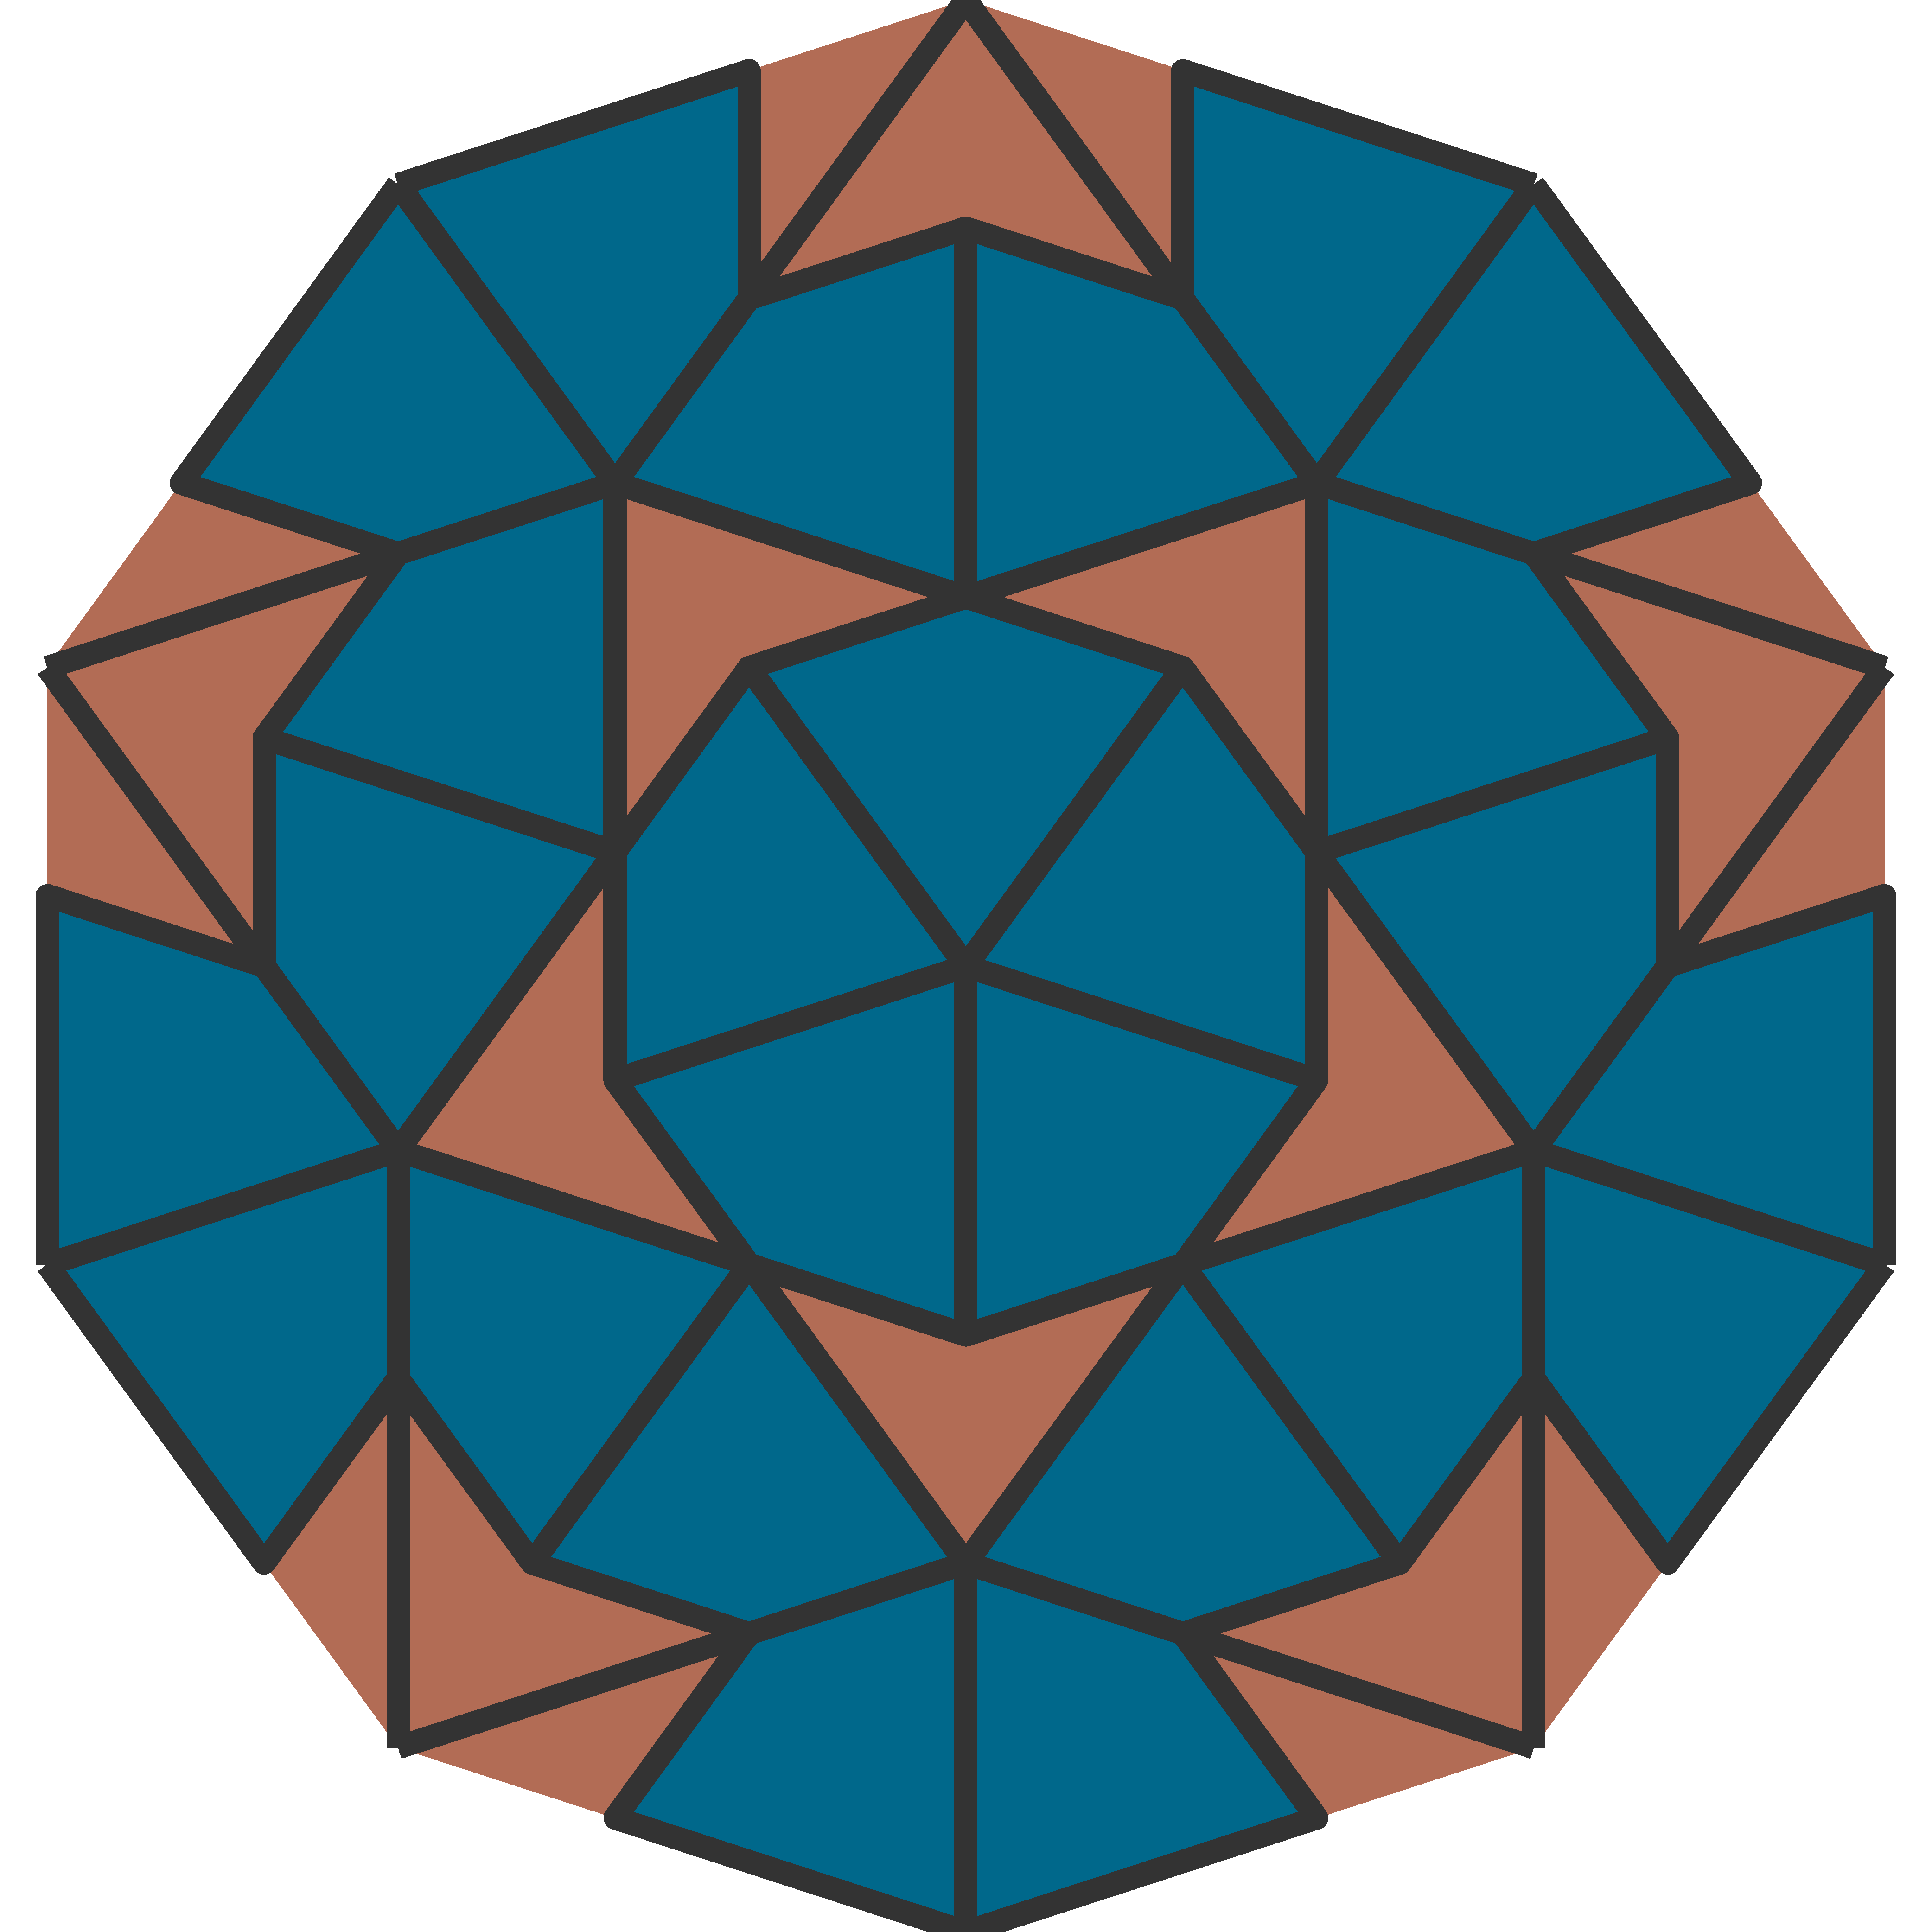
\includegraphics[width=0.9\textwidth]{img/wheel_P2_2.pdf}
\>
\)
}
\only<3>{
\(
\<{6cm}
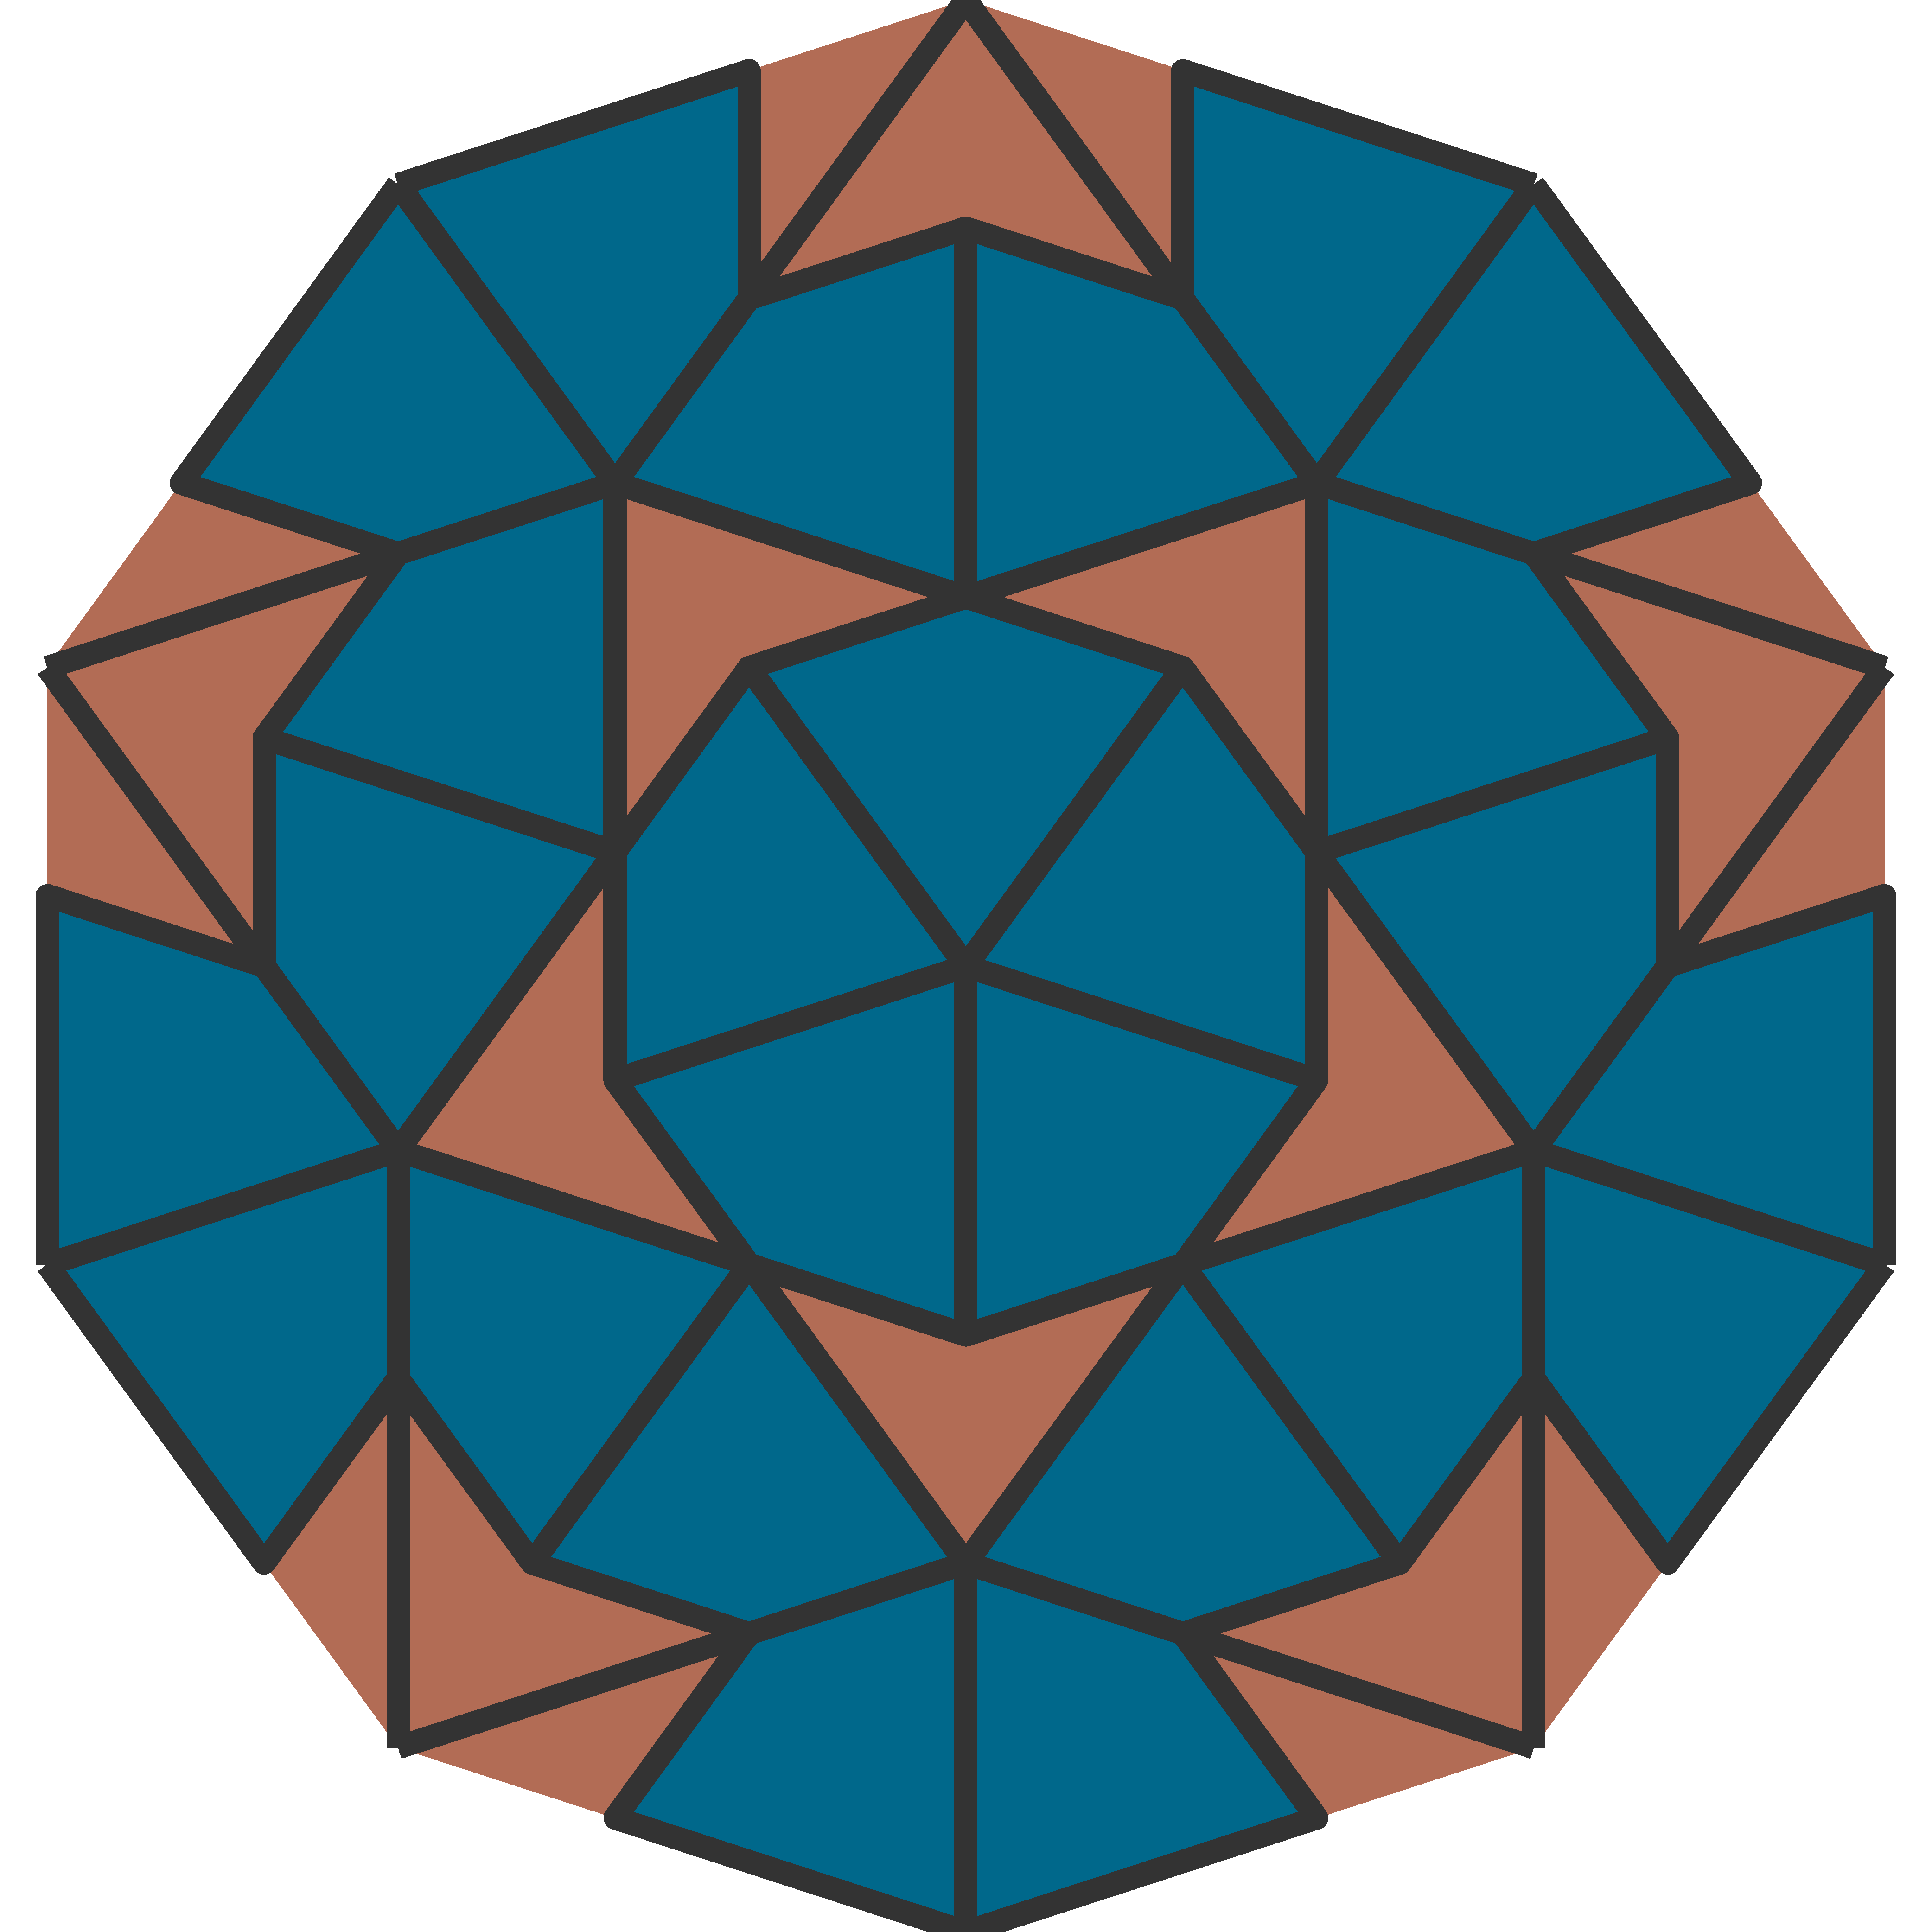
\includegraphics[width=0.9\textwidth]{img/wheel_P2_2.pdf}
\>
\<{6cm}
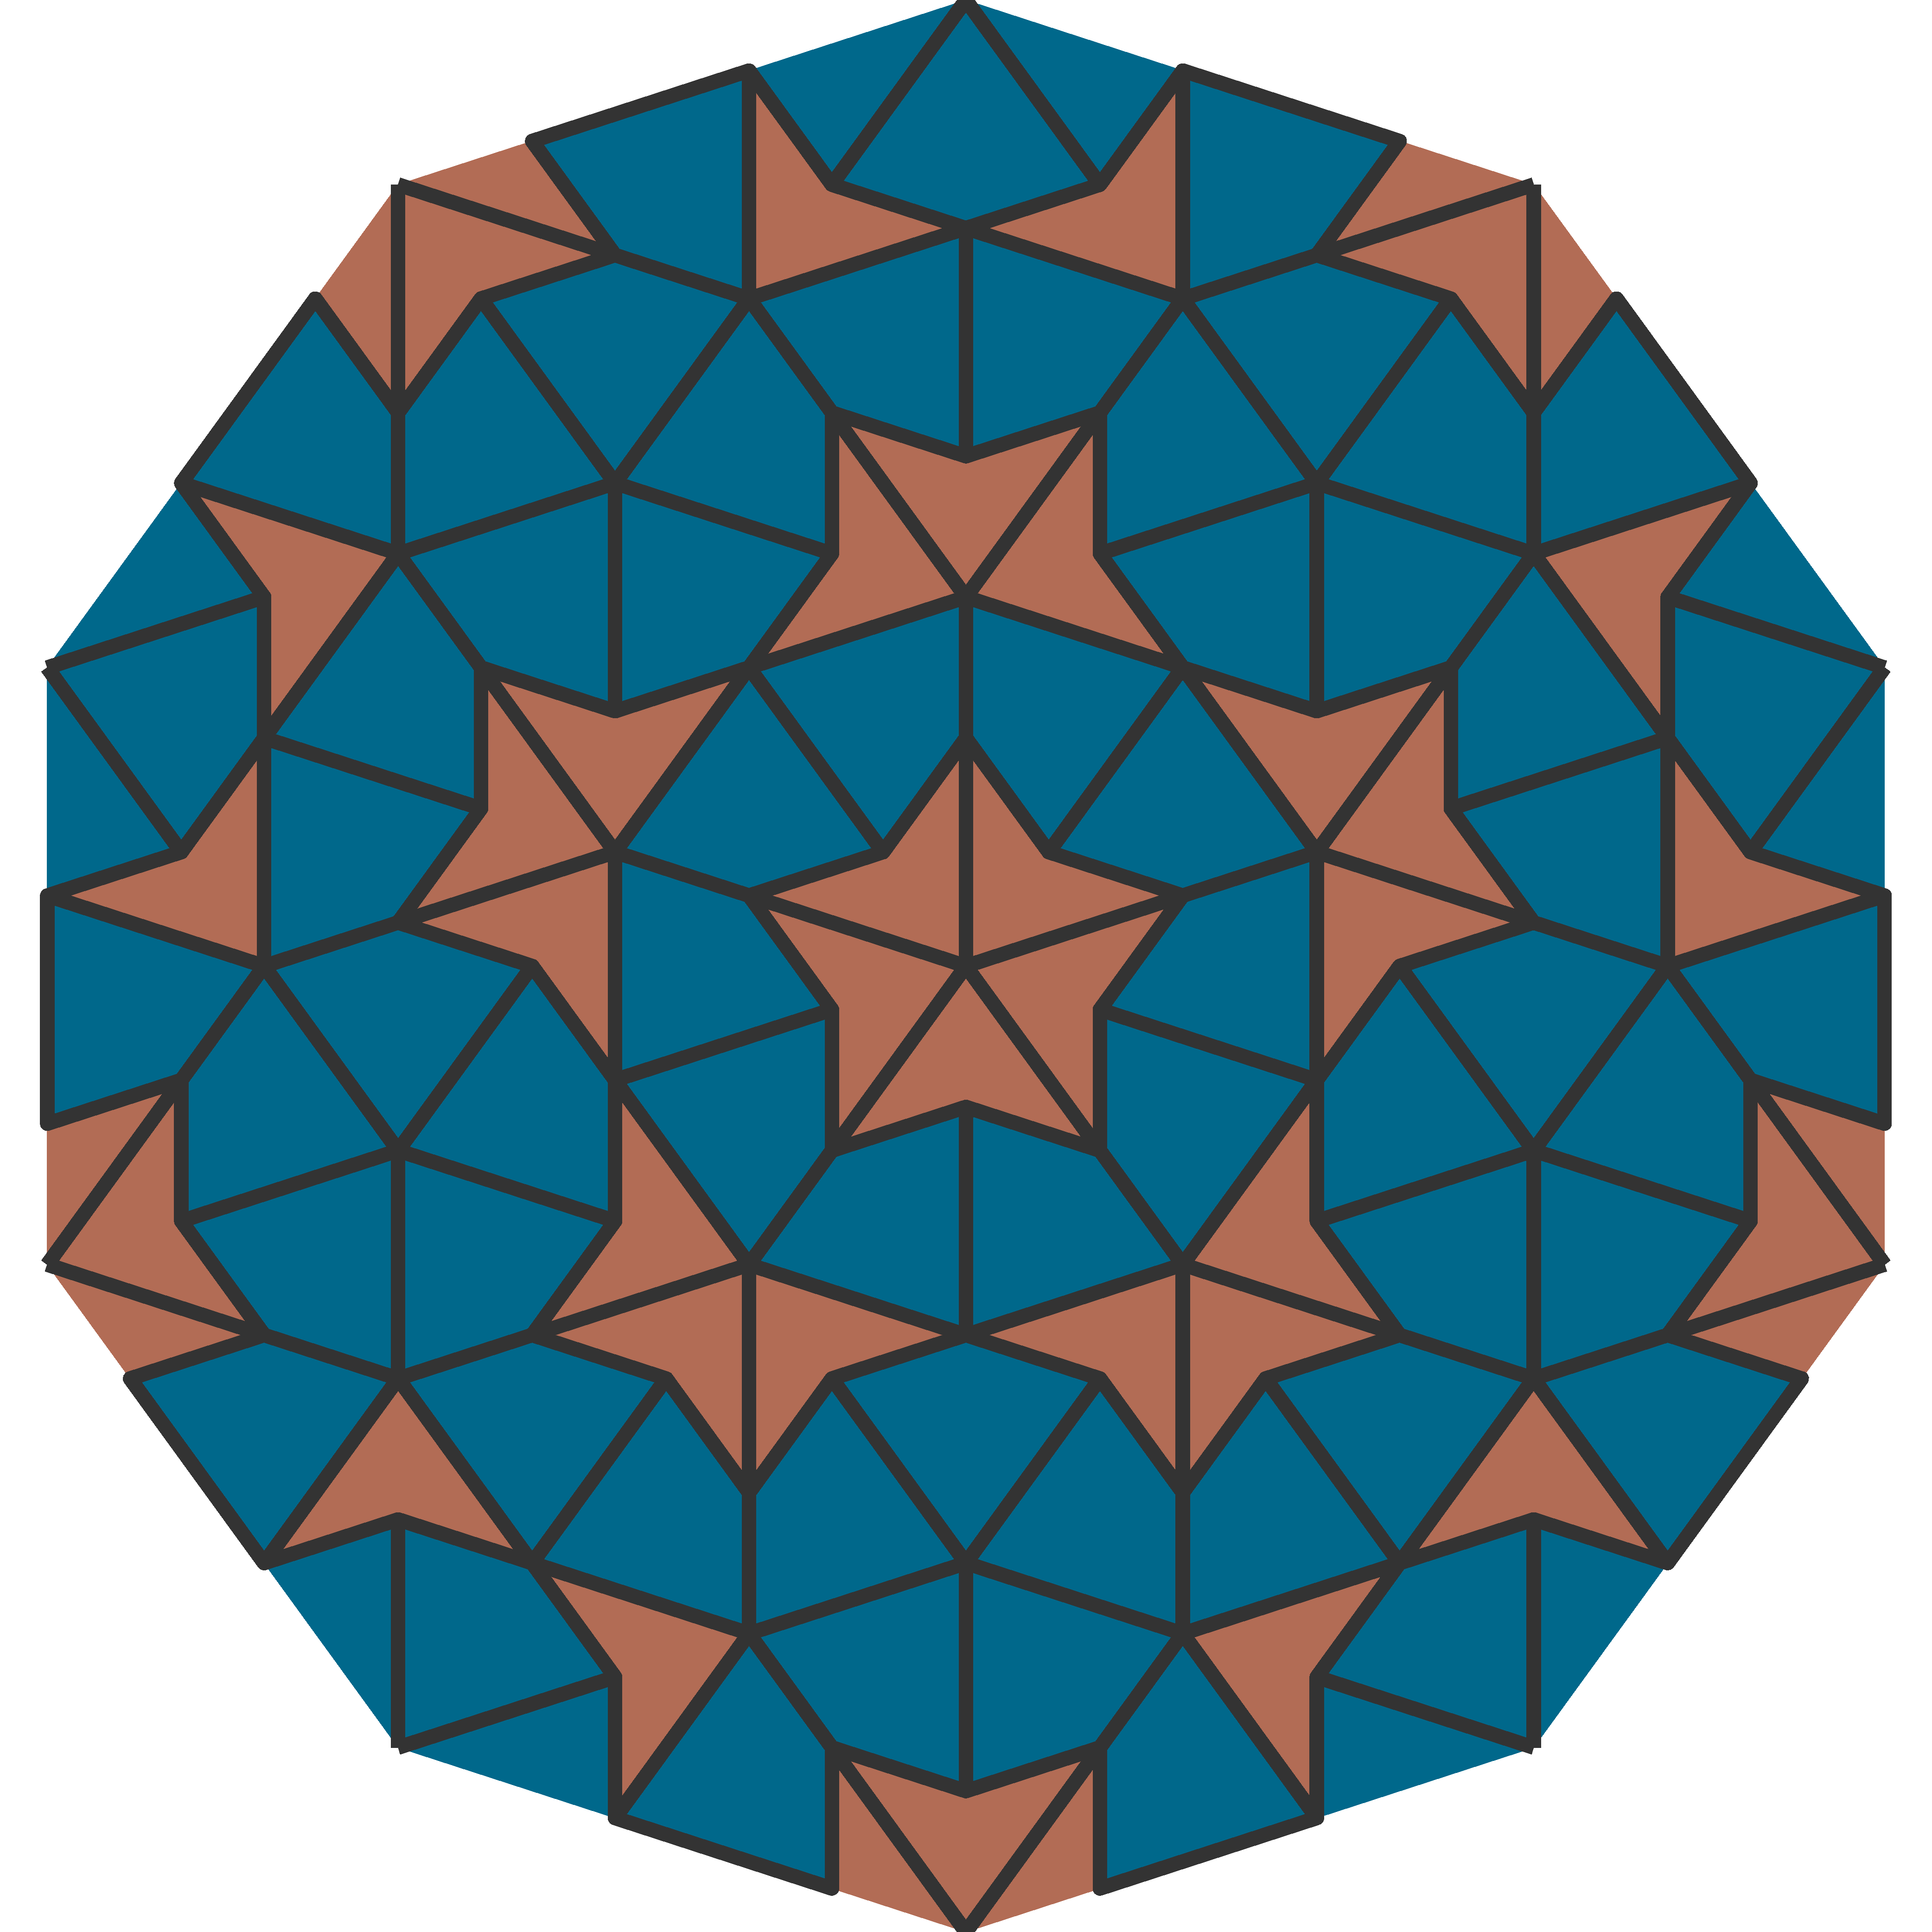
\includegraphics[width=0.9\textwidth]{img/wheel_P2_3.pdf}
\>
\)
}
\only<4>{
\(
\<{6cm}
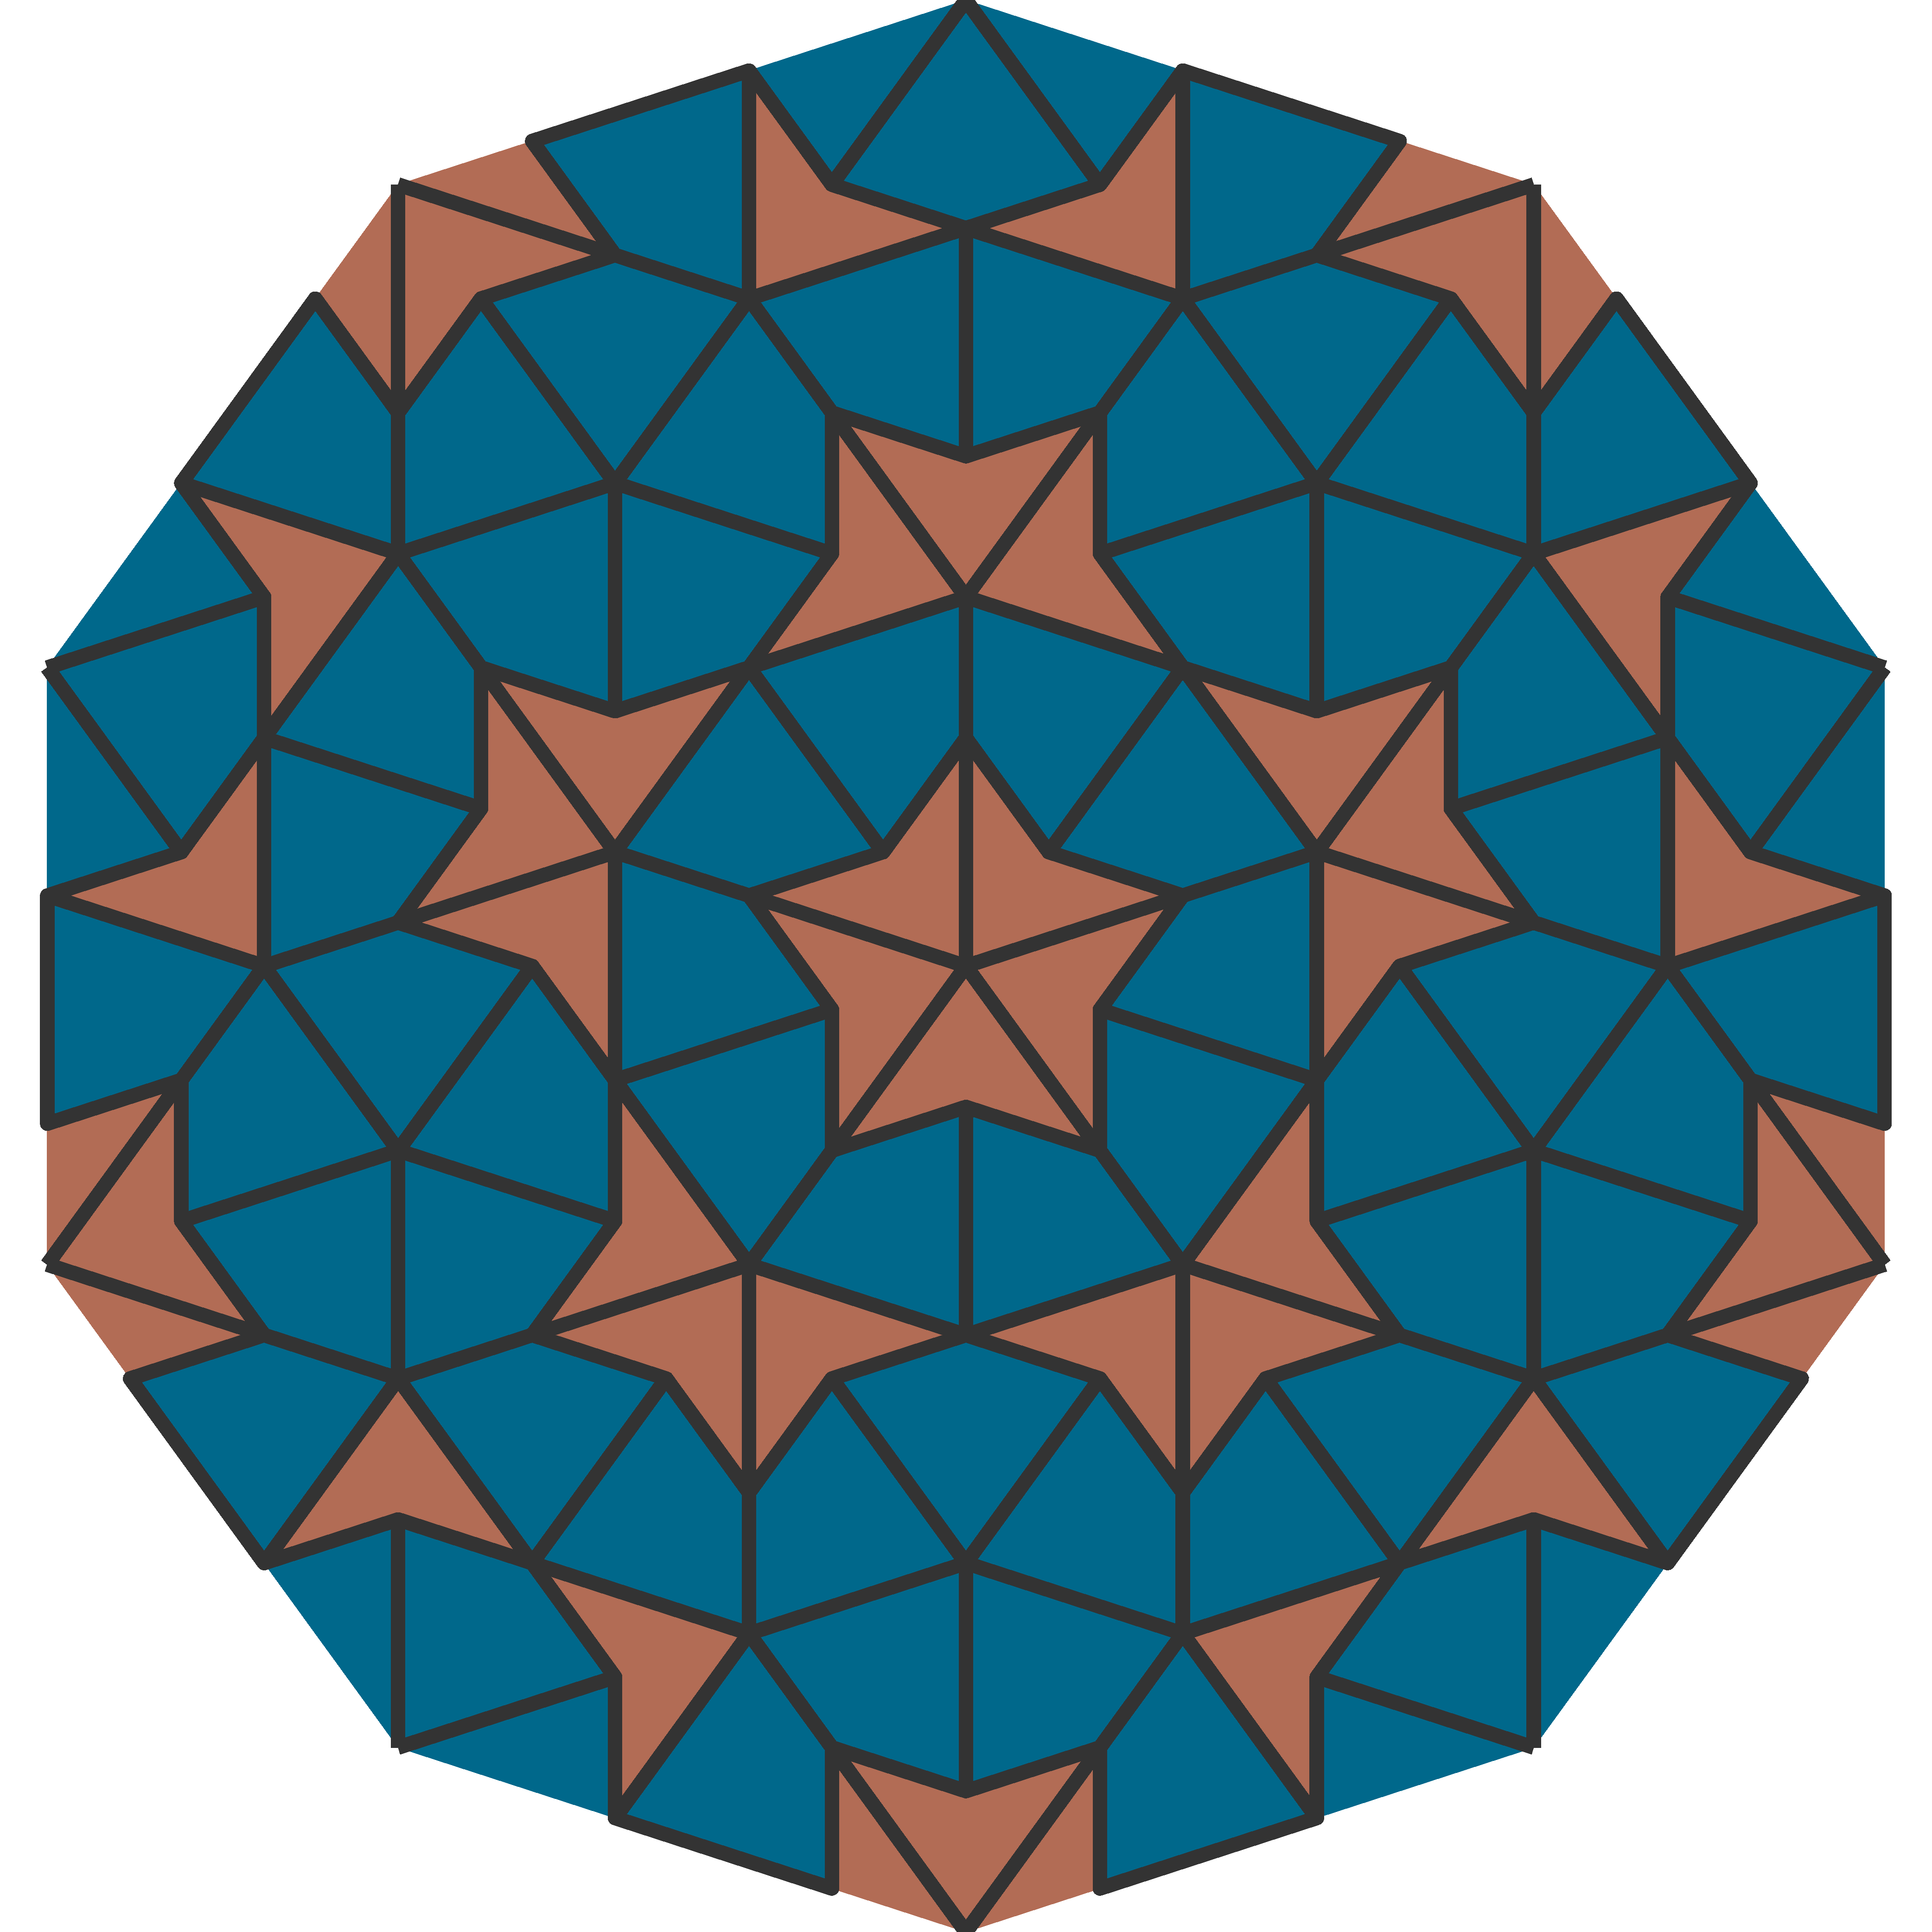
\includegraphics[width=0.9\textwidth]{img/wheel_P2_3.pdf}
\>
\<{6cm}
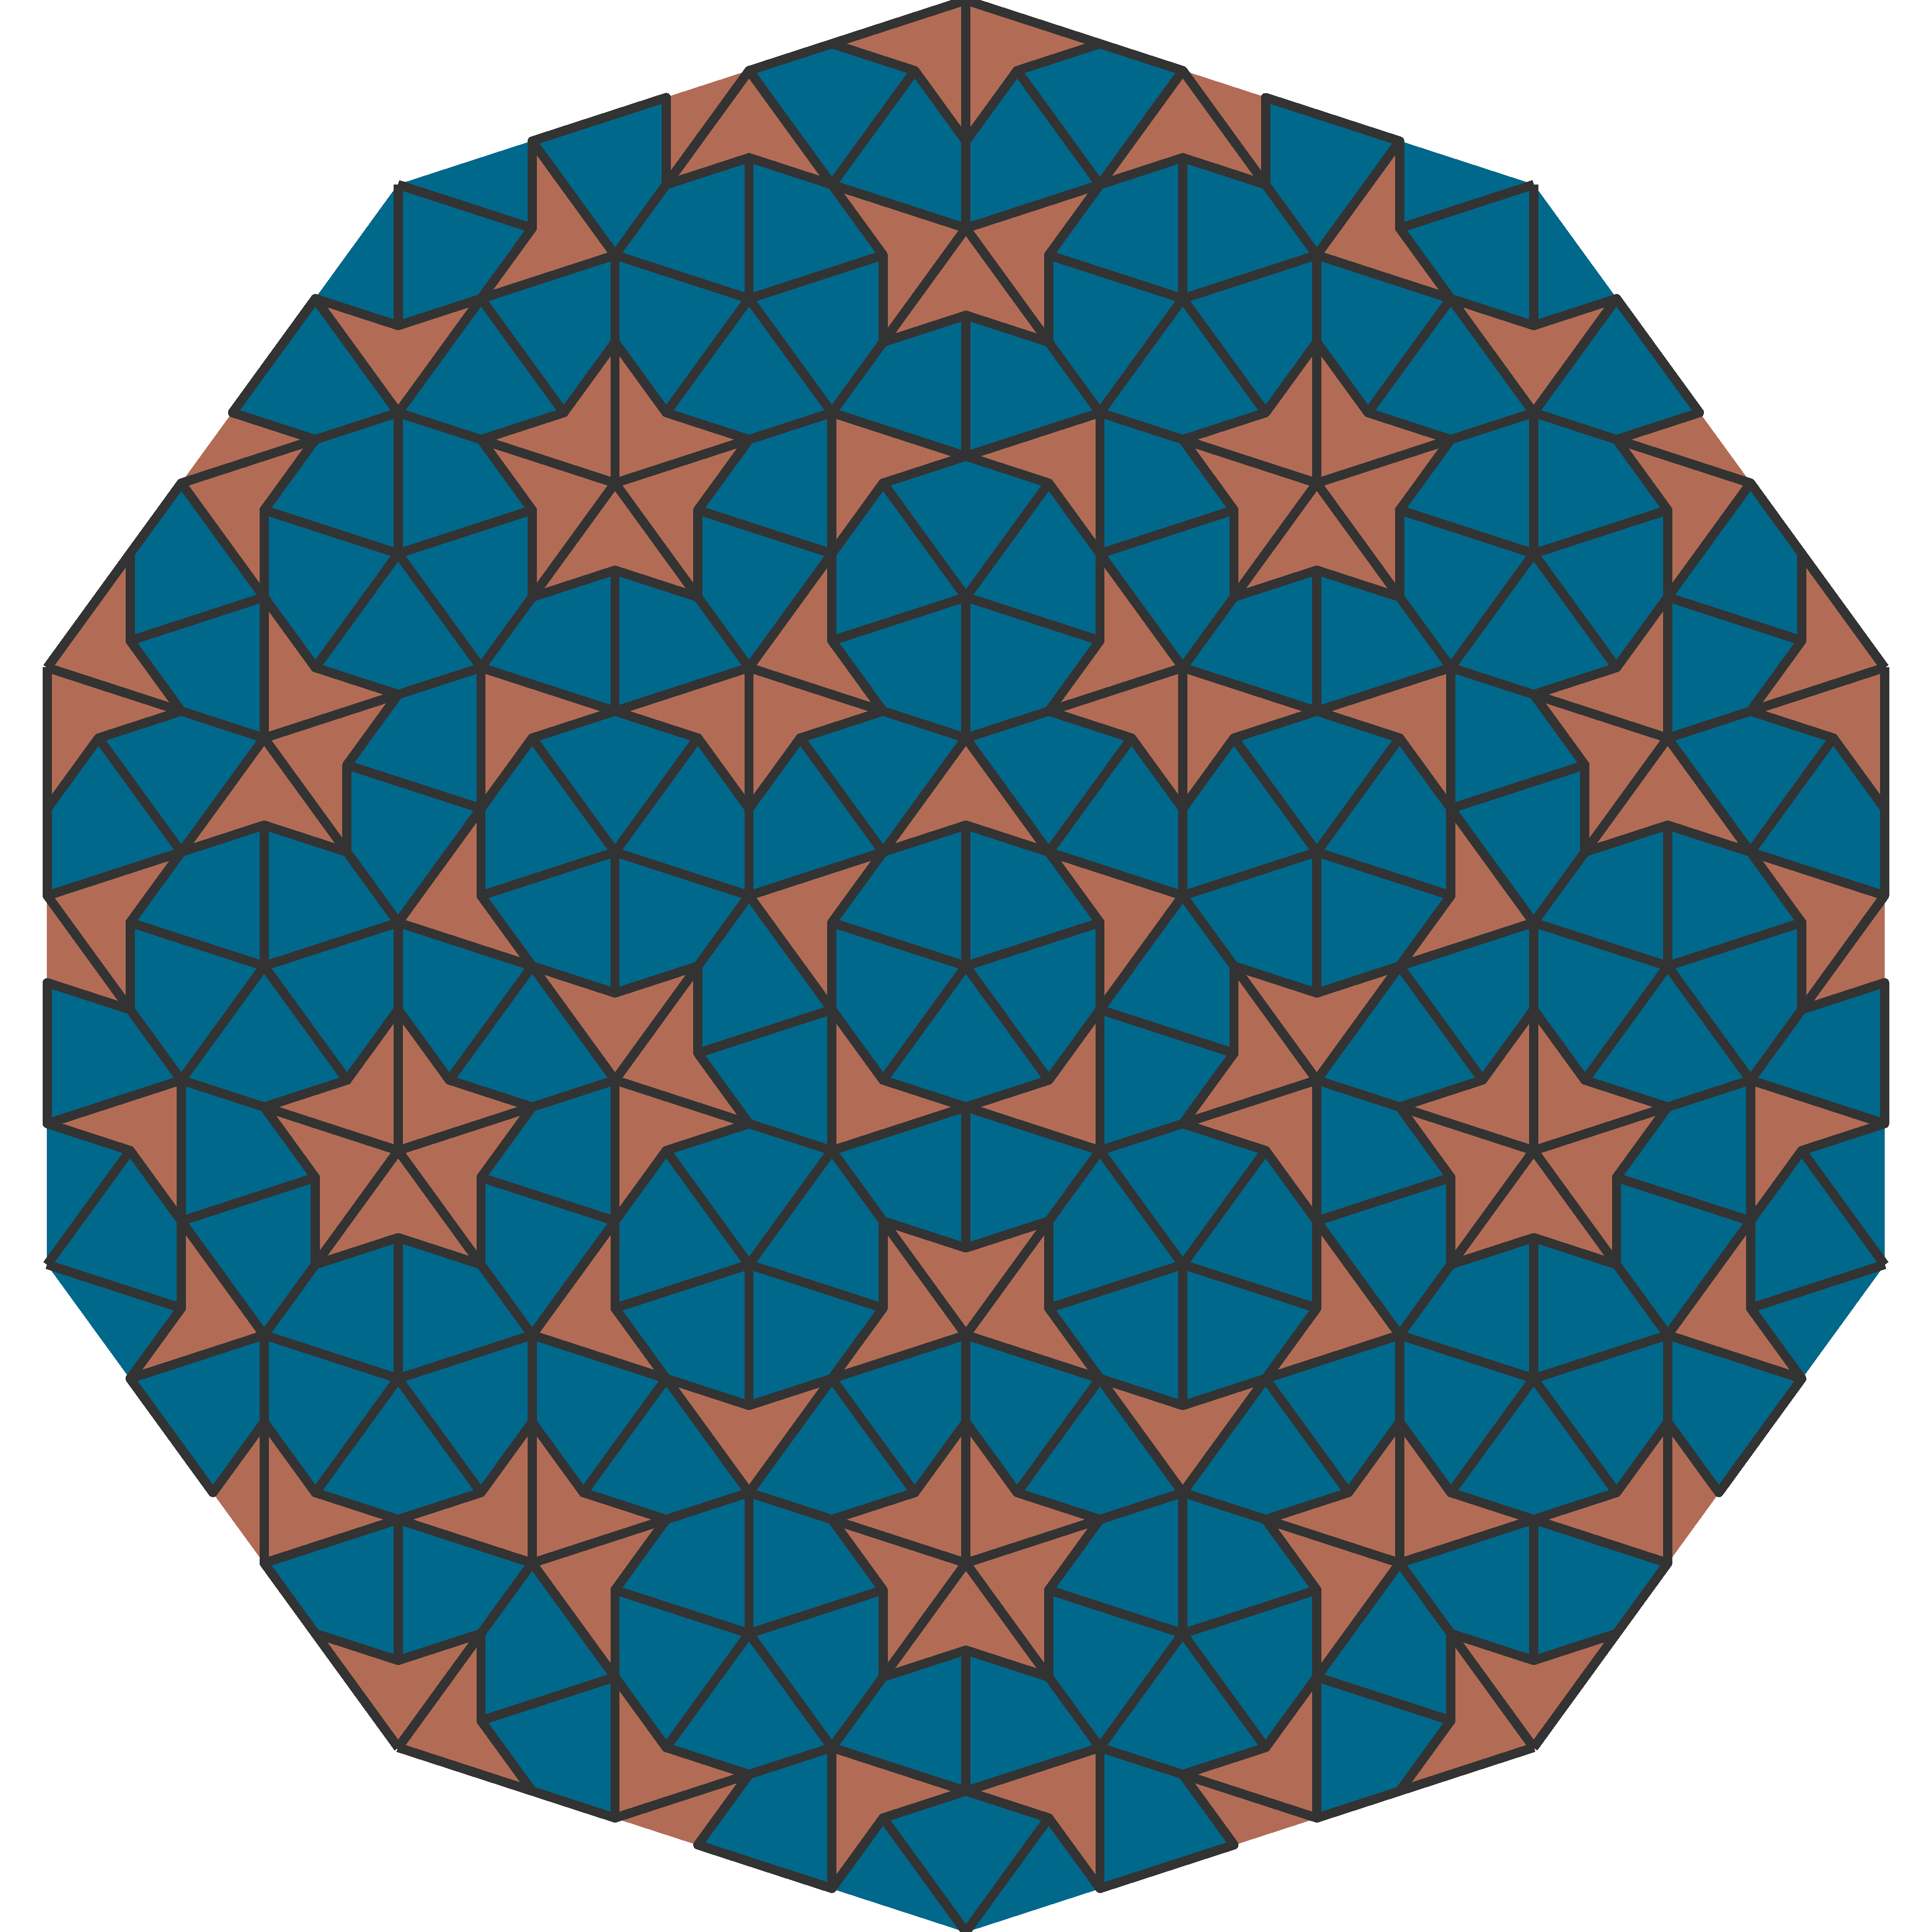
\includegraphics[width=0.9\textwidth]{img/wheel_P2_4.pdf}
\>
\)
}
\only<5>{
\(
\<{6cm}
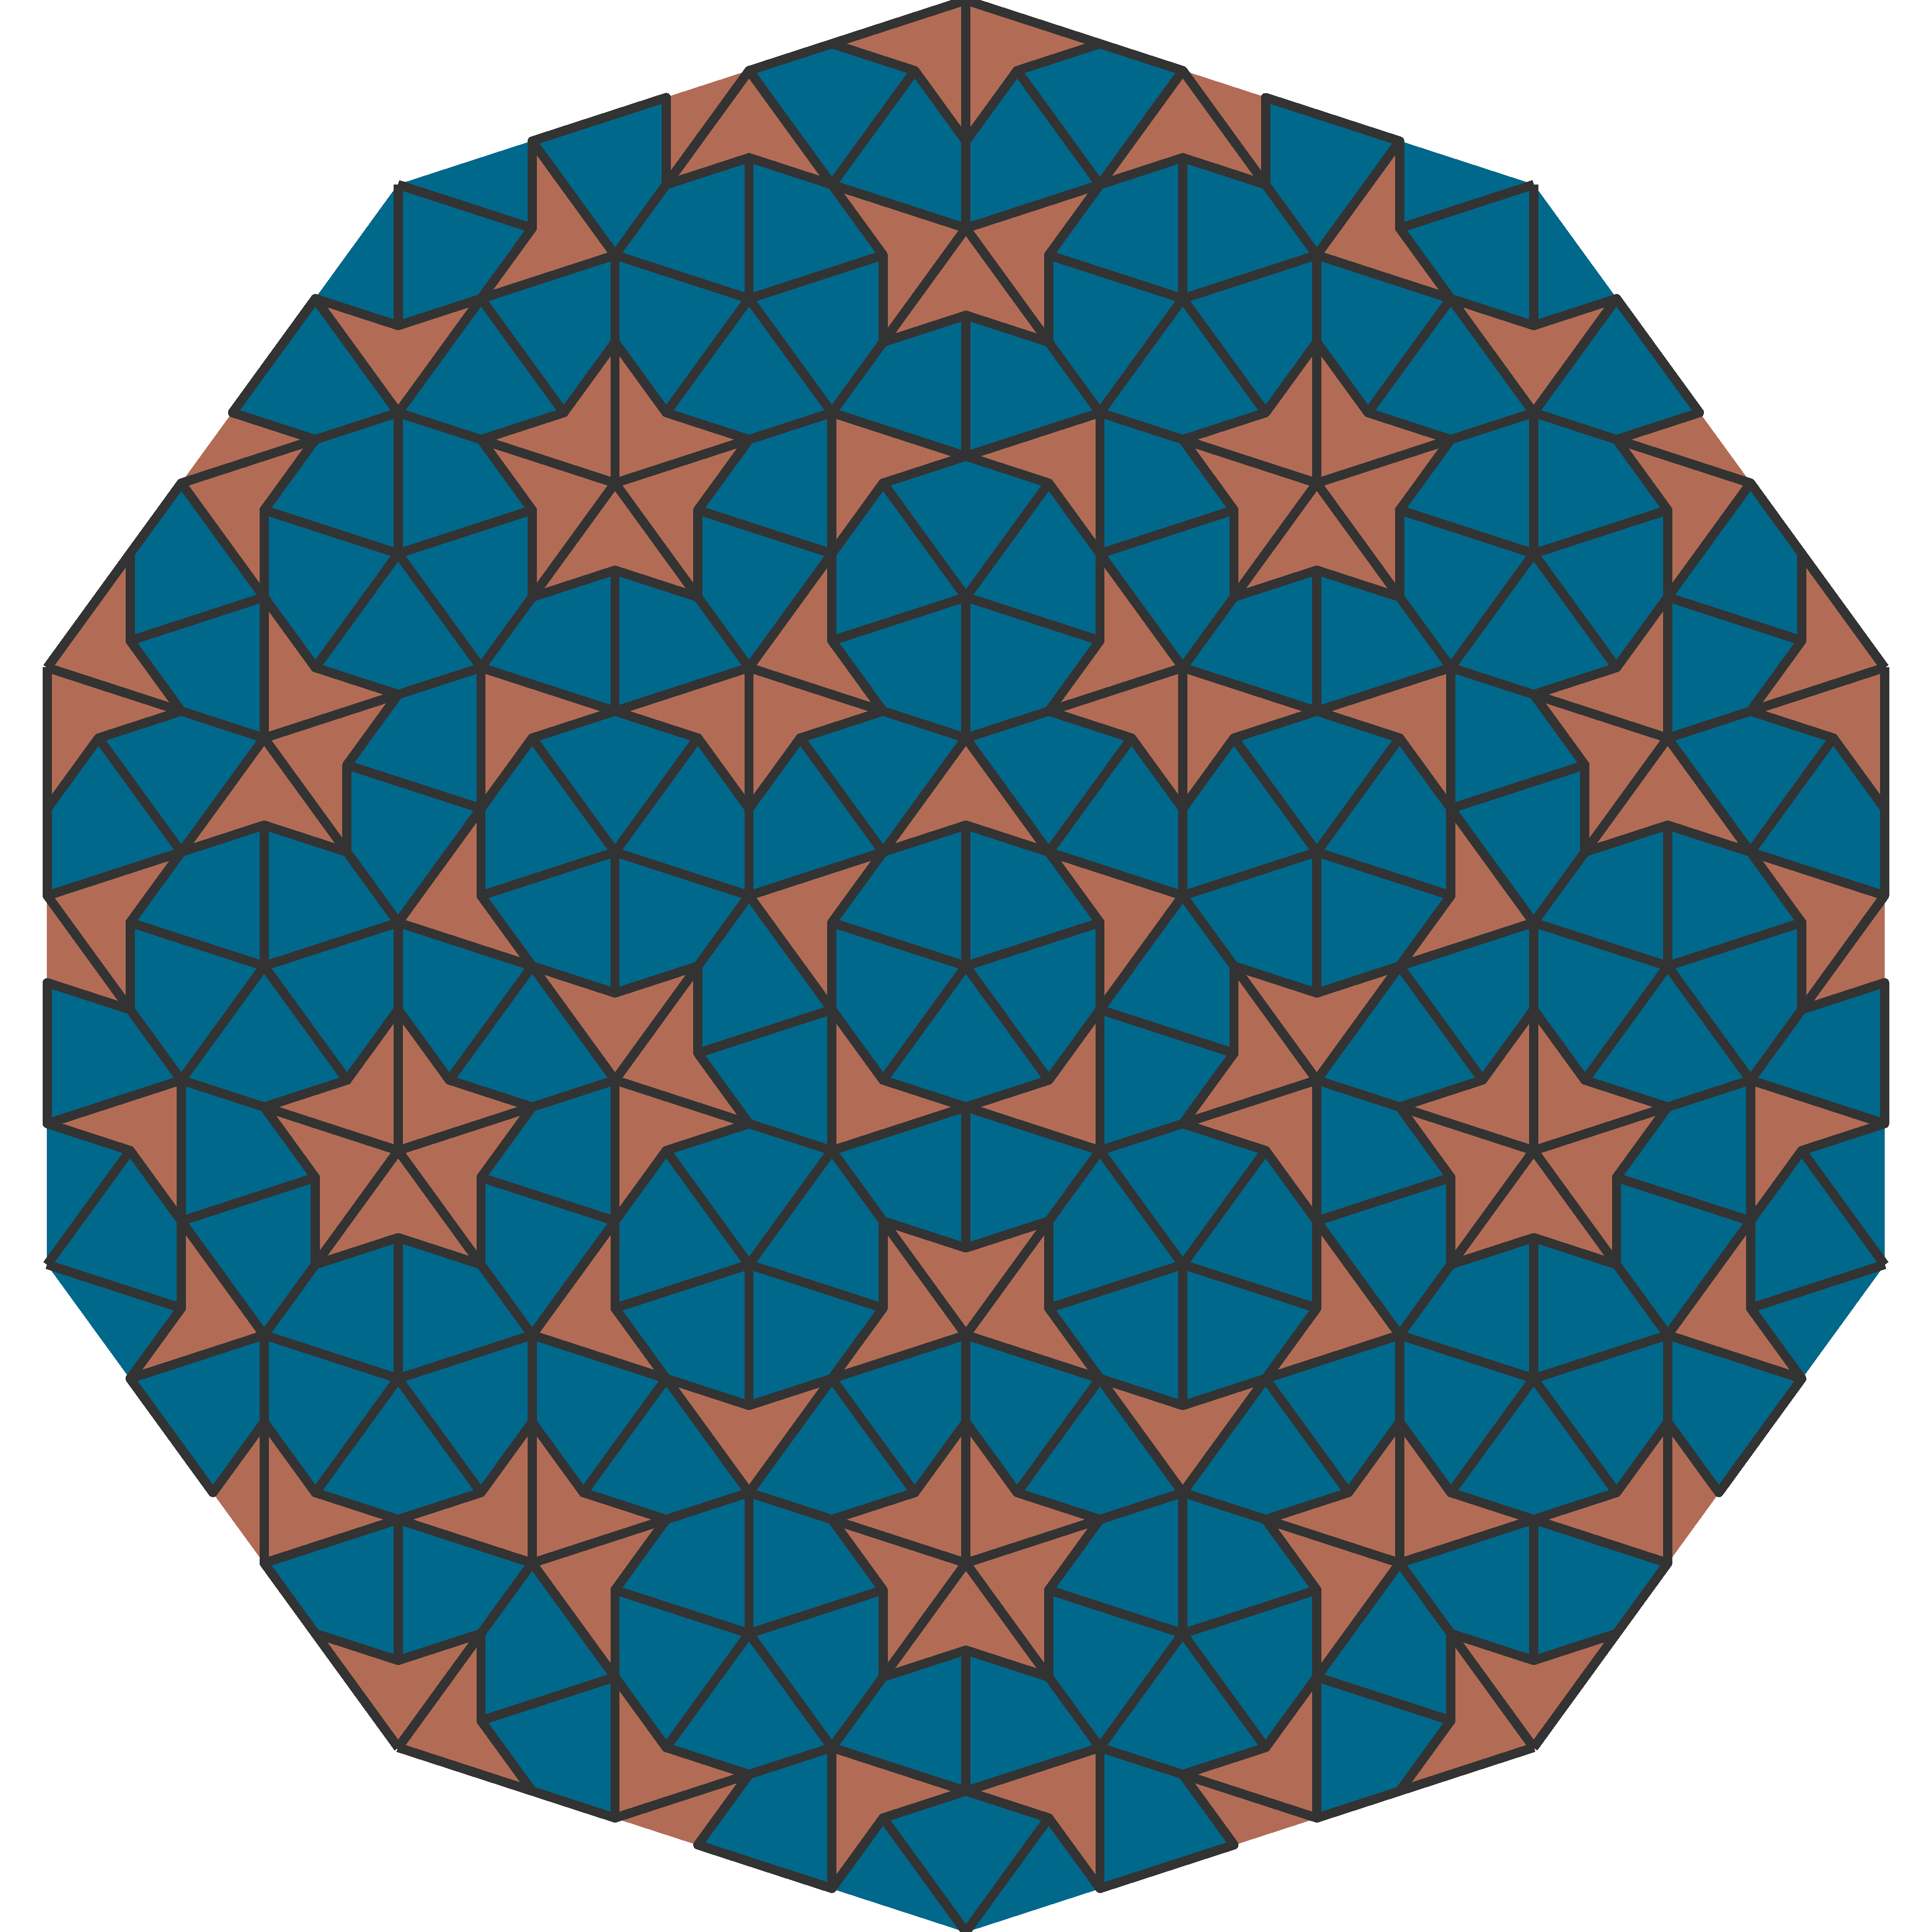
\includegraphics[width=0.9\textwidth]{img/wheel_P2_4.pdf}
\>
\<{6cm}
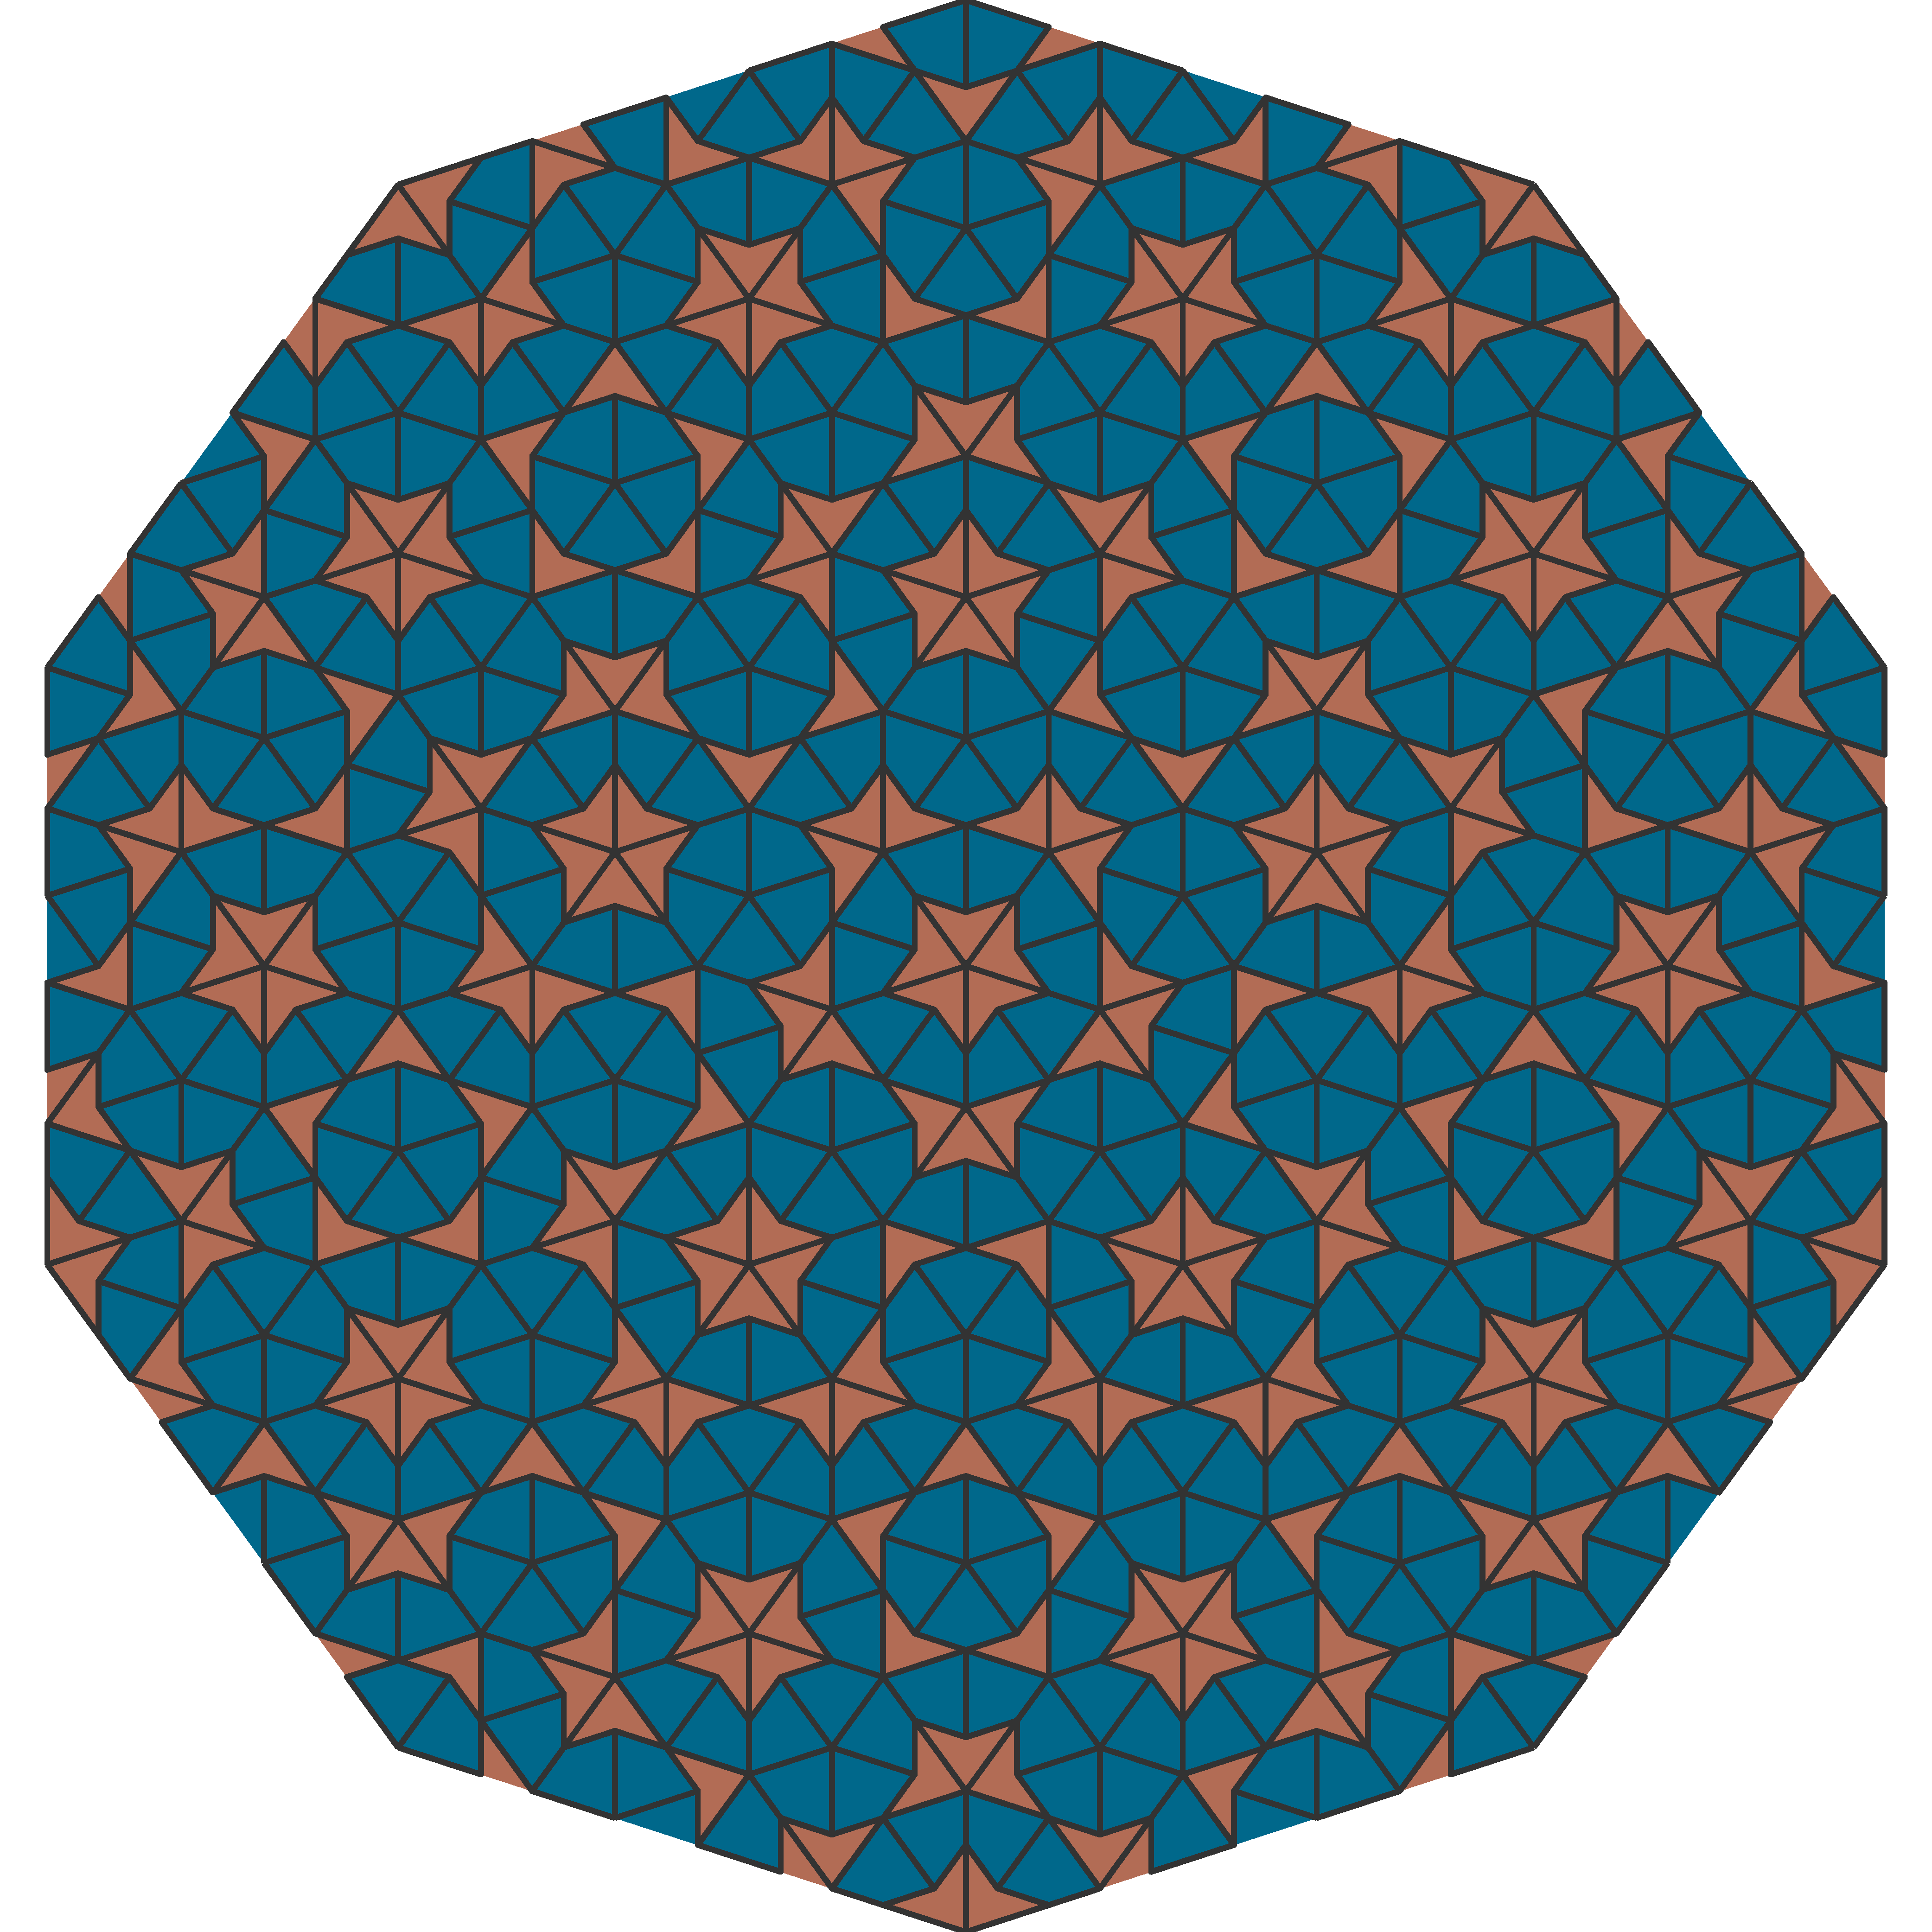
\includegraphics[width=0.9\textwidth]{img/wheel_P2_5.pdf}
\>
\)
}
\only<6>{
\(
\<{6cm}
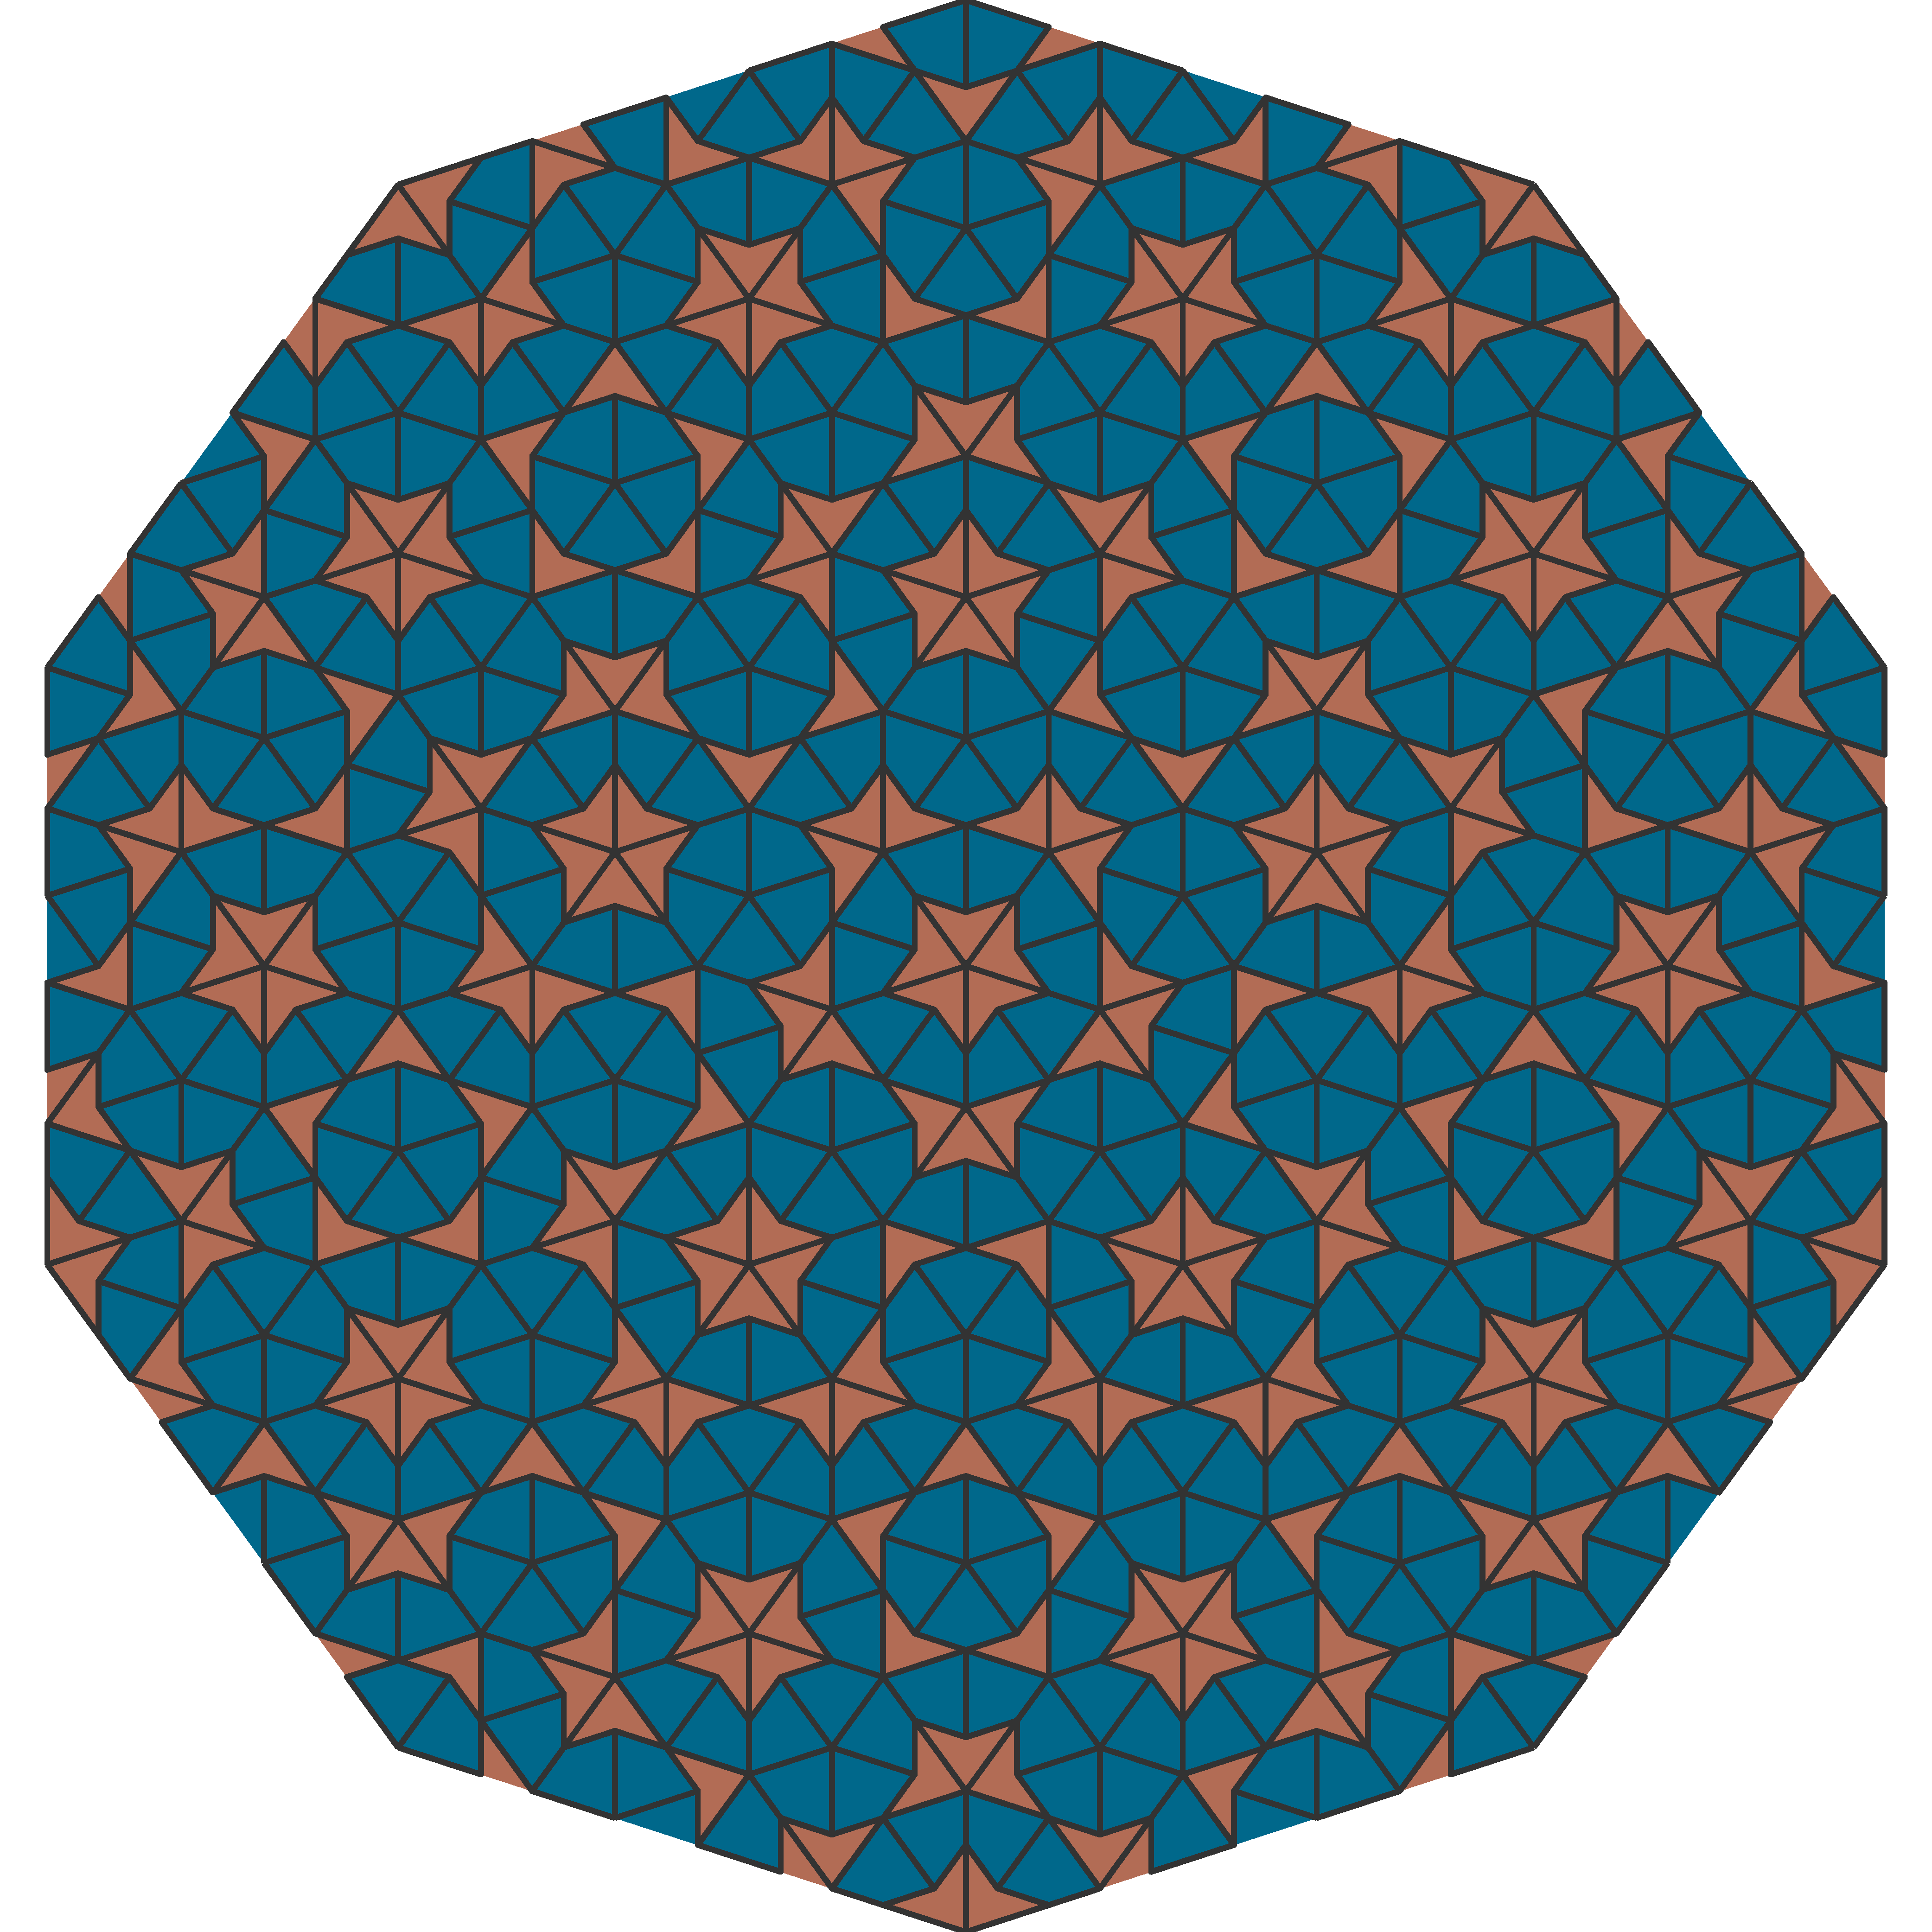
\includegraphics[width=0.9\textwidth]{img/wheel_P2_5.pdf}
\>
\<{6cm}
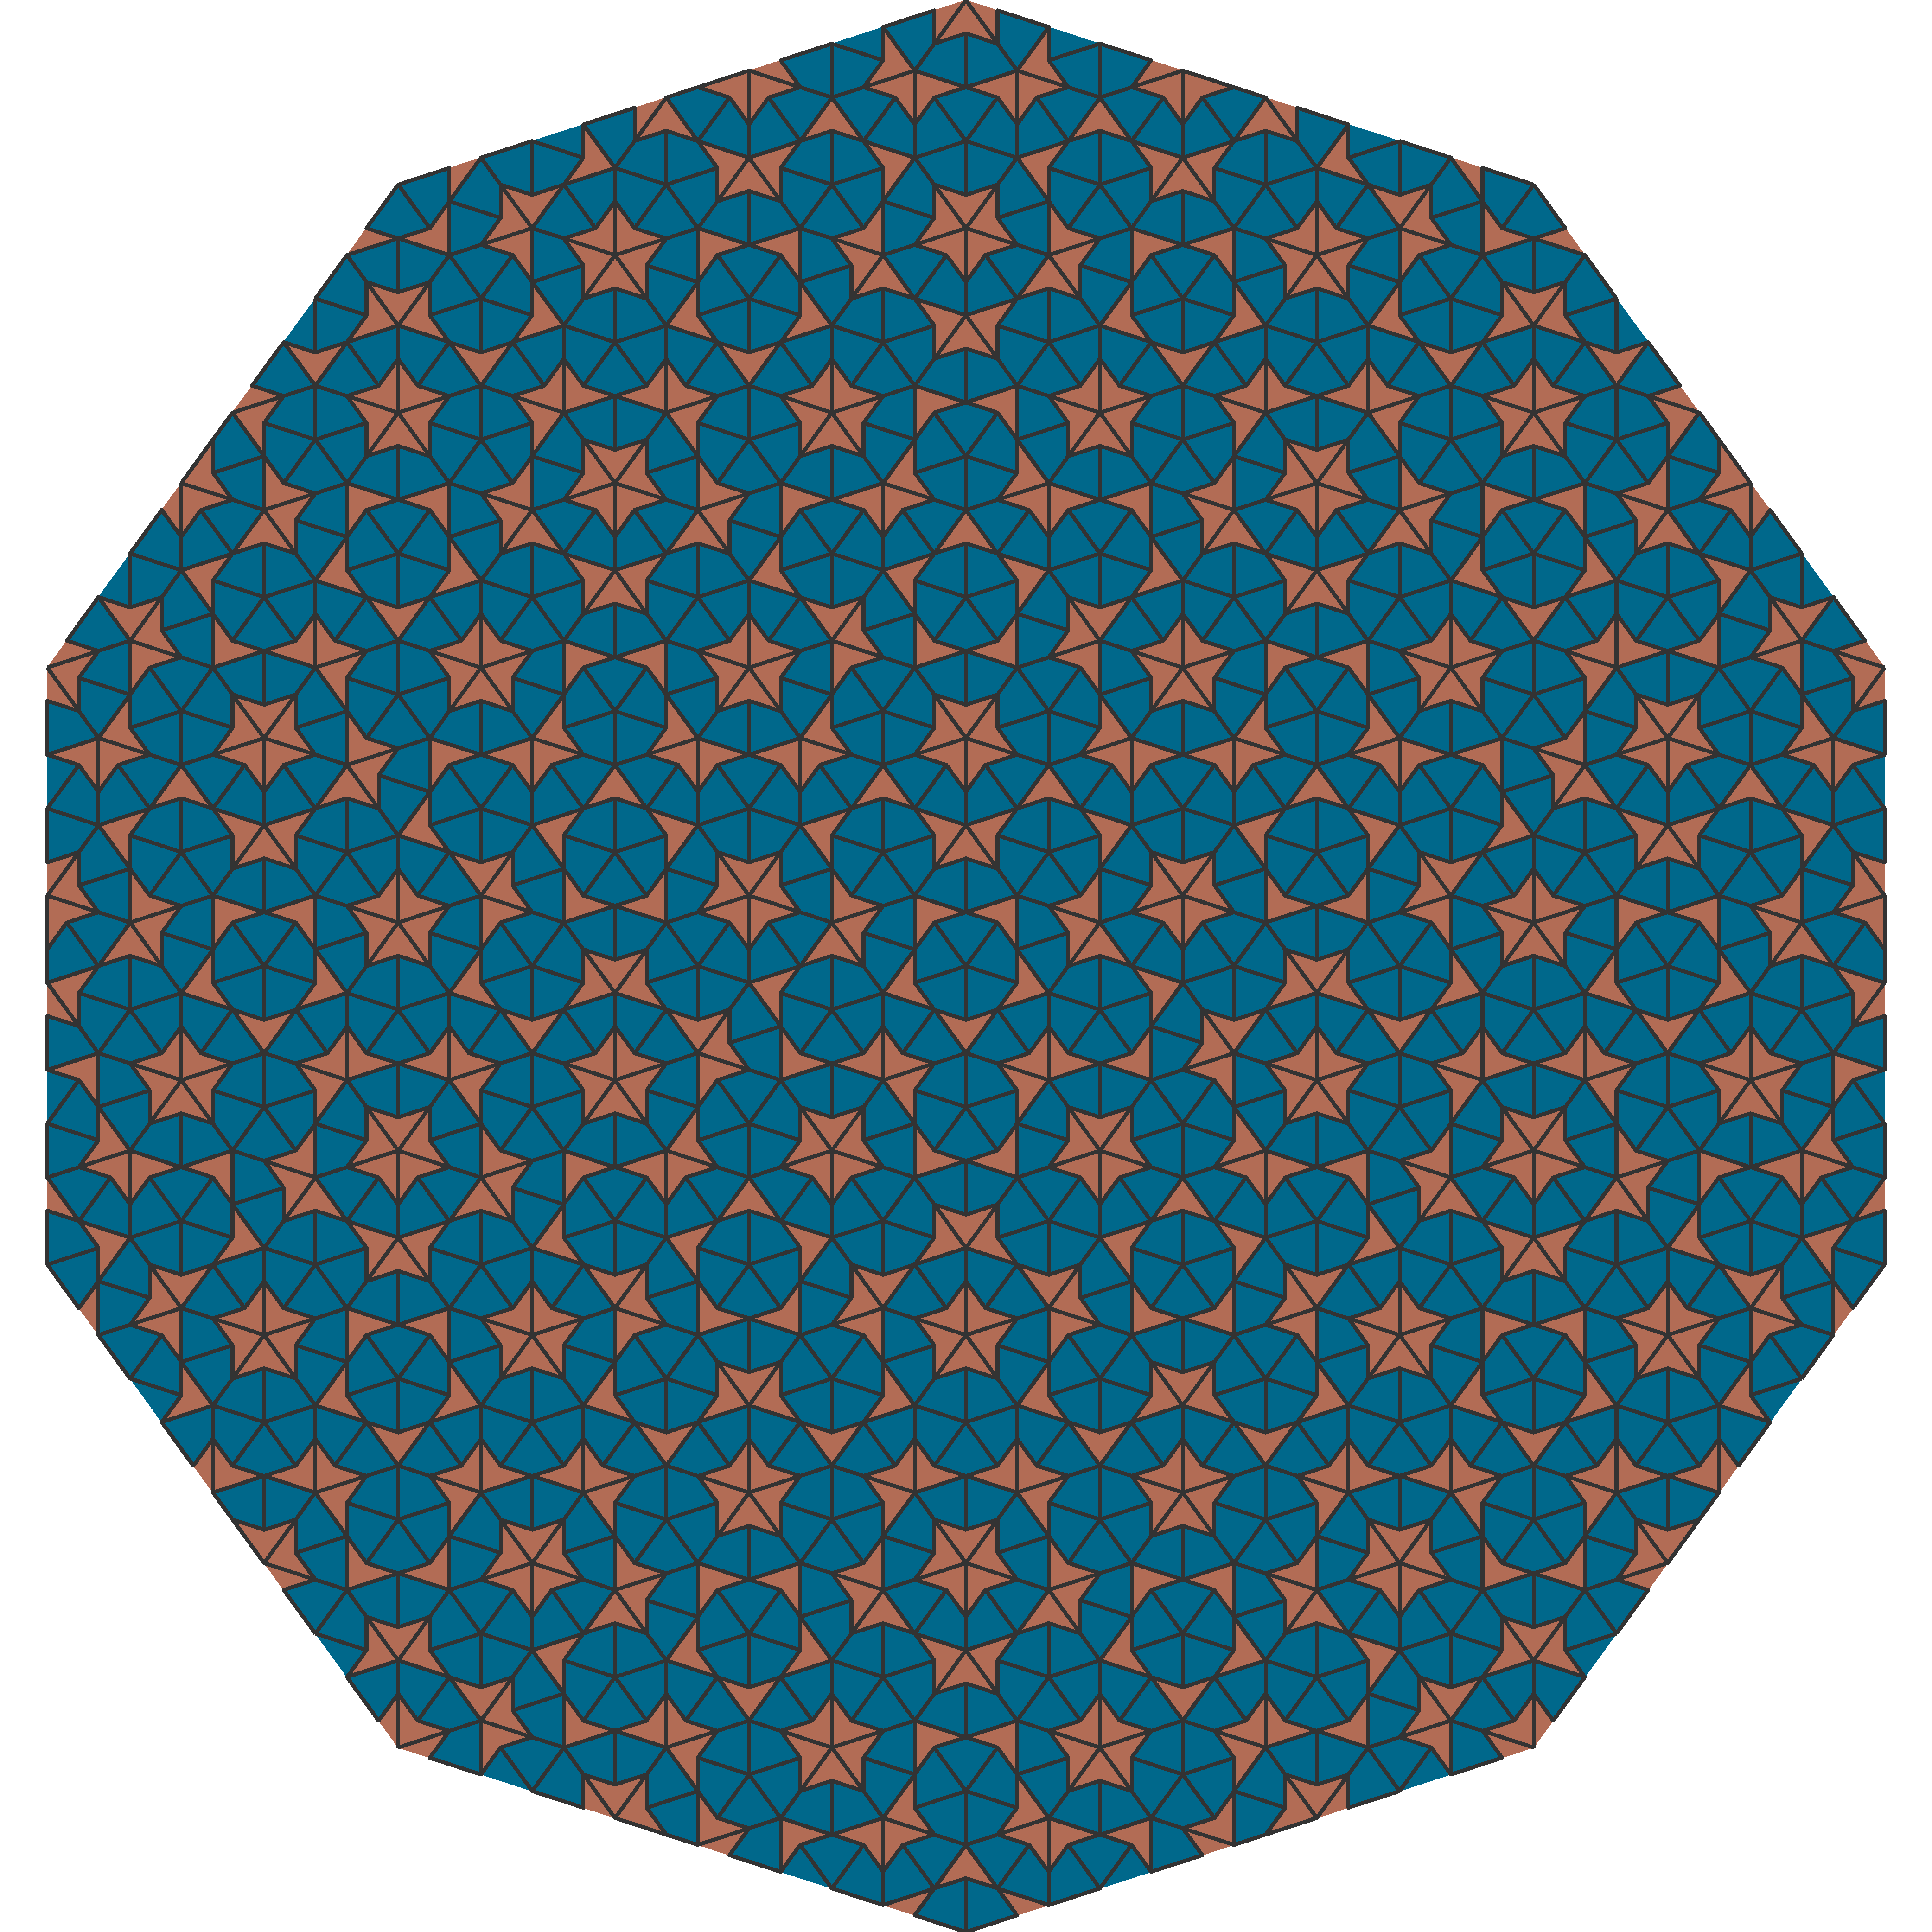
\includegraphics[width=0.9\textwidth]{img/wheel_P2_6.pdf}
\>
\)
}
\only<7>{
\(
\<{6cm}
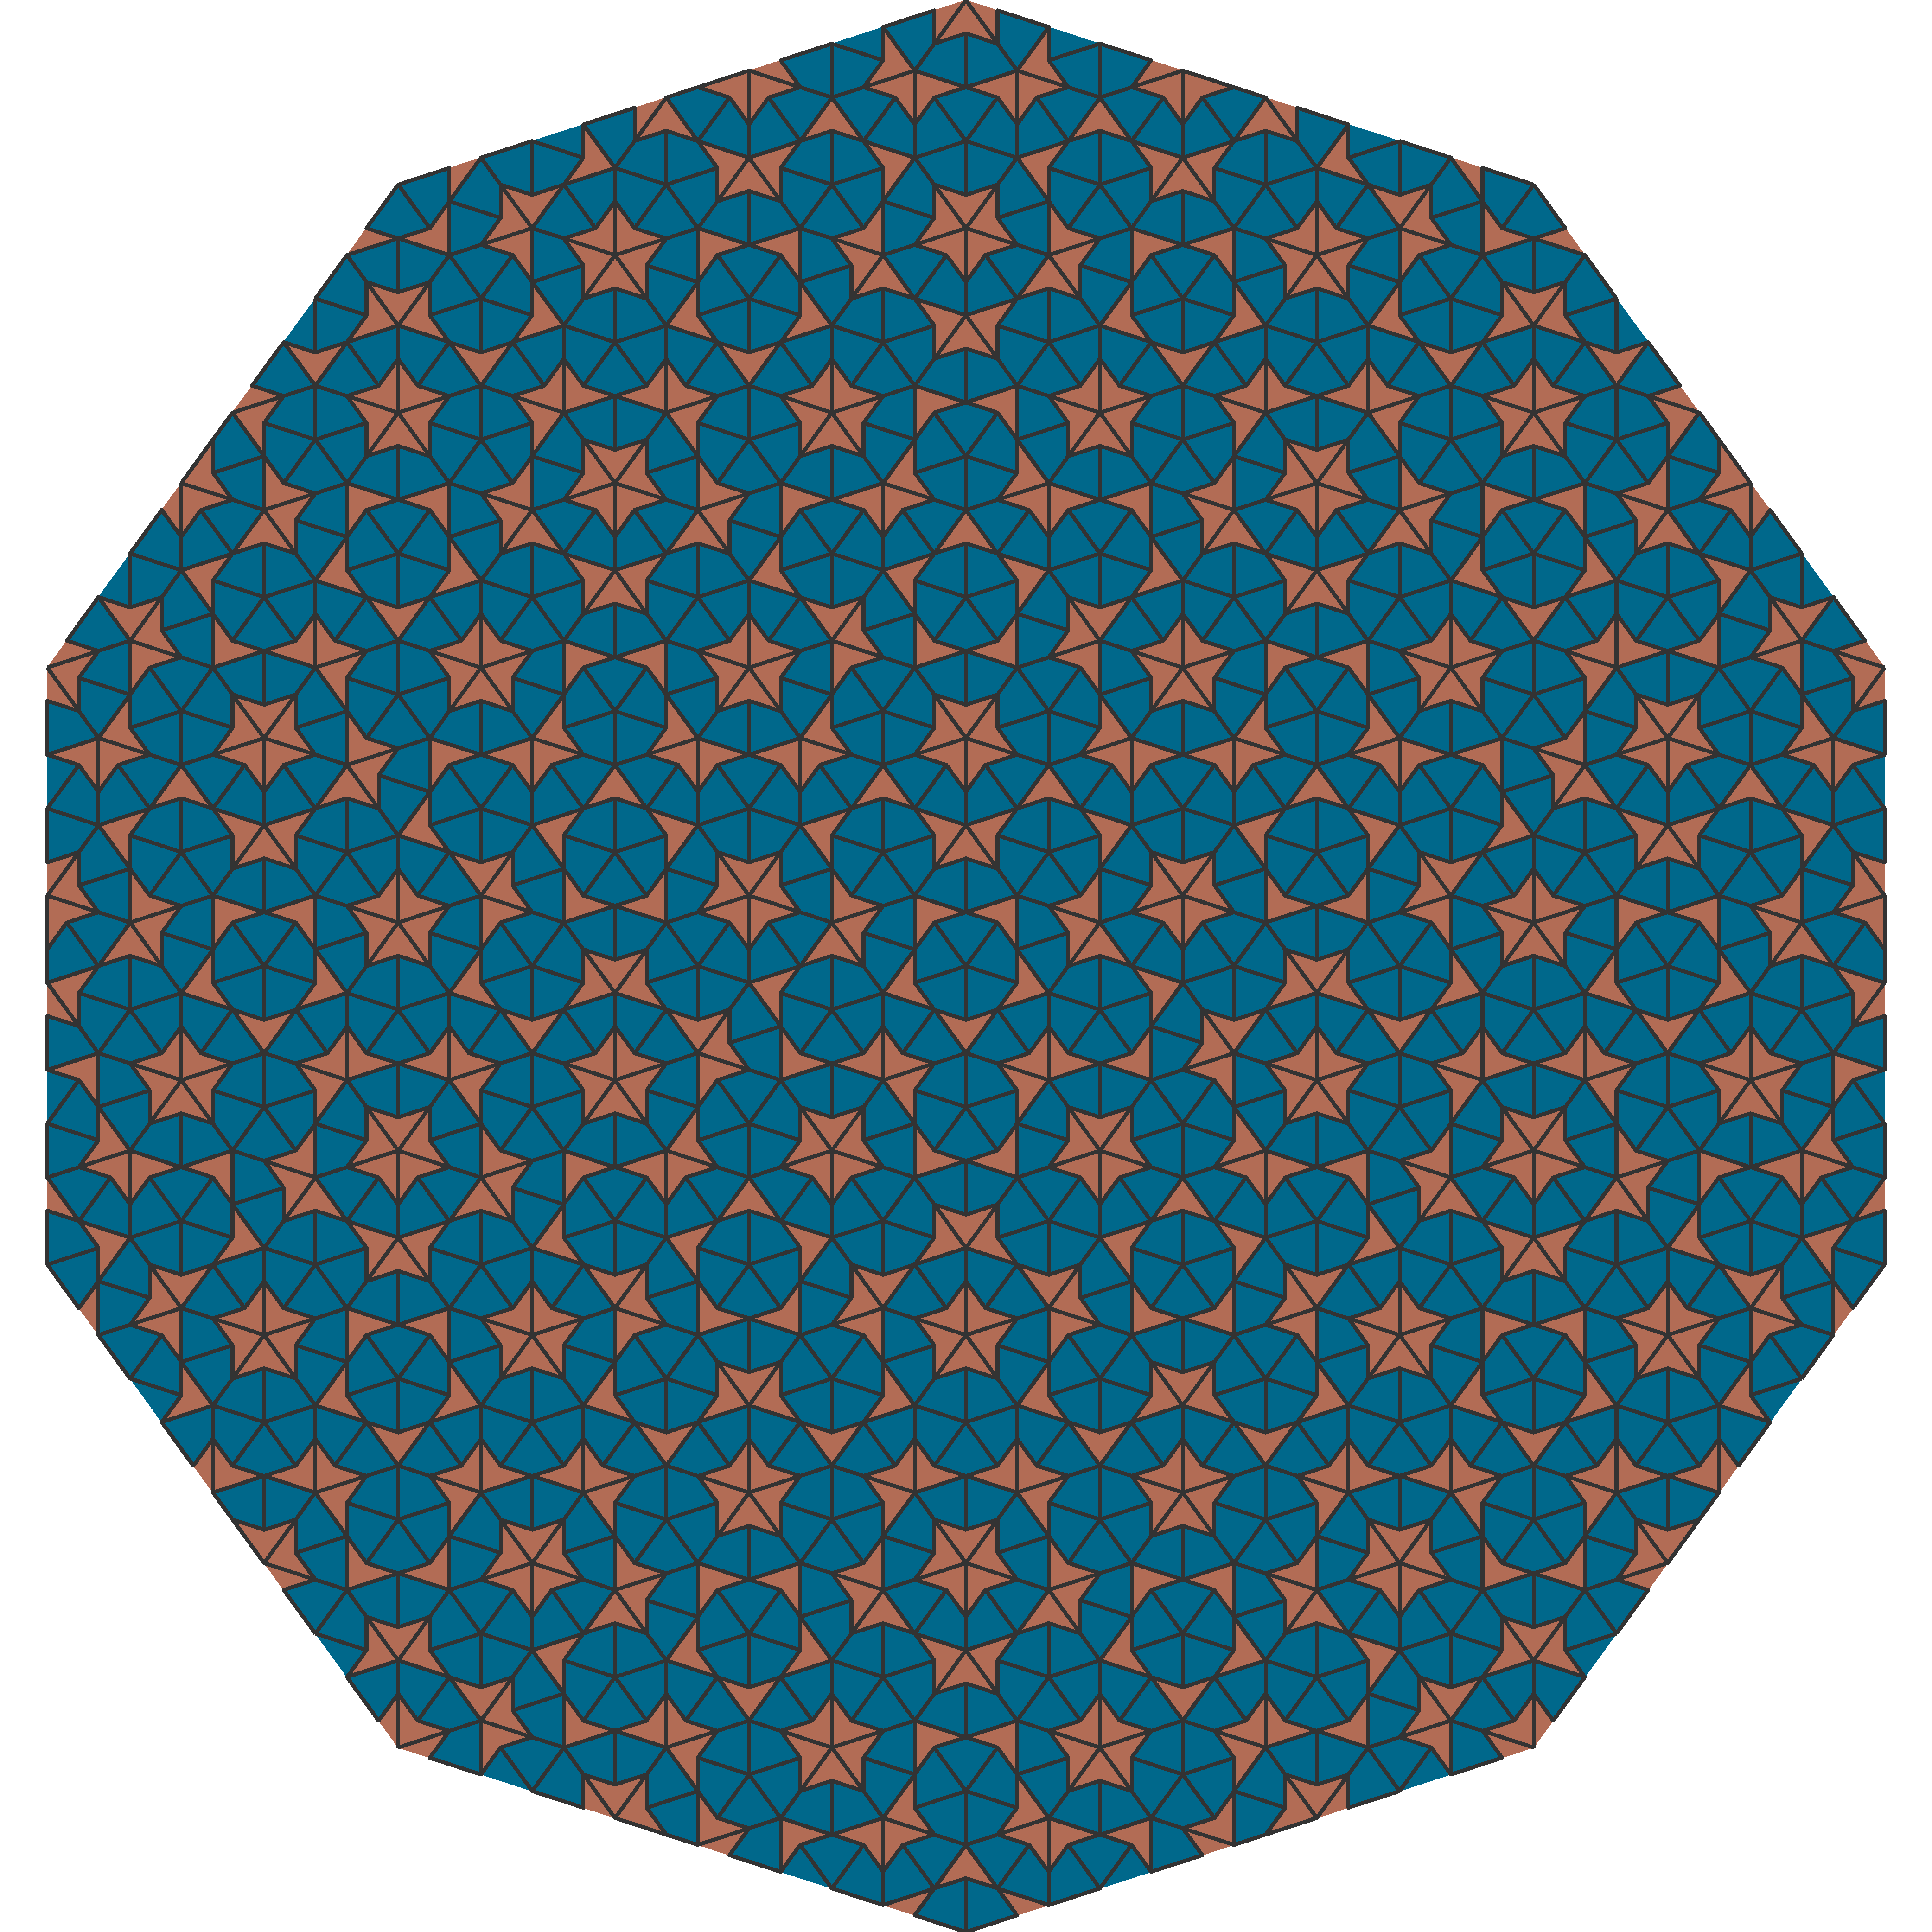
\includegraphics[width=0.9\textwidth]{img/wheel_P2_6.pdf}
\>
\<{6cm}
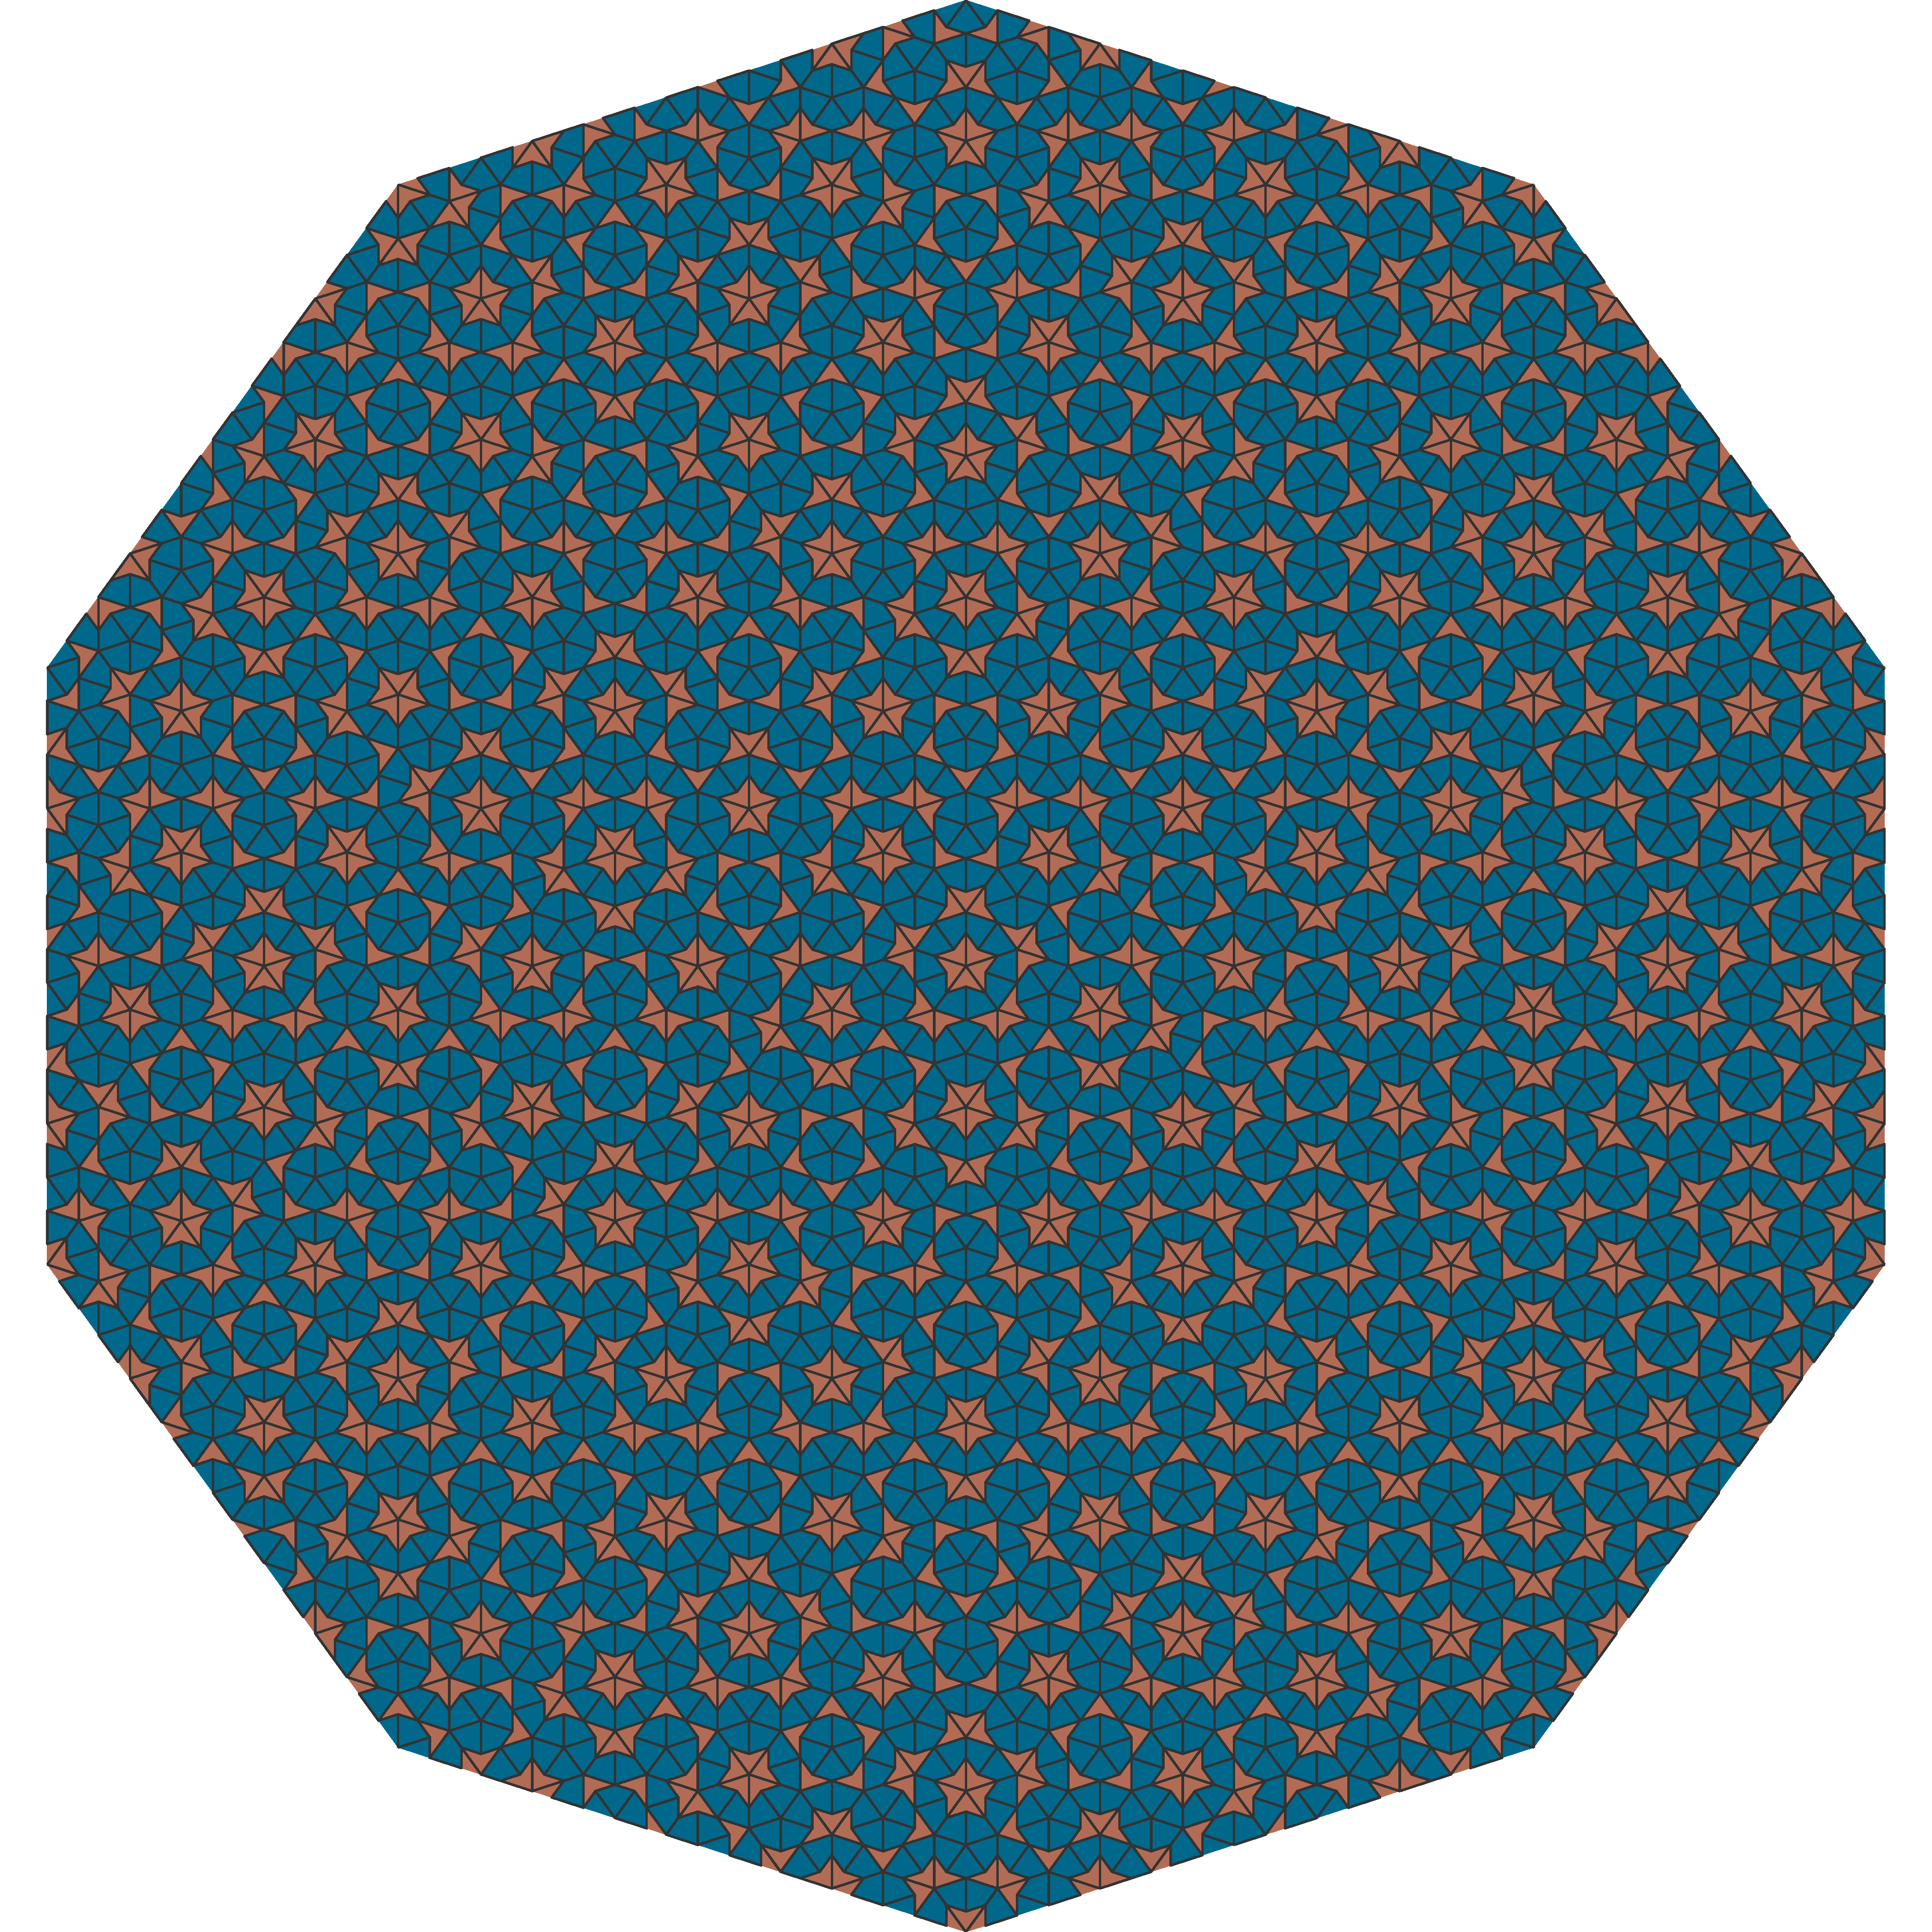
\includegraphics[width=0.9\textwidth]{img/wheel_P2_7.pdf}
\>
\)
%
\href{http://preshing.com/20110831/penrose-tiling-explained/}{preshing.com/20110831/penrose-tiling-explained}
}
\end{frame}

\begin{frame}{Presque pareil...}
\centering
\only<1>{
\(
\<{6cm}
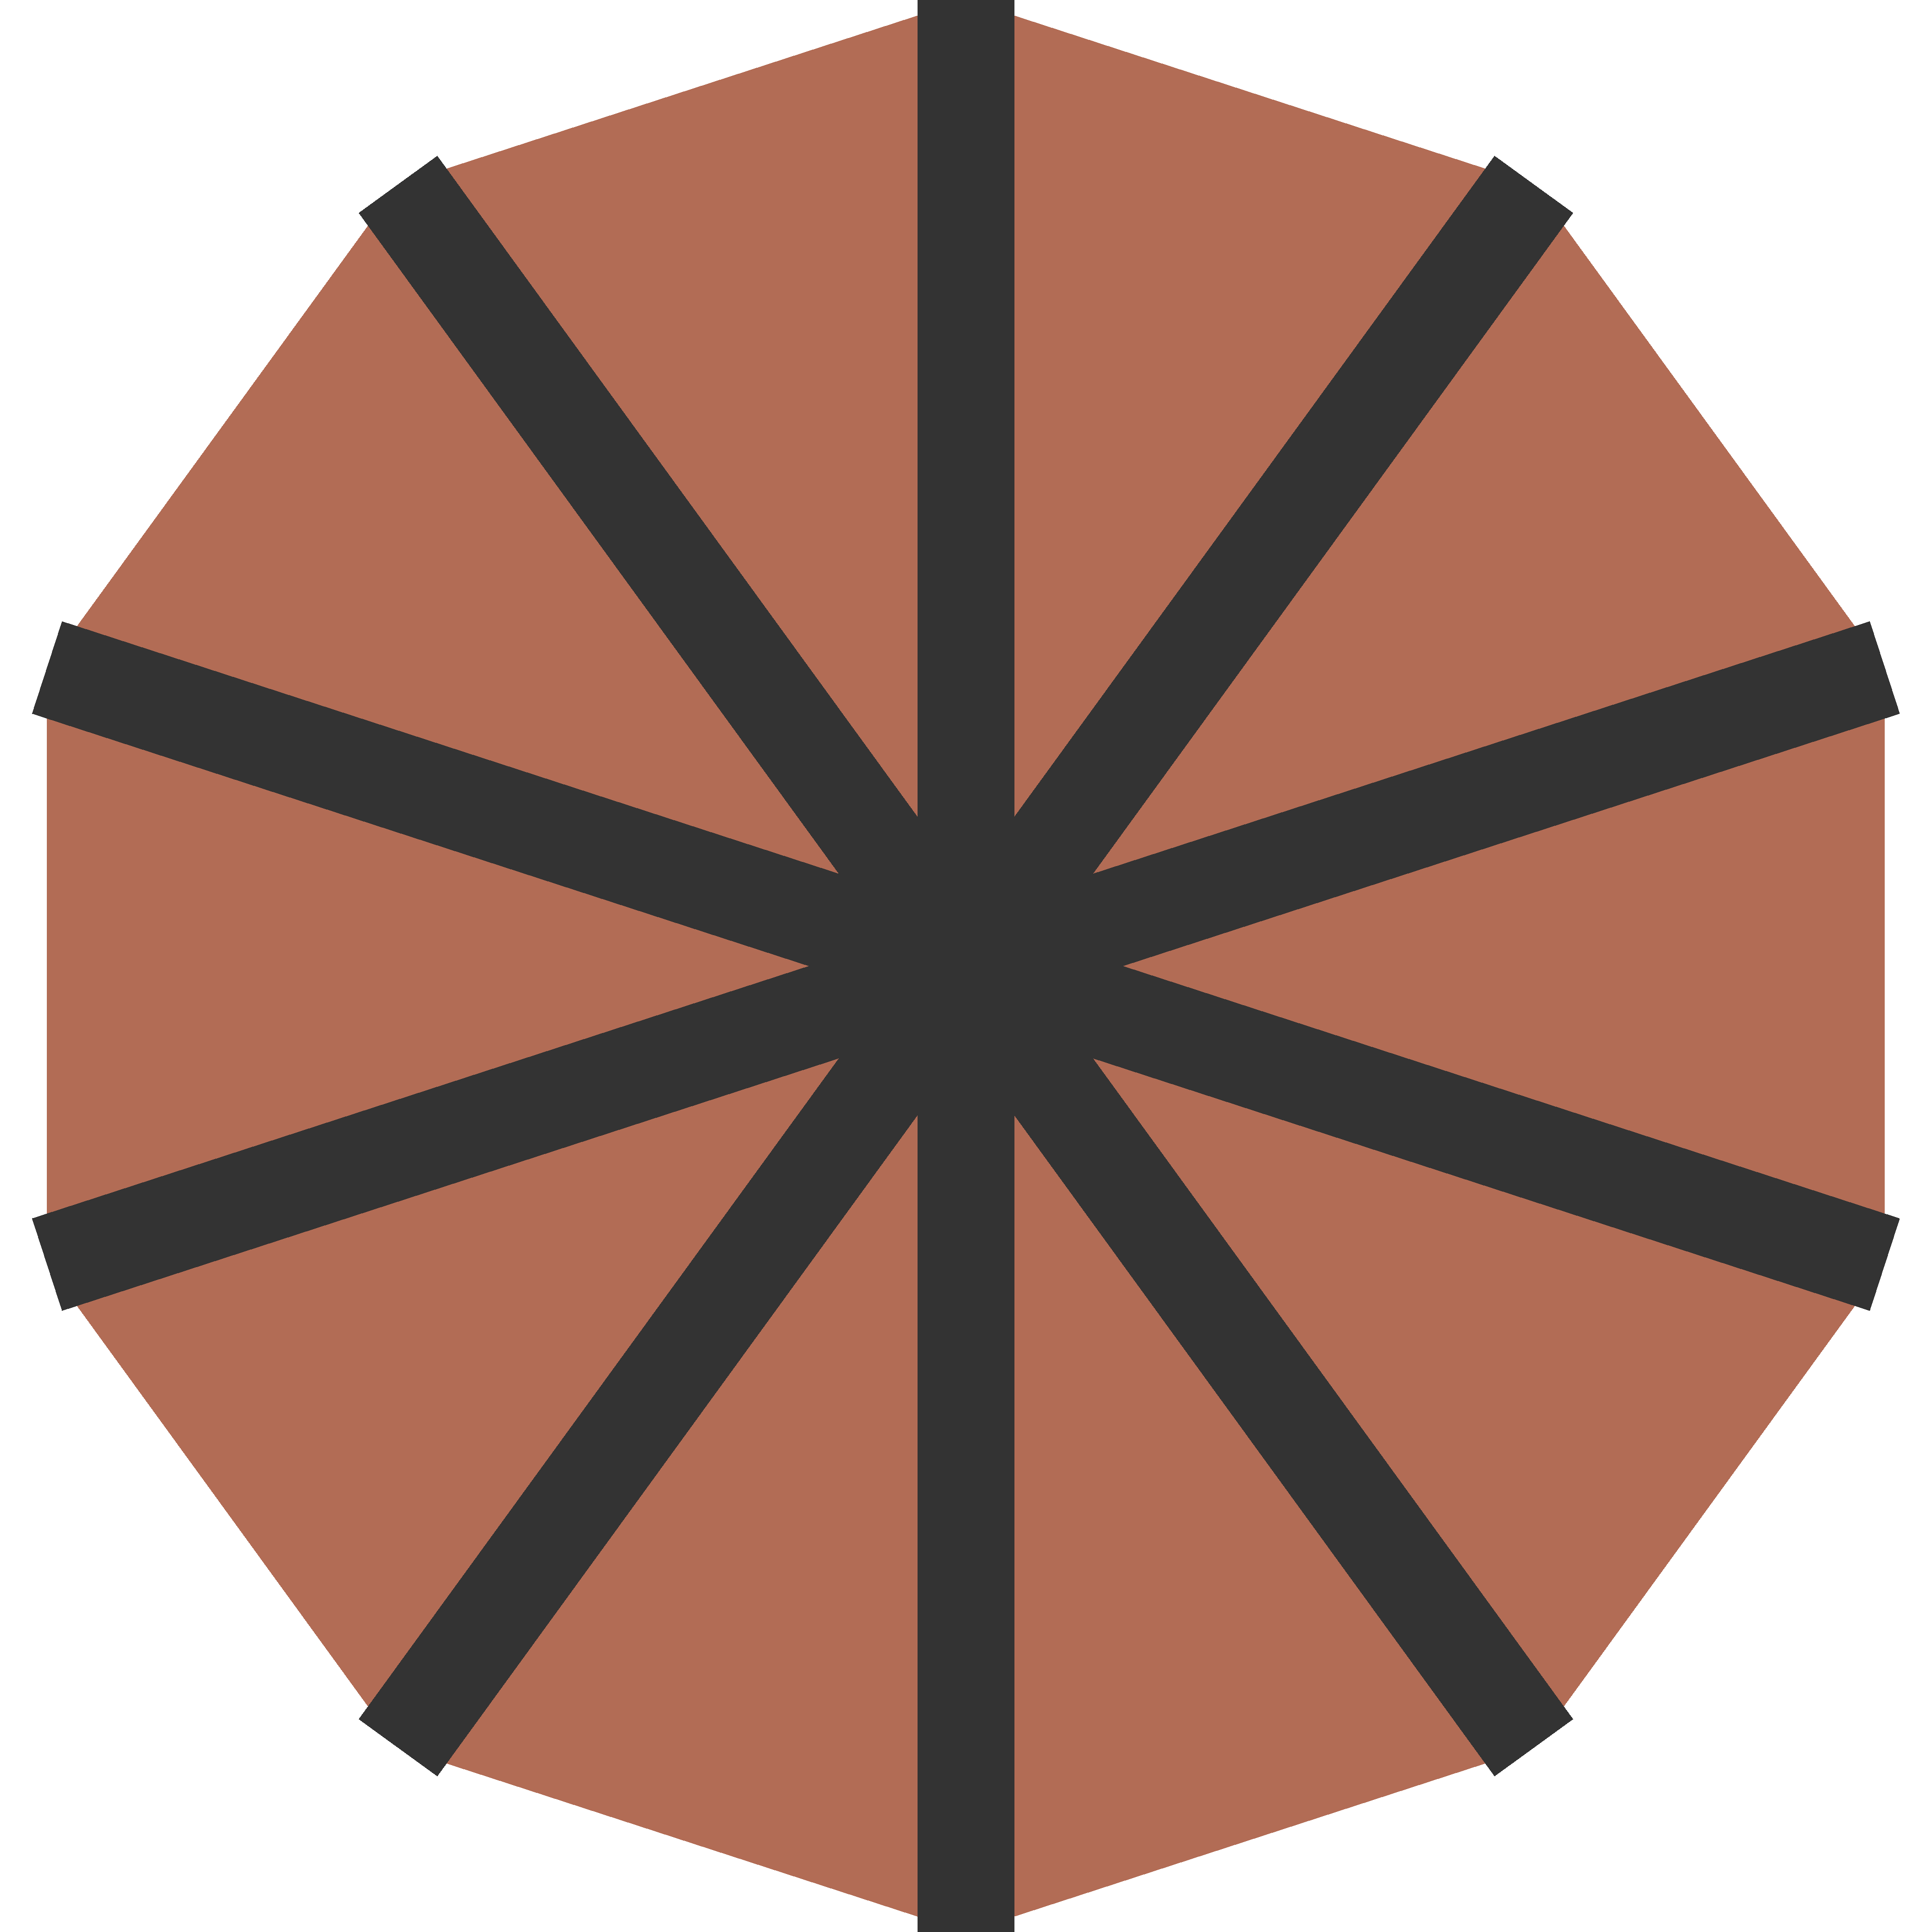
\includegraphics[width=0.9\textwidth]{img/wheel_P3_0.pdf}
\>
\<{6cm}

\includegraphics[width=0.9\textwidth]{img/wheel_P3_1.pdf}
\>
\)
}
\only<2>{
\(
\<{6cm}

\includegraphics[width=0.9\textwidth]{img/wheel_P3_1.pdf}
\>
\<{6cm}

\includegraphics[width=0.9\textwidth]{img/wheel_P3_2.pdf}
\>
\)
}
\only<3>{
\(
\<{6cm}

\includegraphics[width=0.9\textwidth]{img/wheel_P3_2.pdf}
\>
\<{6cm}

\includegraphics[width=0.9\textwidth]{img/wheel_P3_3.pdf}
\>
\)
}
\only<4>{
\(
\<{6cm}

\includegraphics[width=0.9\textwidth]{img/wheel_P3_3.pdf}
\>
\<{6cm}
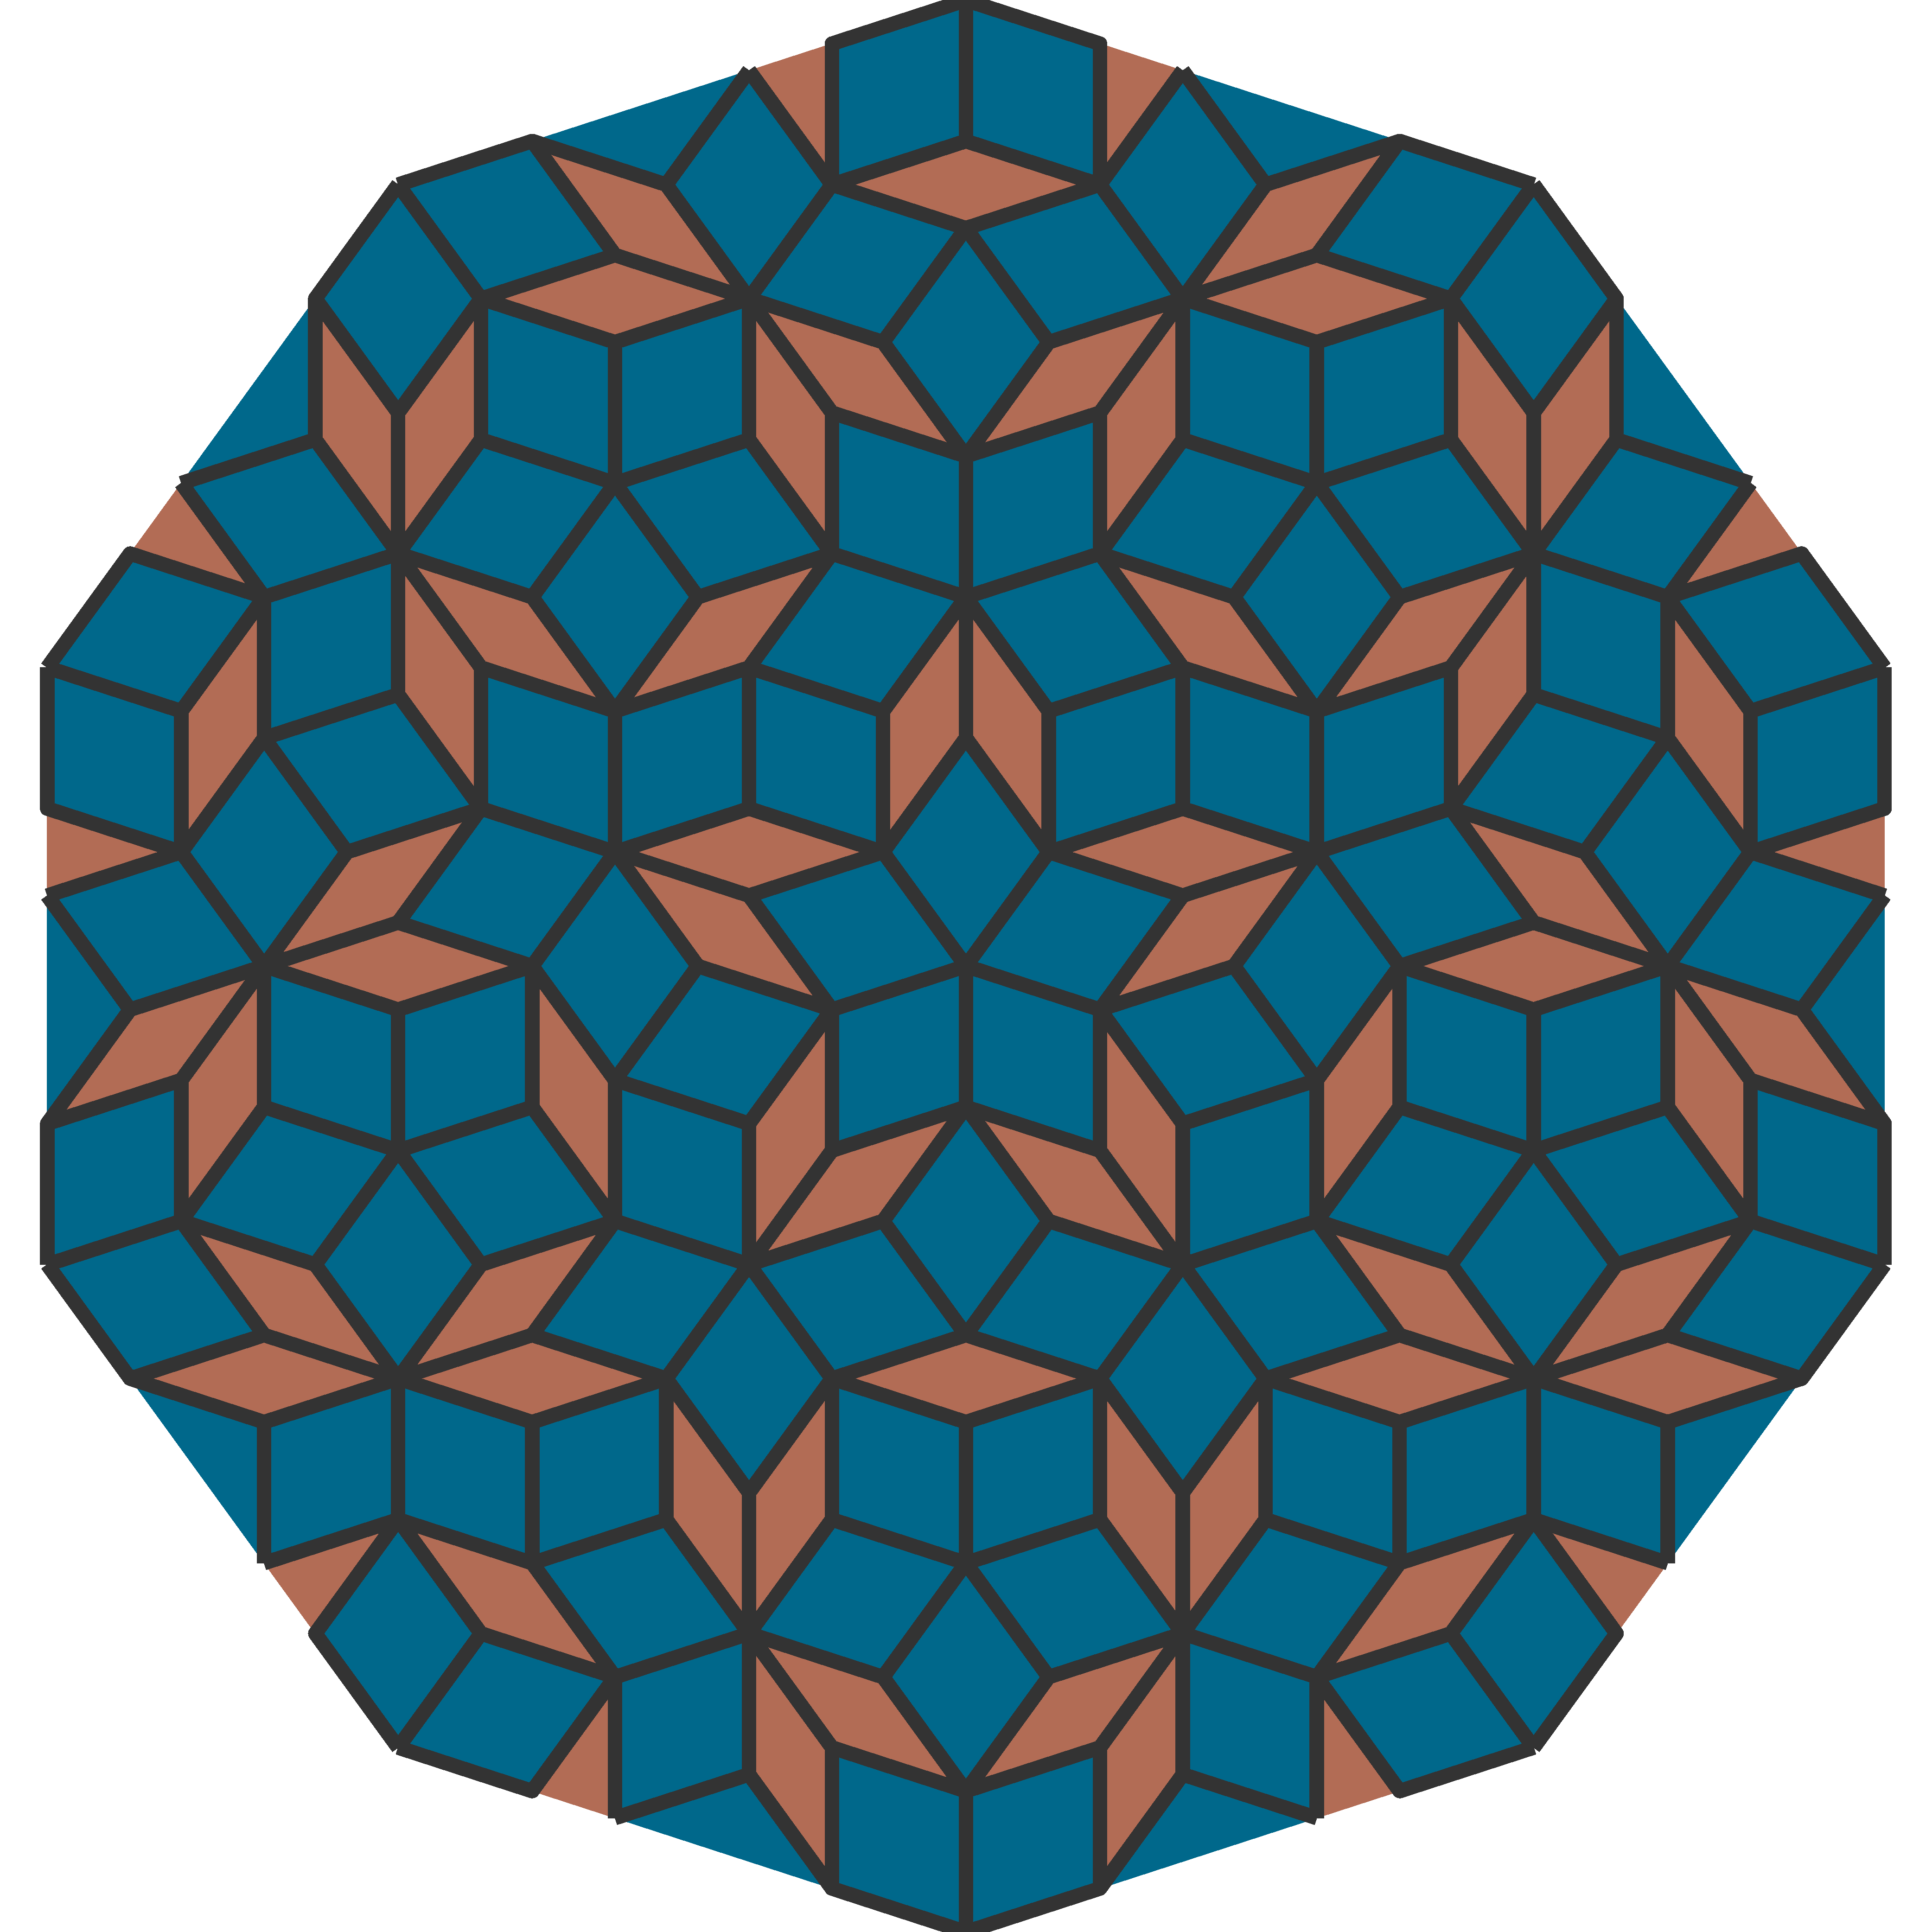
\includegraphics[width=0.9\textwidth]{img/wheel_P3_4.pdf}
\>
\)
}
\only<5>{
\(
\<{6cm}
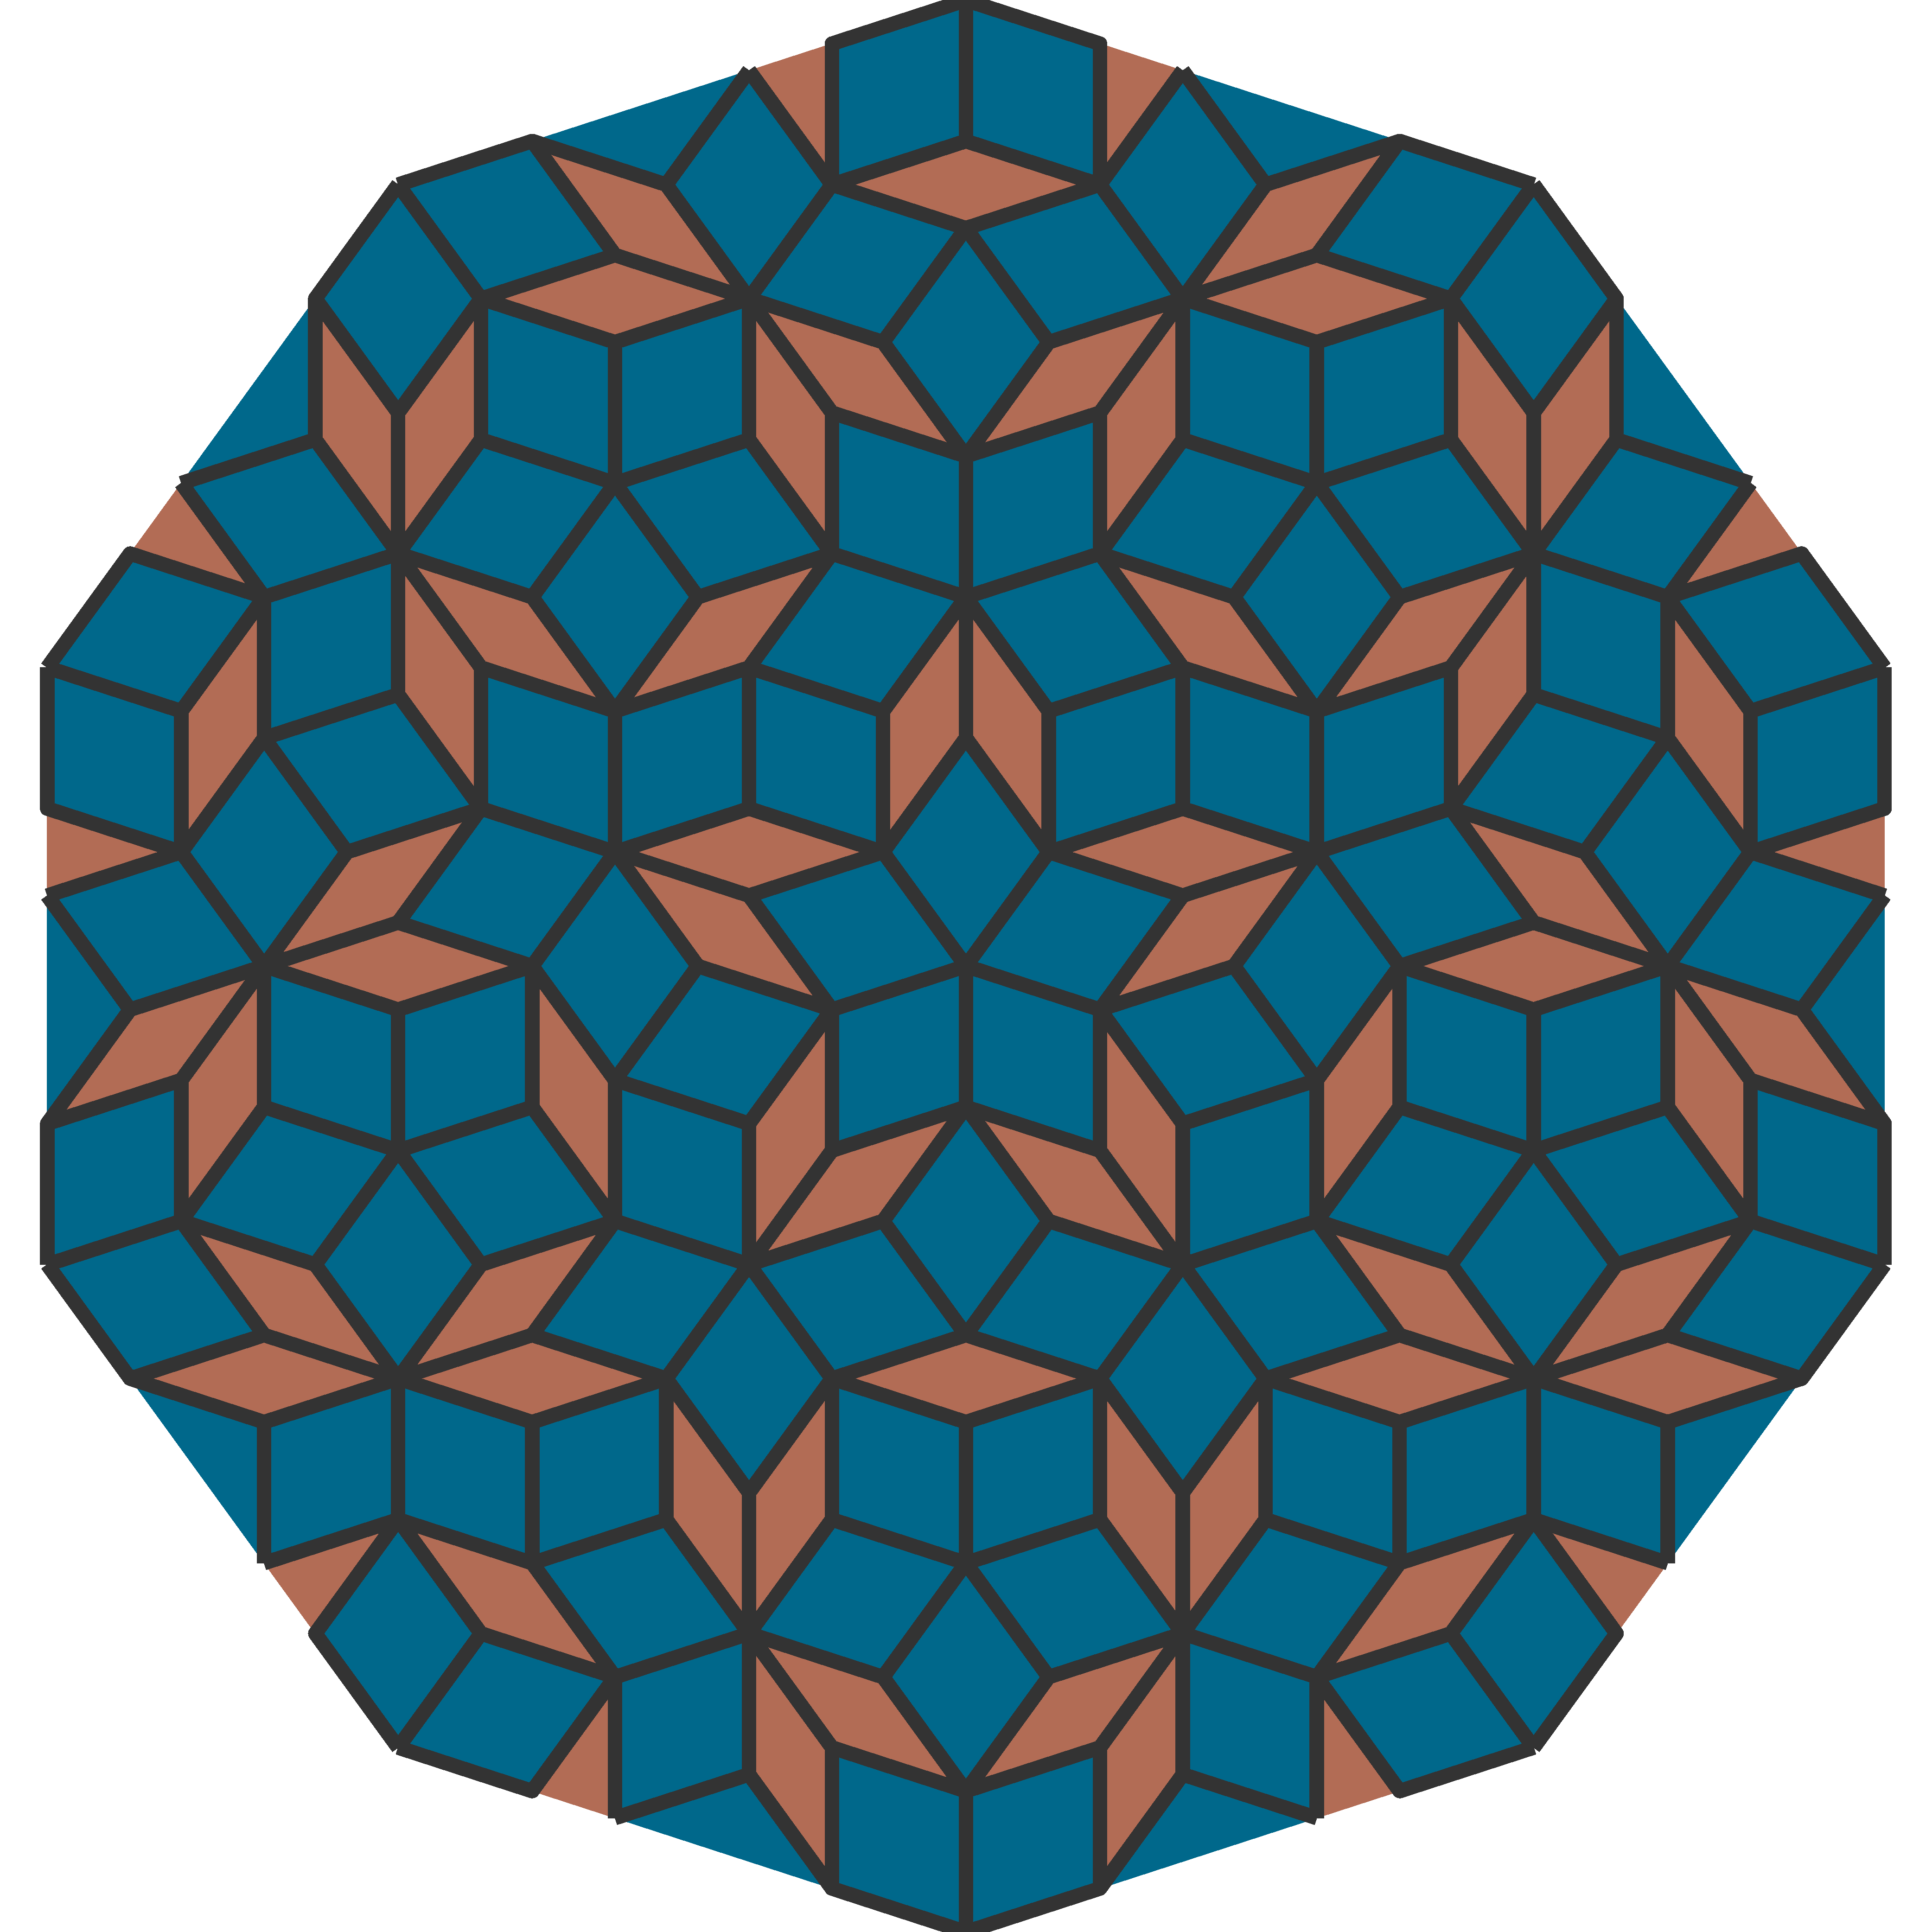
\includegraphics[width=0.9\textwidth]{img/wheel_P3_4.pdf}
\>
\<{6cm}
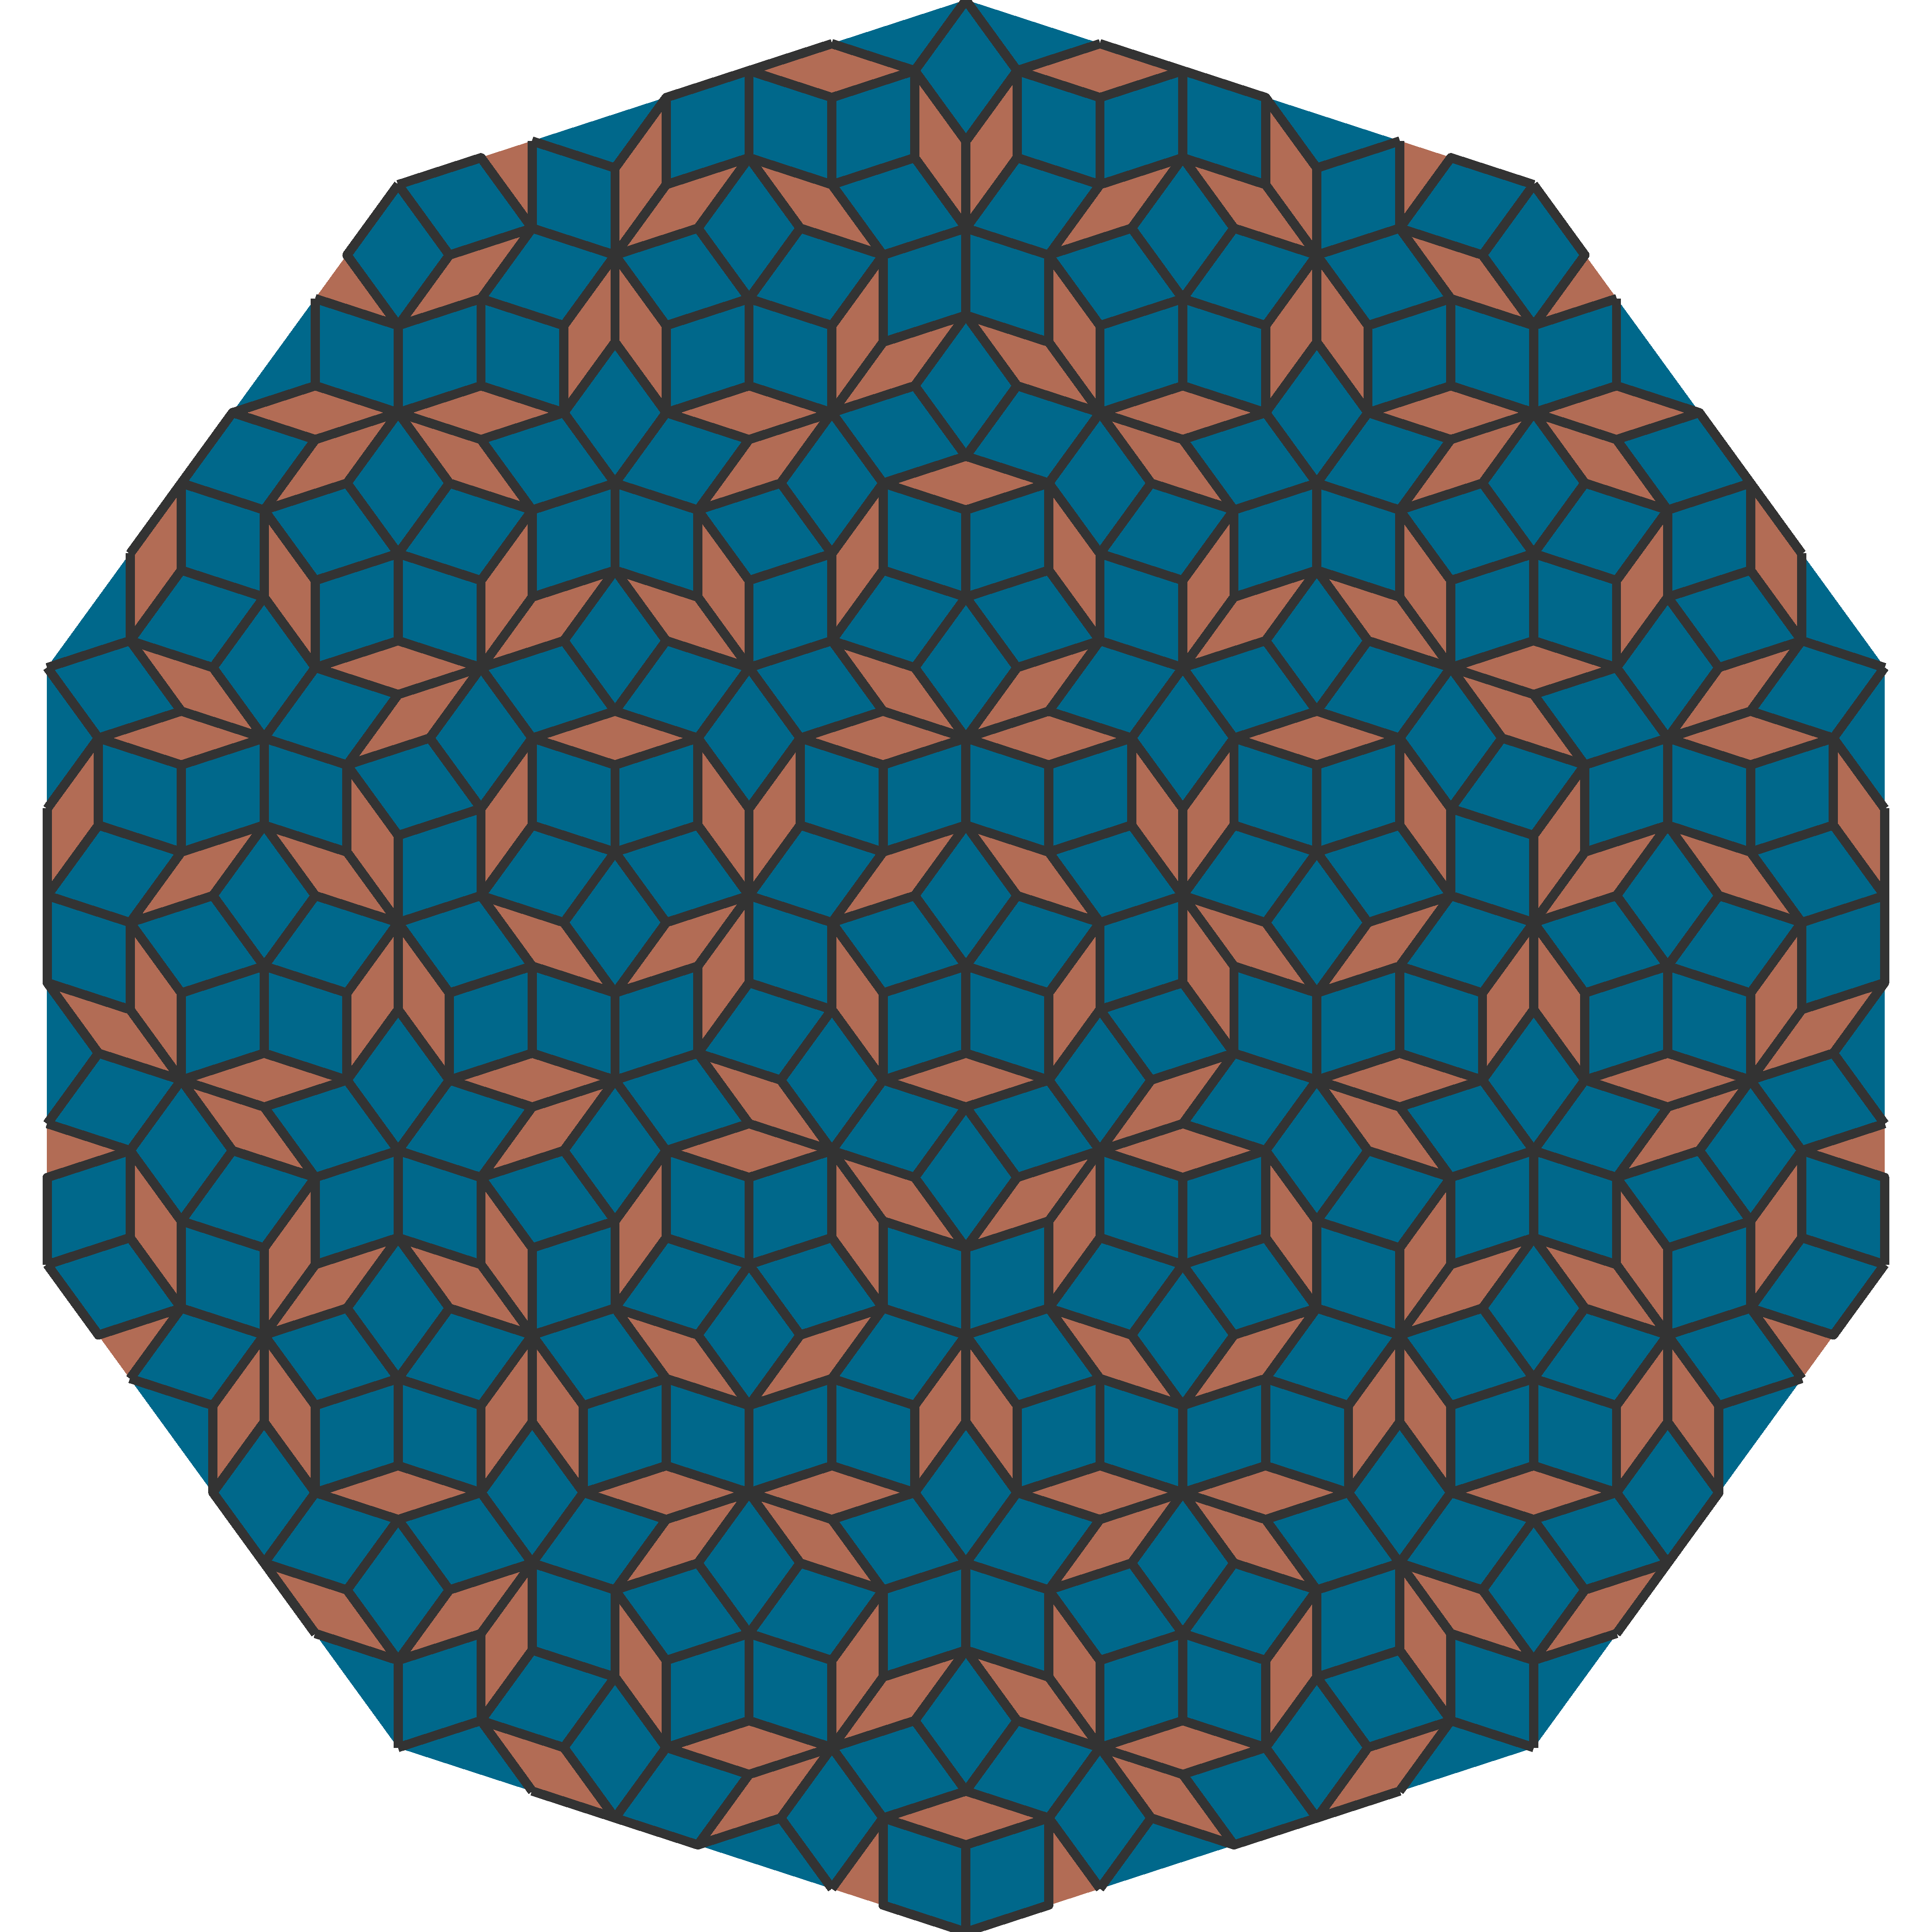
\includegraphics[width=0.9\textwidth]{img/wheel_P3_5.pdf}
\>
\)
}
\end{frame}

\begin{frame}{L'inflation et les choux romanesco}
\centering
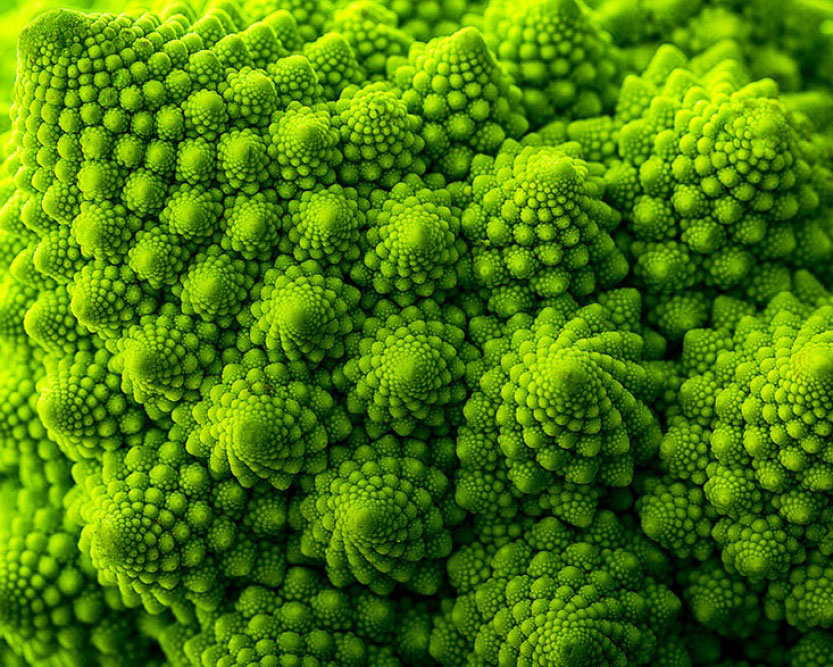
\includegraphics[width=.8\textwidth]{img/chou_romanesco.jpg}
\end{frame}

\section{Un peu de physique}
\subsection{Dummy}
\begin{frame}{Où sont les atomes ?}
\centering

\includegraphics[width=0.6\textwidth]{img/wheel_P3_2_atoms.pdf}
\end{frame}

\begin{frame}{Densité électronique}
{\centering
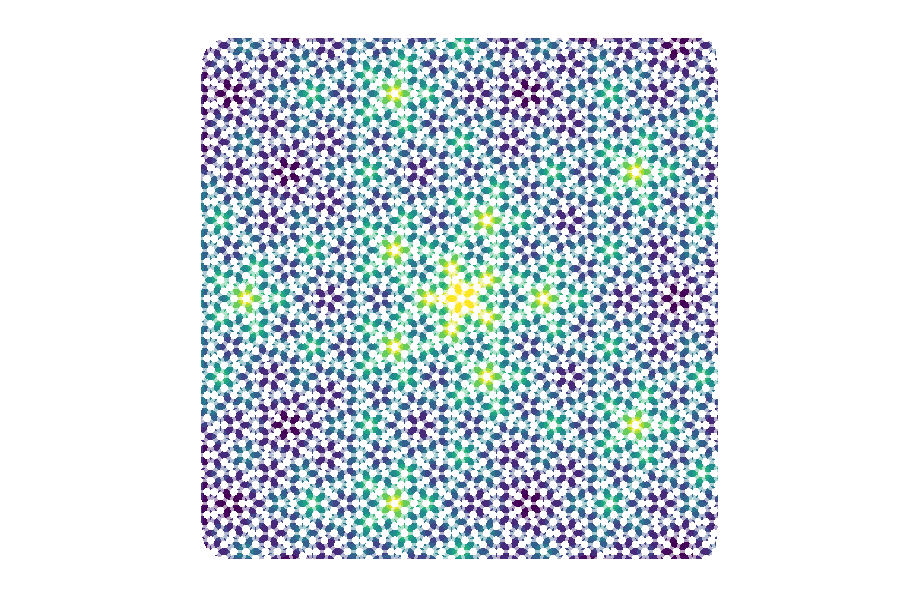
\includegraphics[width=.9\textwidth]{img/electronic_density.pdf}

}

Basé sur des travaux de Bill Sutherland (1986).
\end{frame}

\begin{frame}{Densité électronique (bis)}
\(
\<{6cm}
\centering
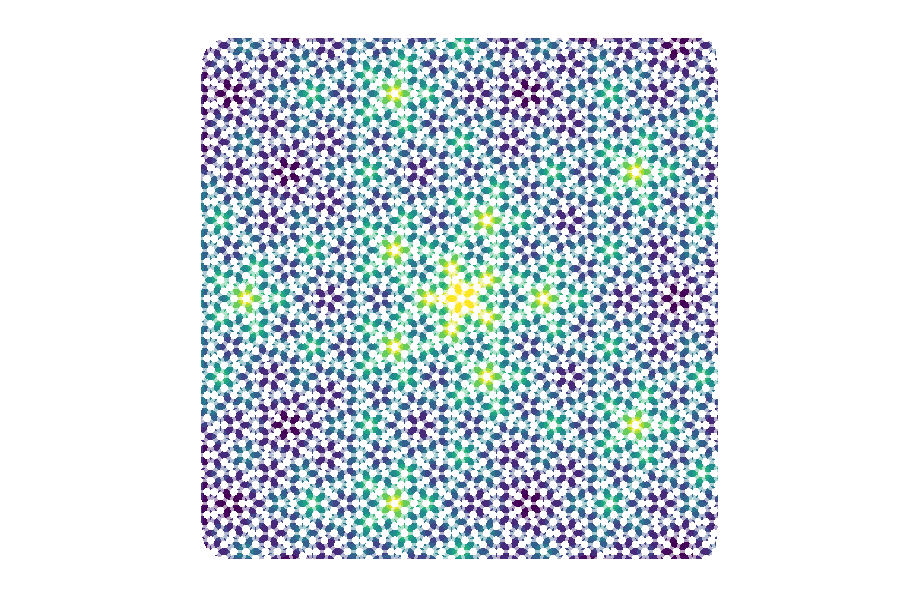
\includegraphics[width=0.9\textwidth]{img/electronic_density.pdf}
\>
\<{6cm}
\centering
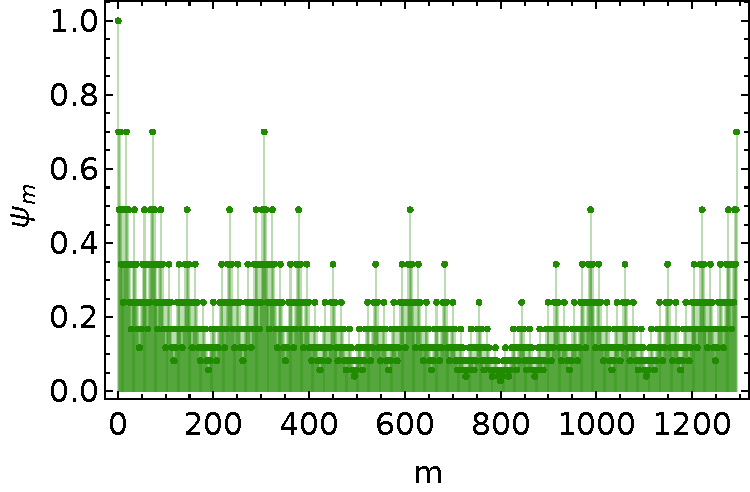
\includegraphics[width=0.9\textwidth]{img/wf.pdf}%

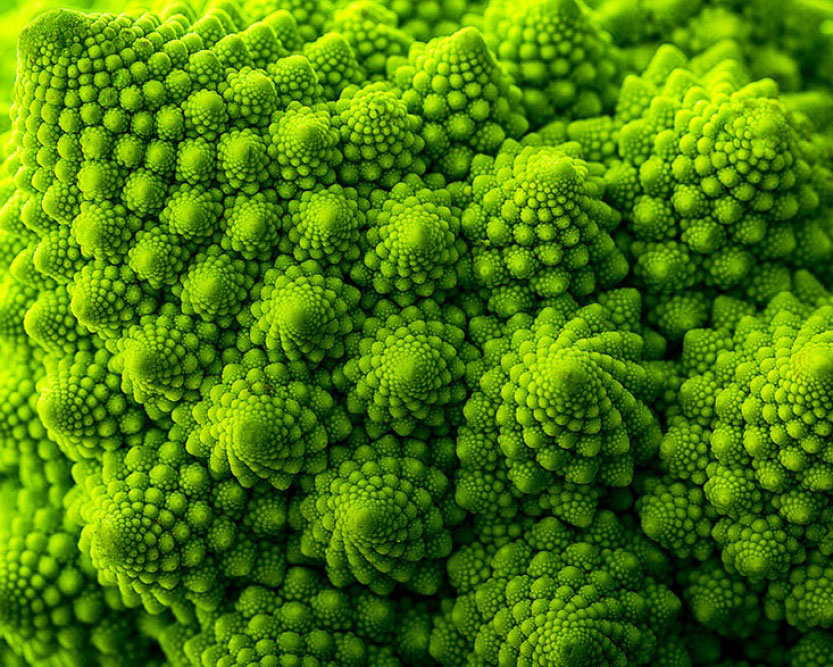
\includegraphics[width=.8\textwidth]{img/chou_romanesco.jpg}
\>
\)
\end{frame}

\section{Des dimensions supplémentaires}
\subsection{Dummy}

\begin{frame}{Pavage de Rauzy}
{\centering
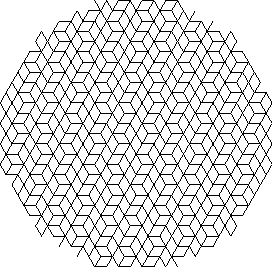
\includegraphics[width=0.6\textwidth]{img/rauzy.pdf}

}

Tiré de : \emph{Hofstadter butterfly of a quasicrystal, Fuchs \& Vidal}.
\end{frame}

\begin{frame}{Pavage d'Ammann-Beenker}
\centering

\includegraphics[width=0.9\textwidth]{img/AB_tiling_patch.pdf}

\only<2>{
Projection de cubes en 4 dimensions!
}
\end{frame}

\begin{frame}{Pavage de Penrose}
\centering
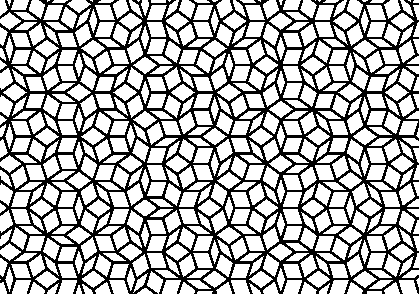
\includegraphics[width=0.9\textwidth]{img/Penrose_tiling_cropped.pdf}

\only<2>{
Projection de cubes en 5 dimensions!
}
\end{frame}

\section{Misc}
\subsection{Dummy}

\begin{frame}{Règles d'inflation pour les demi-tuiles}
\(
\<{6cm}
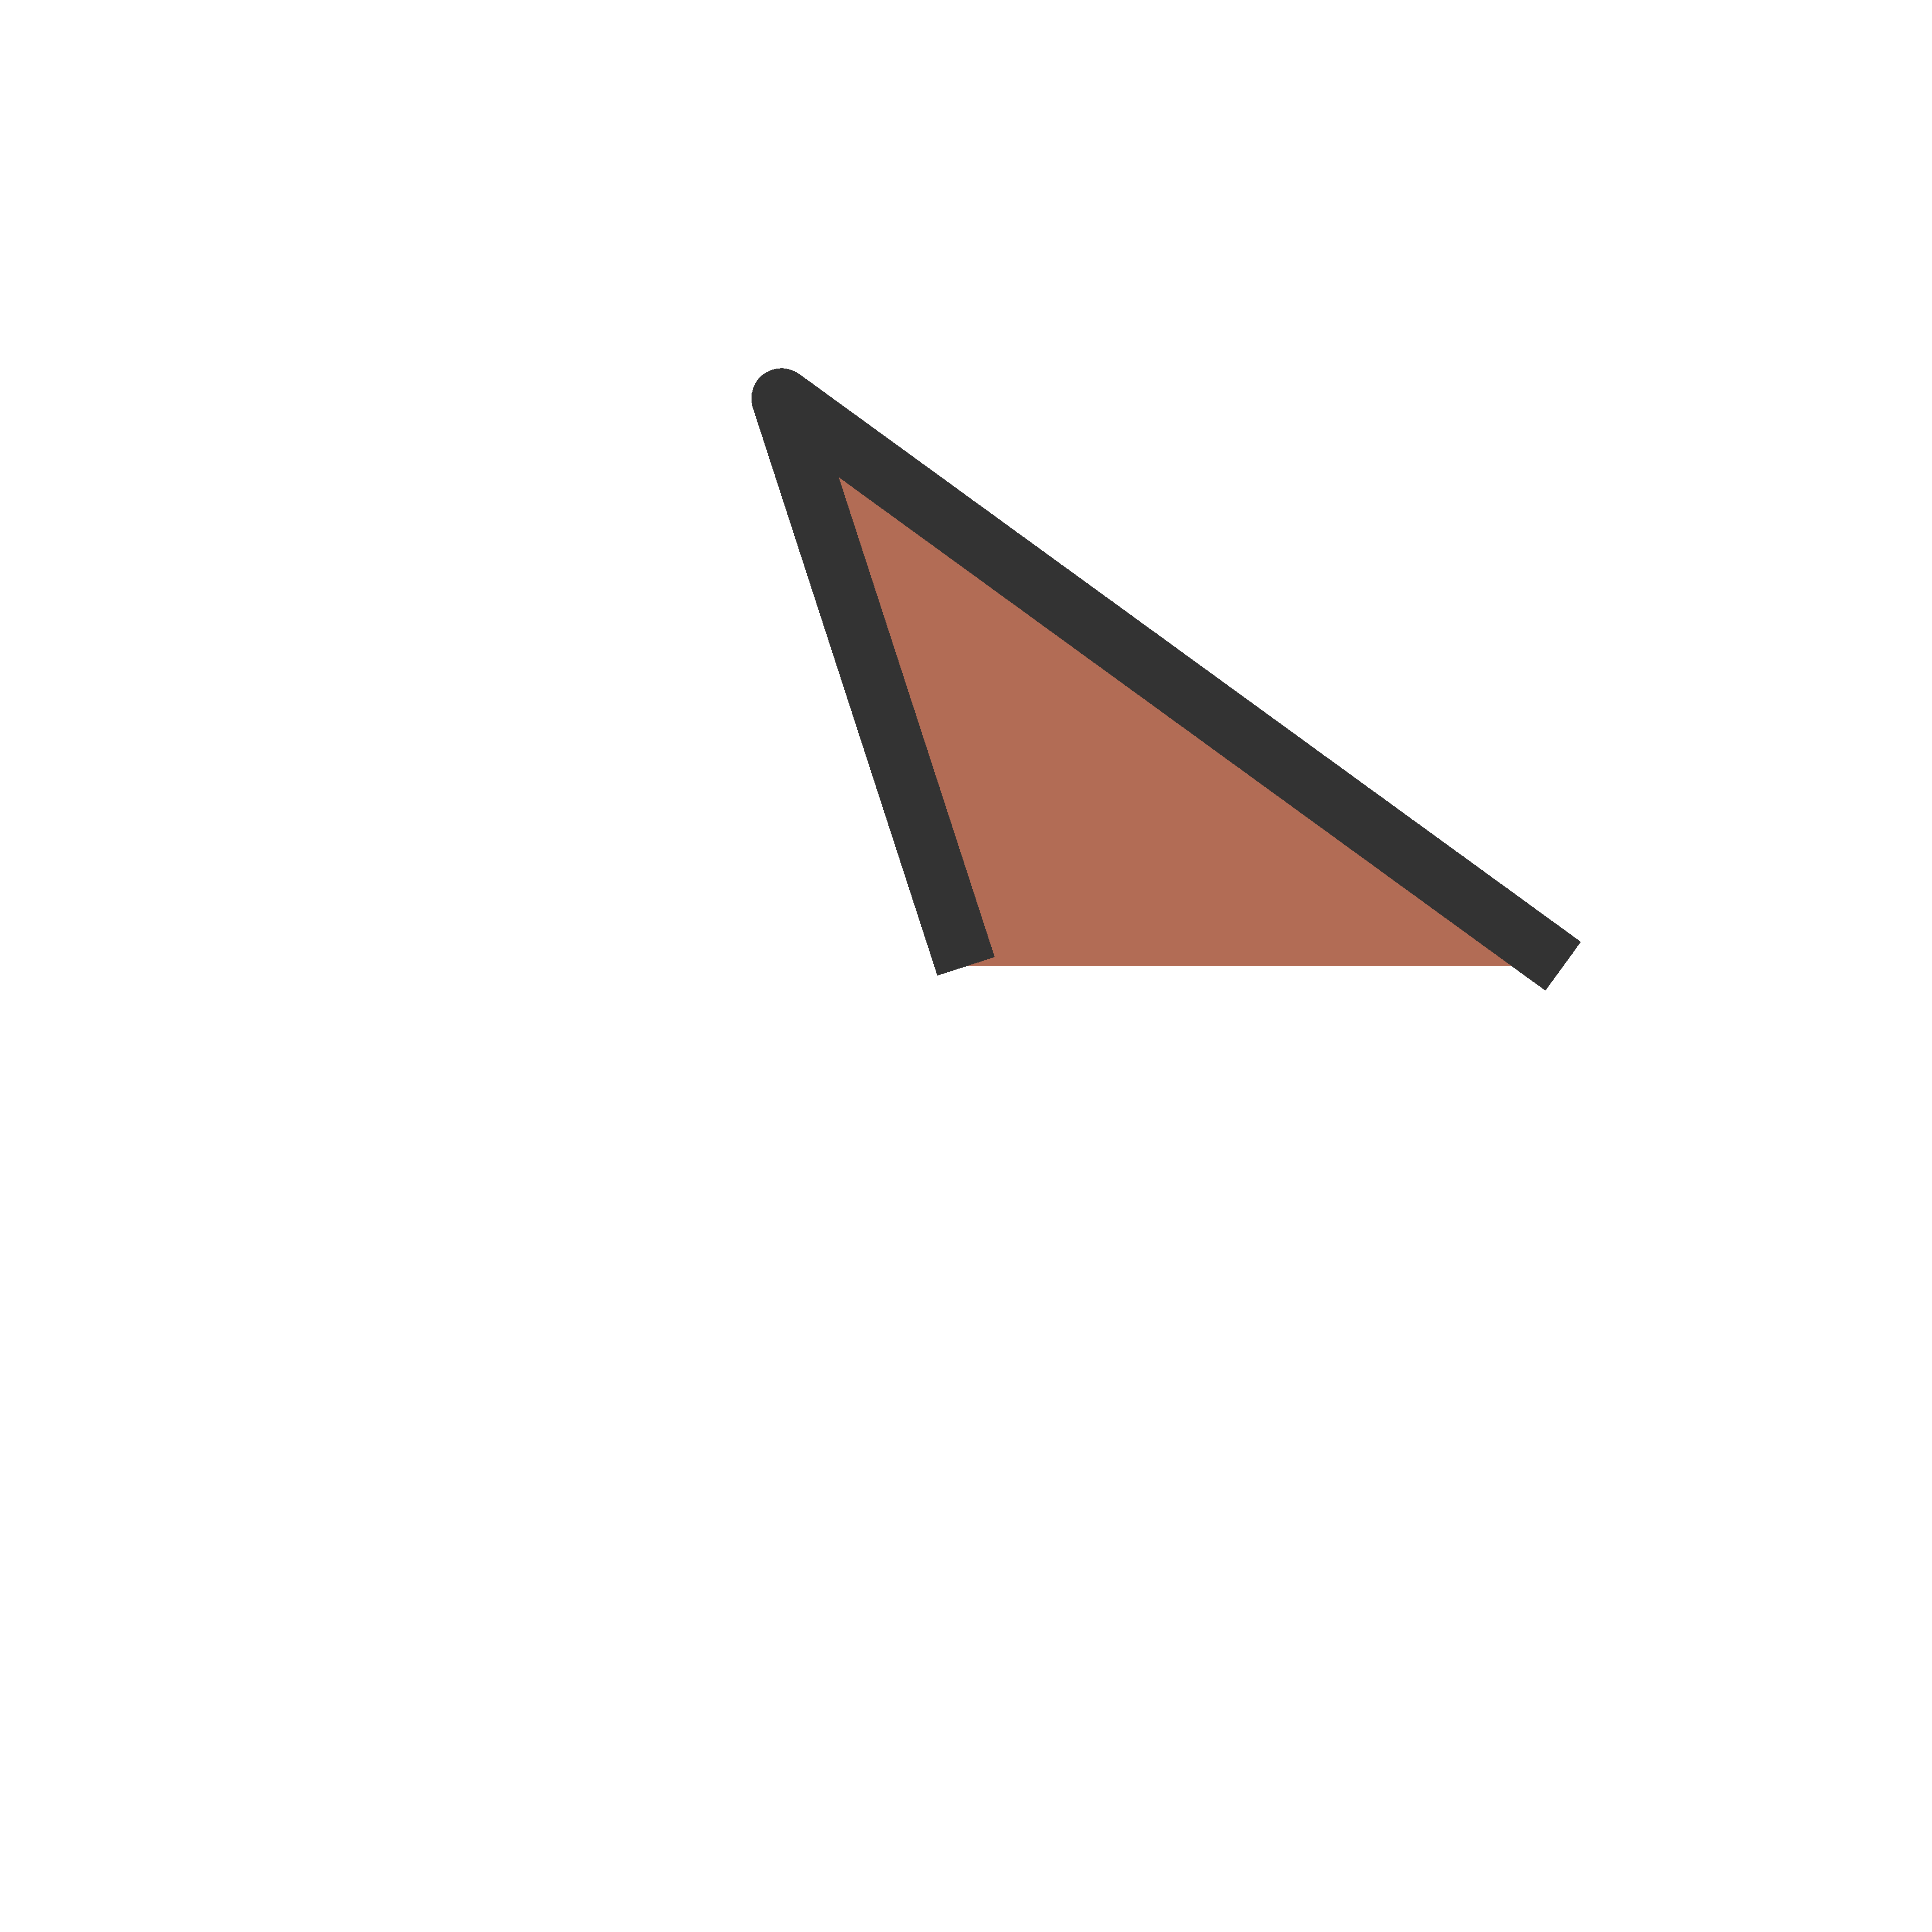
\includegraphics[width=0.8\textwidth]{img/dart.pdf} \\
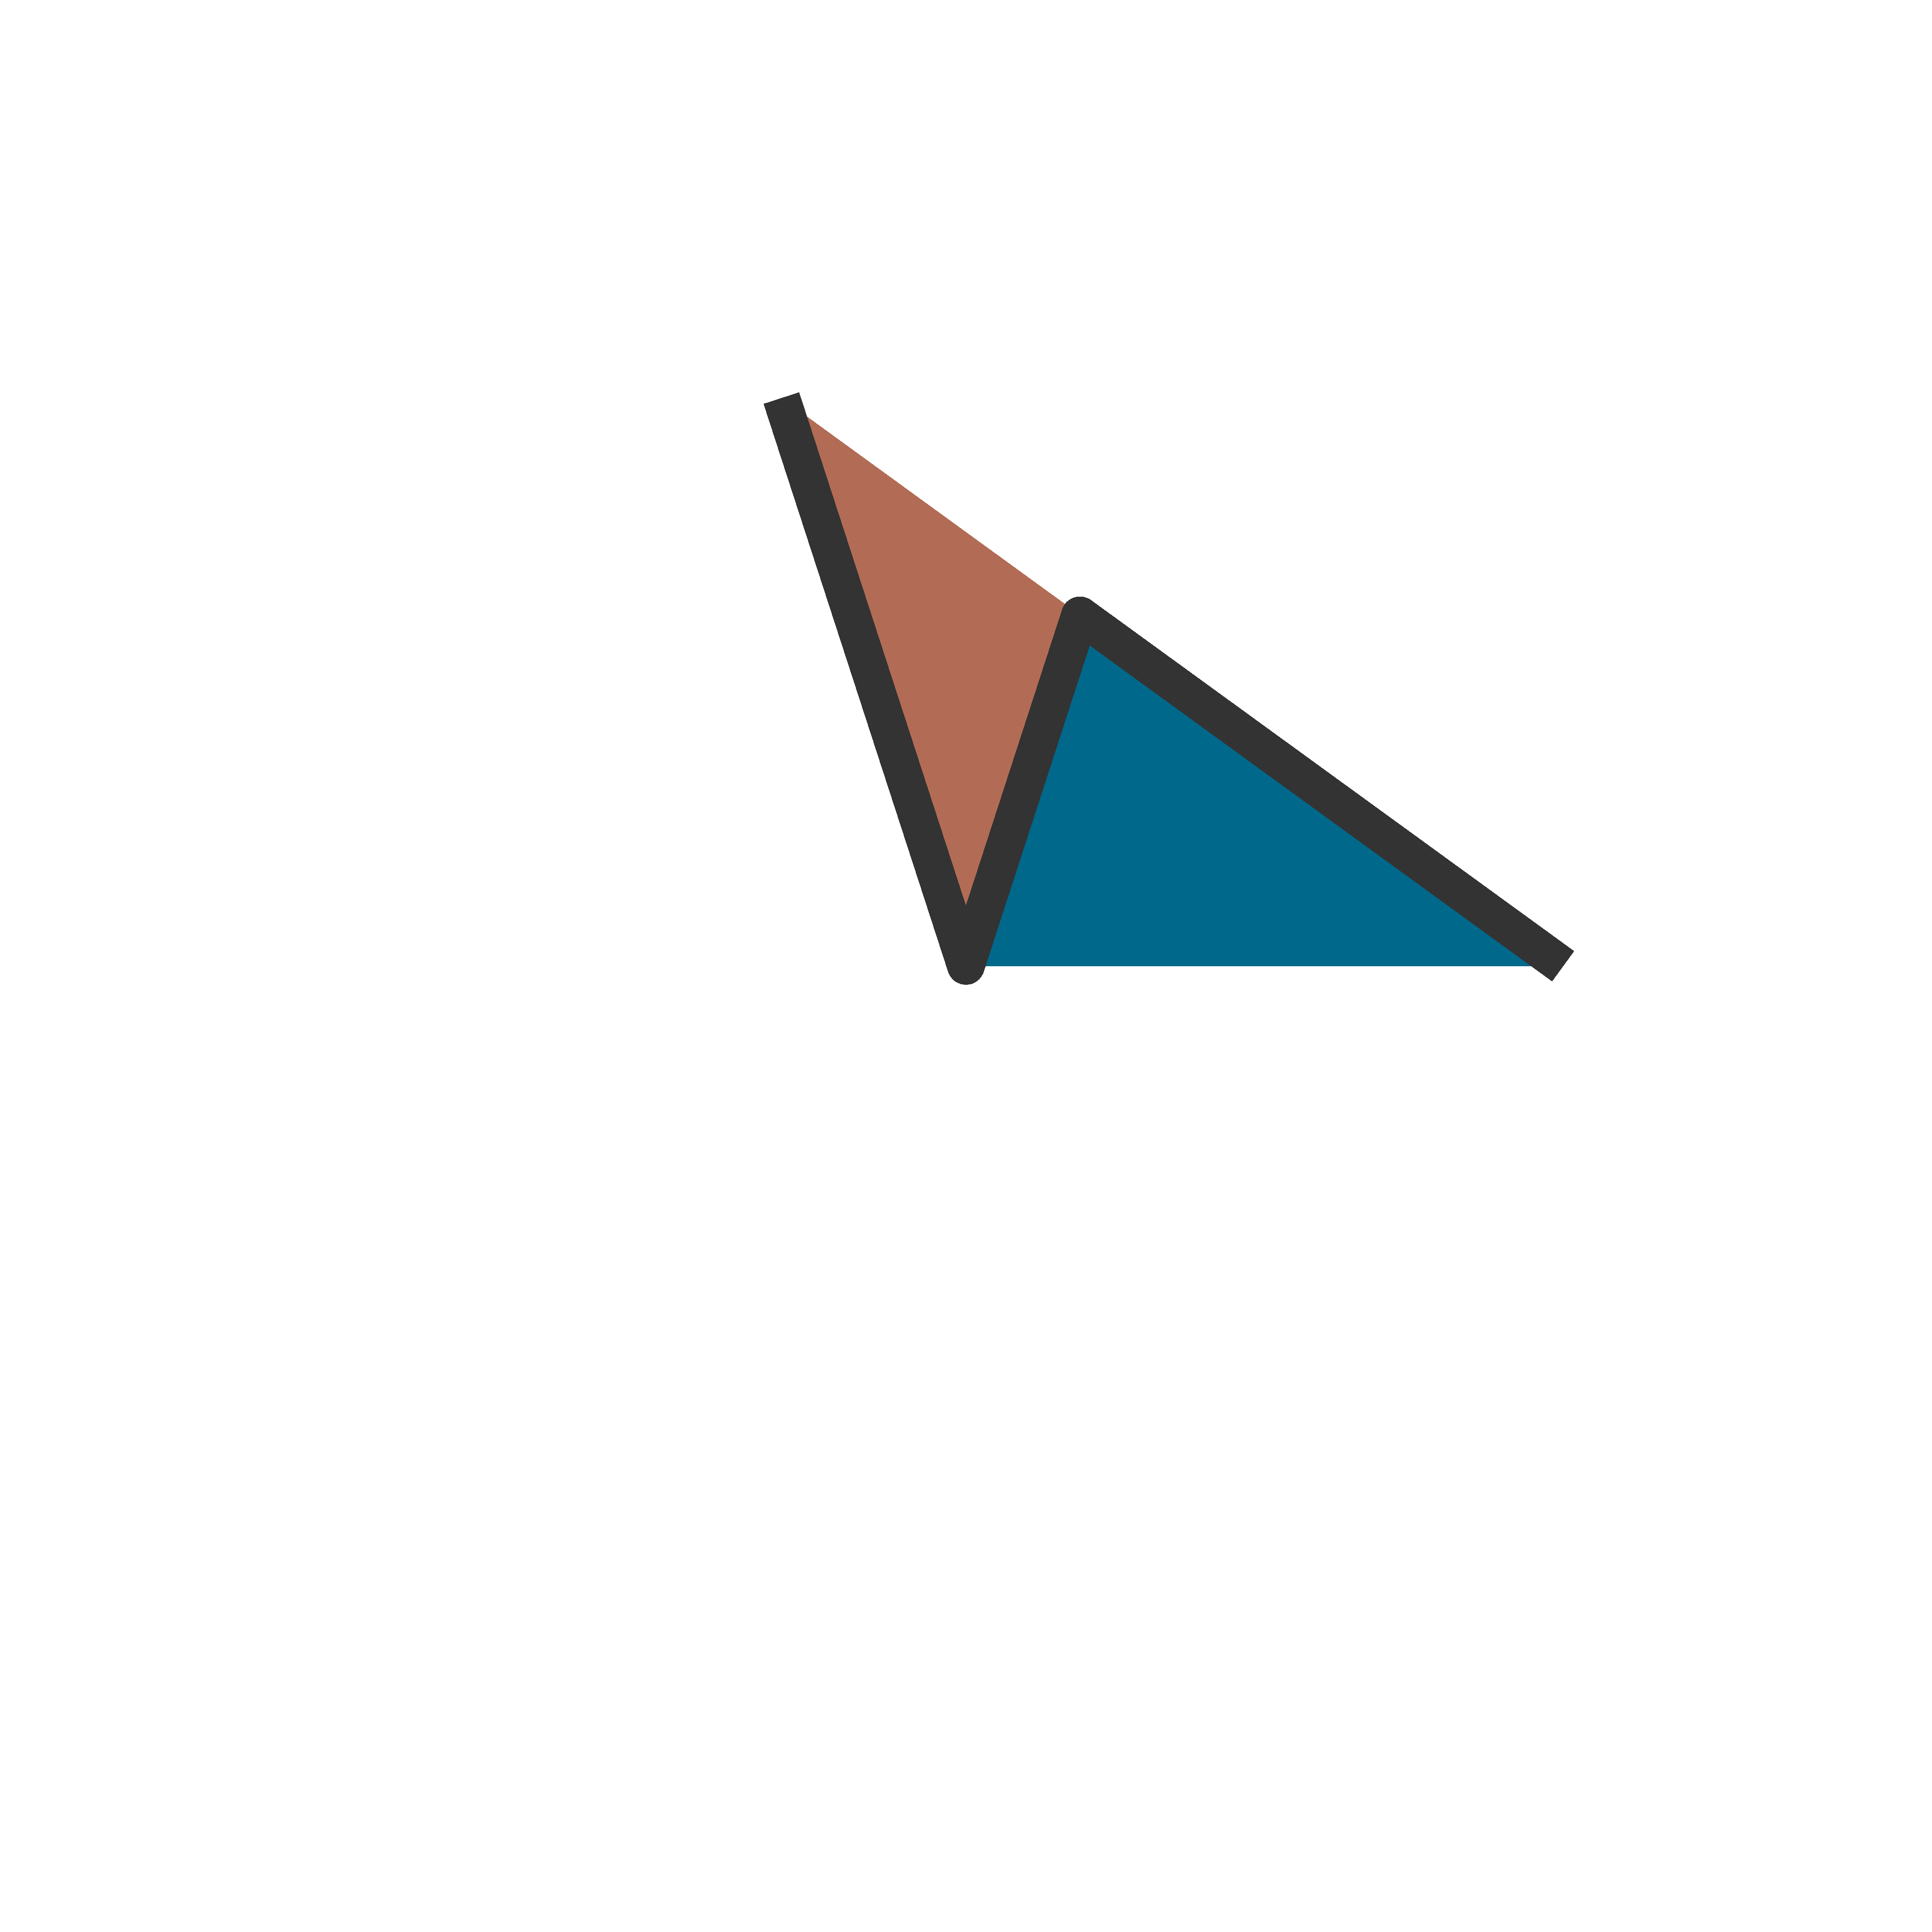
\includegraphics[width=0.8\textwidth]{img/dart_inflated.pdf}
\>
\<{6cm}
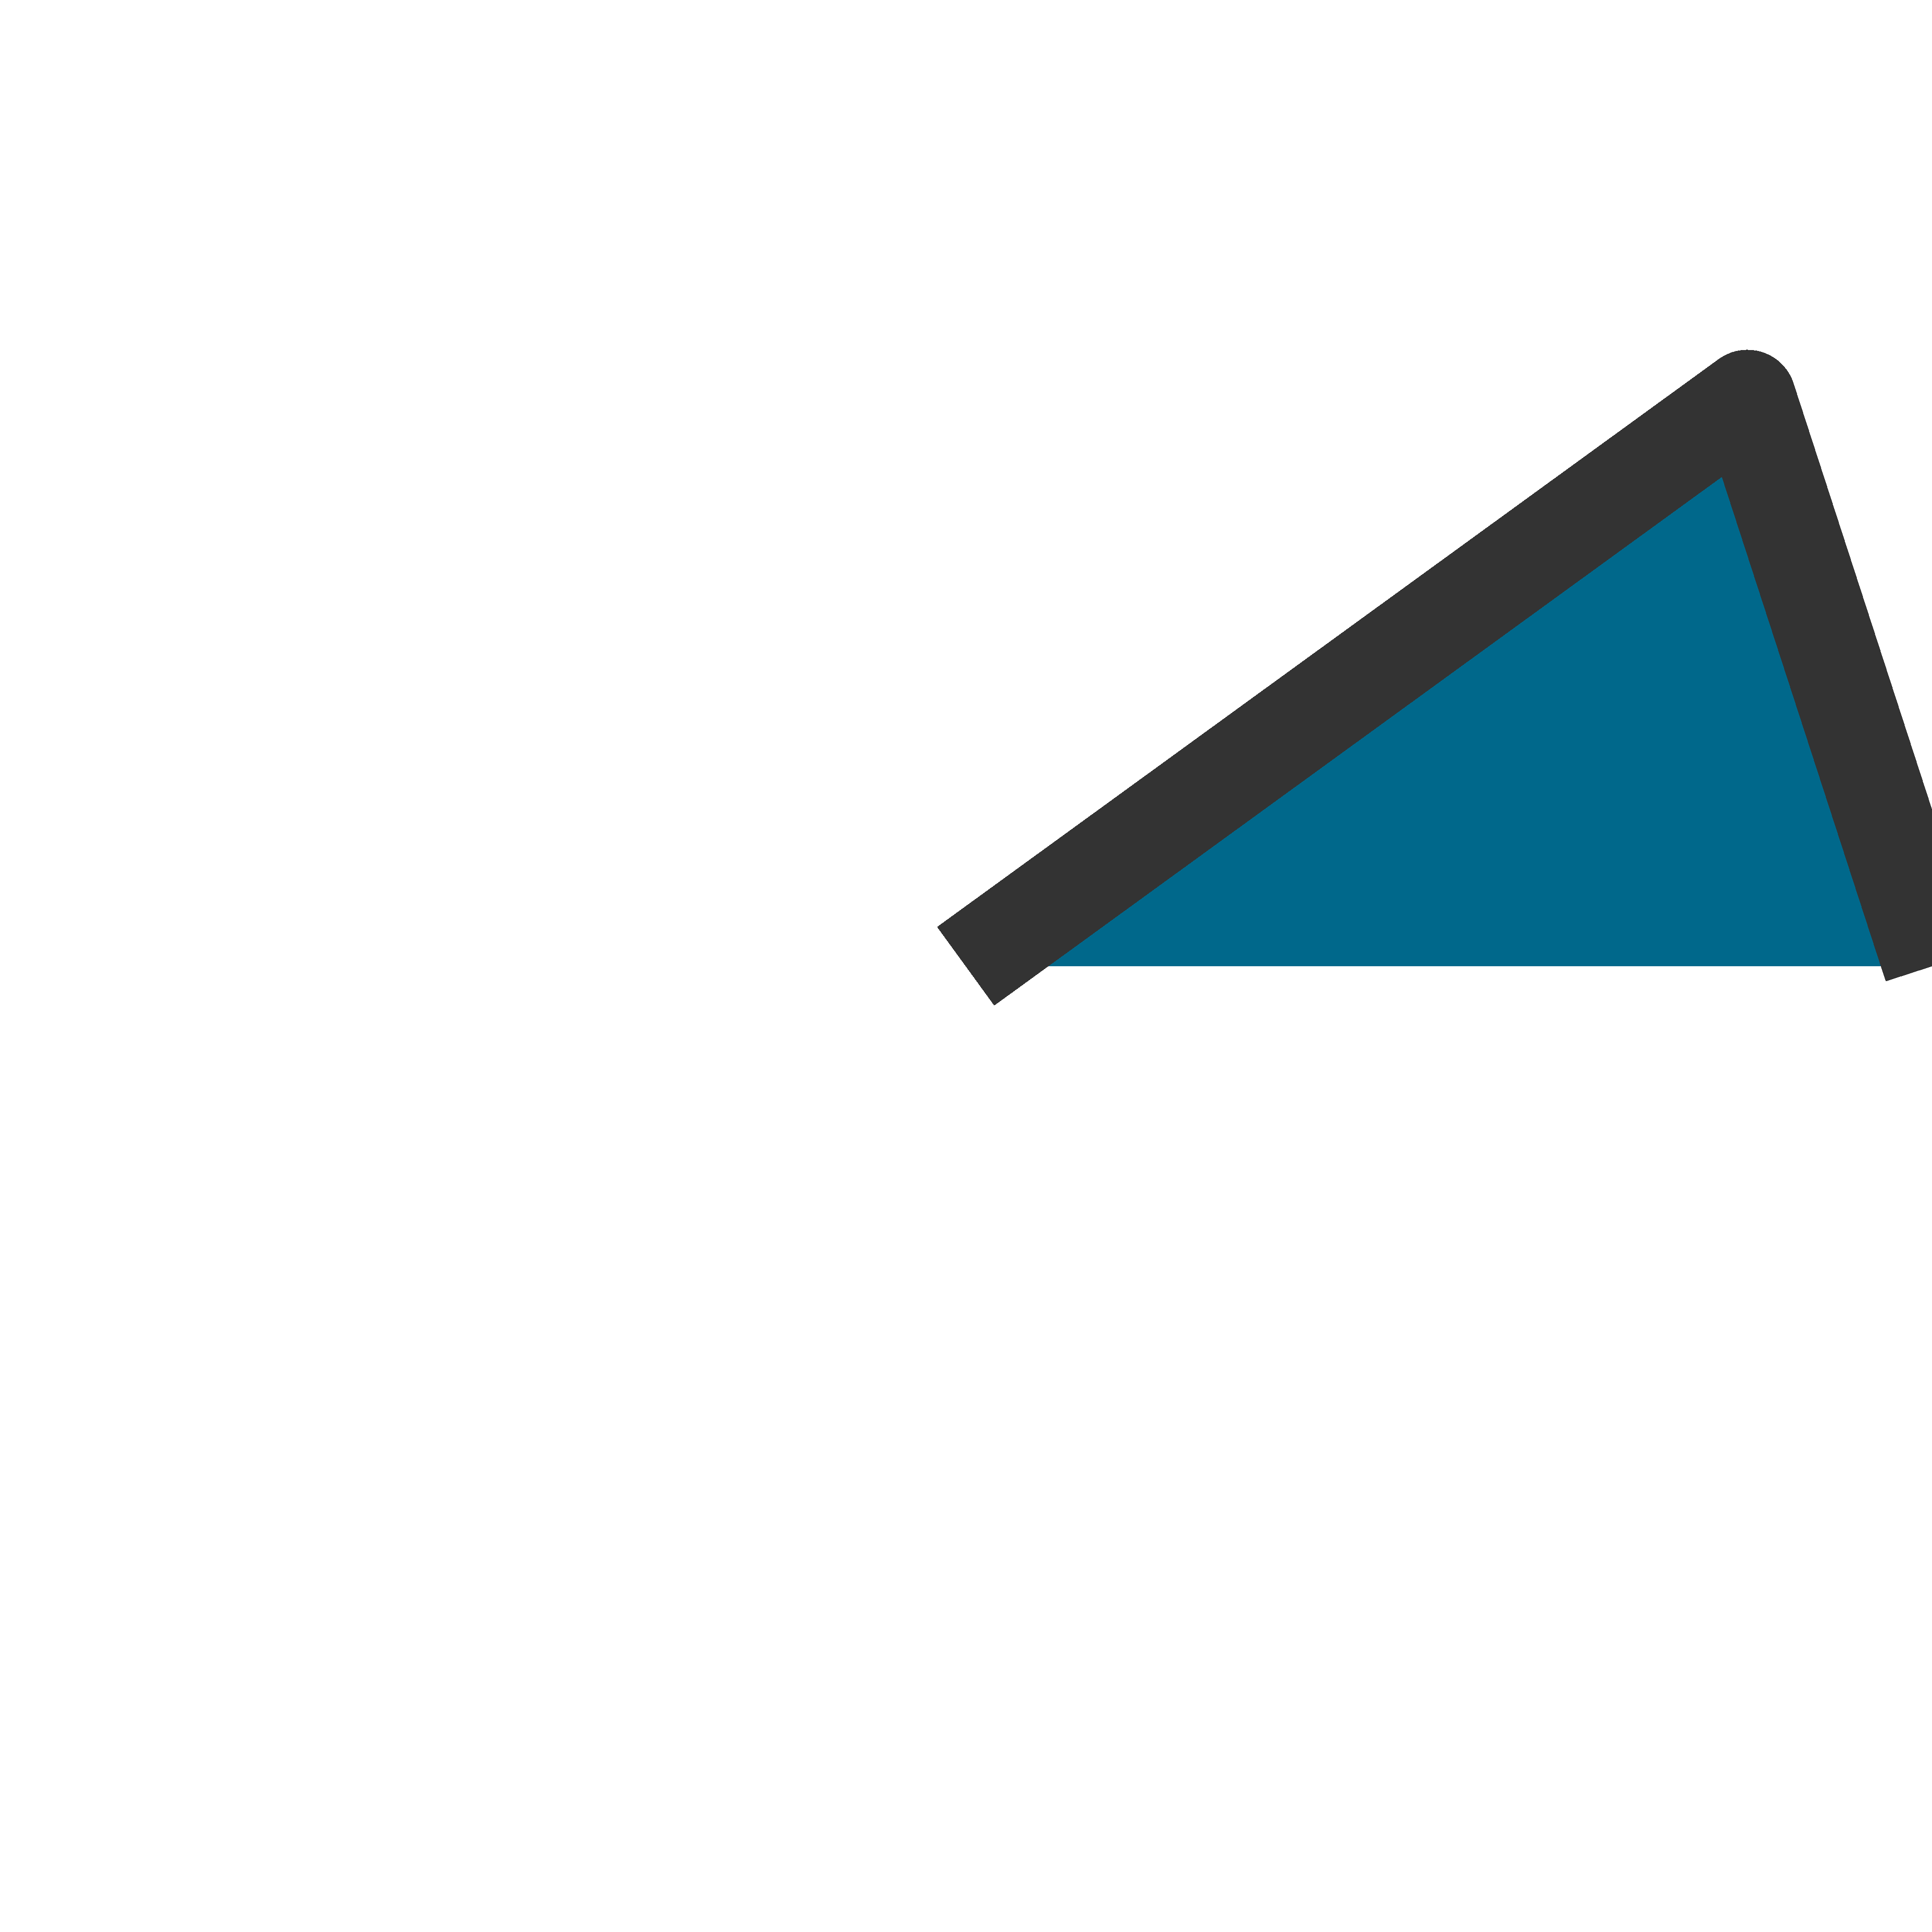
\includegraphics[width=0.8\textwidth]{img/kite.pdf} \\
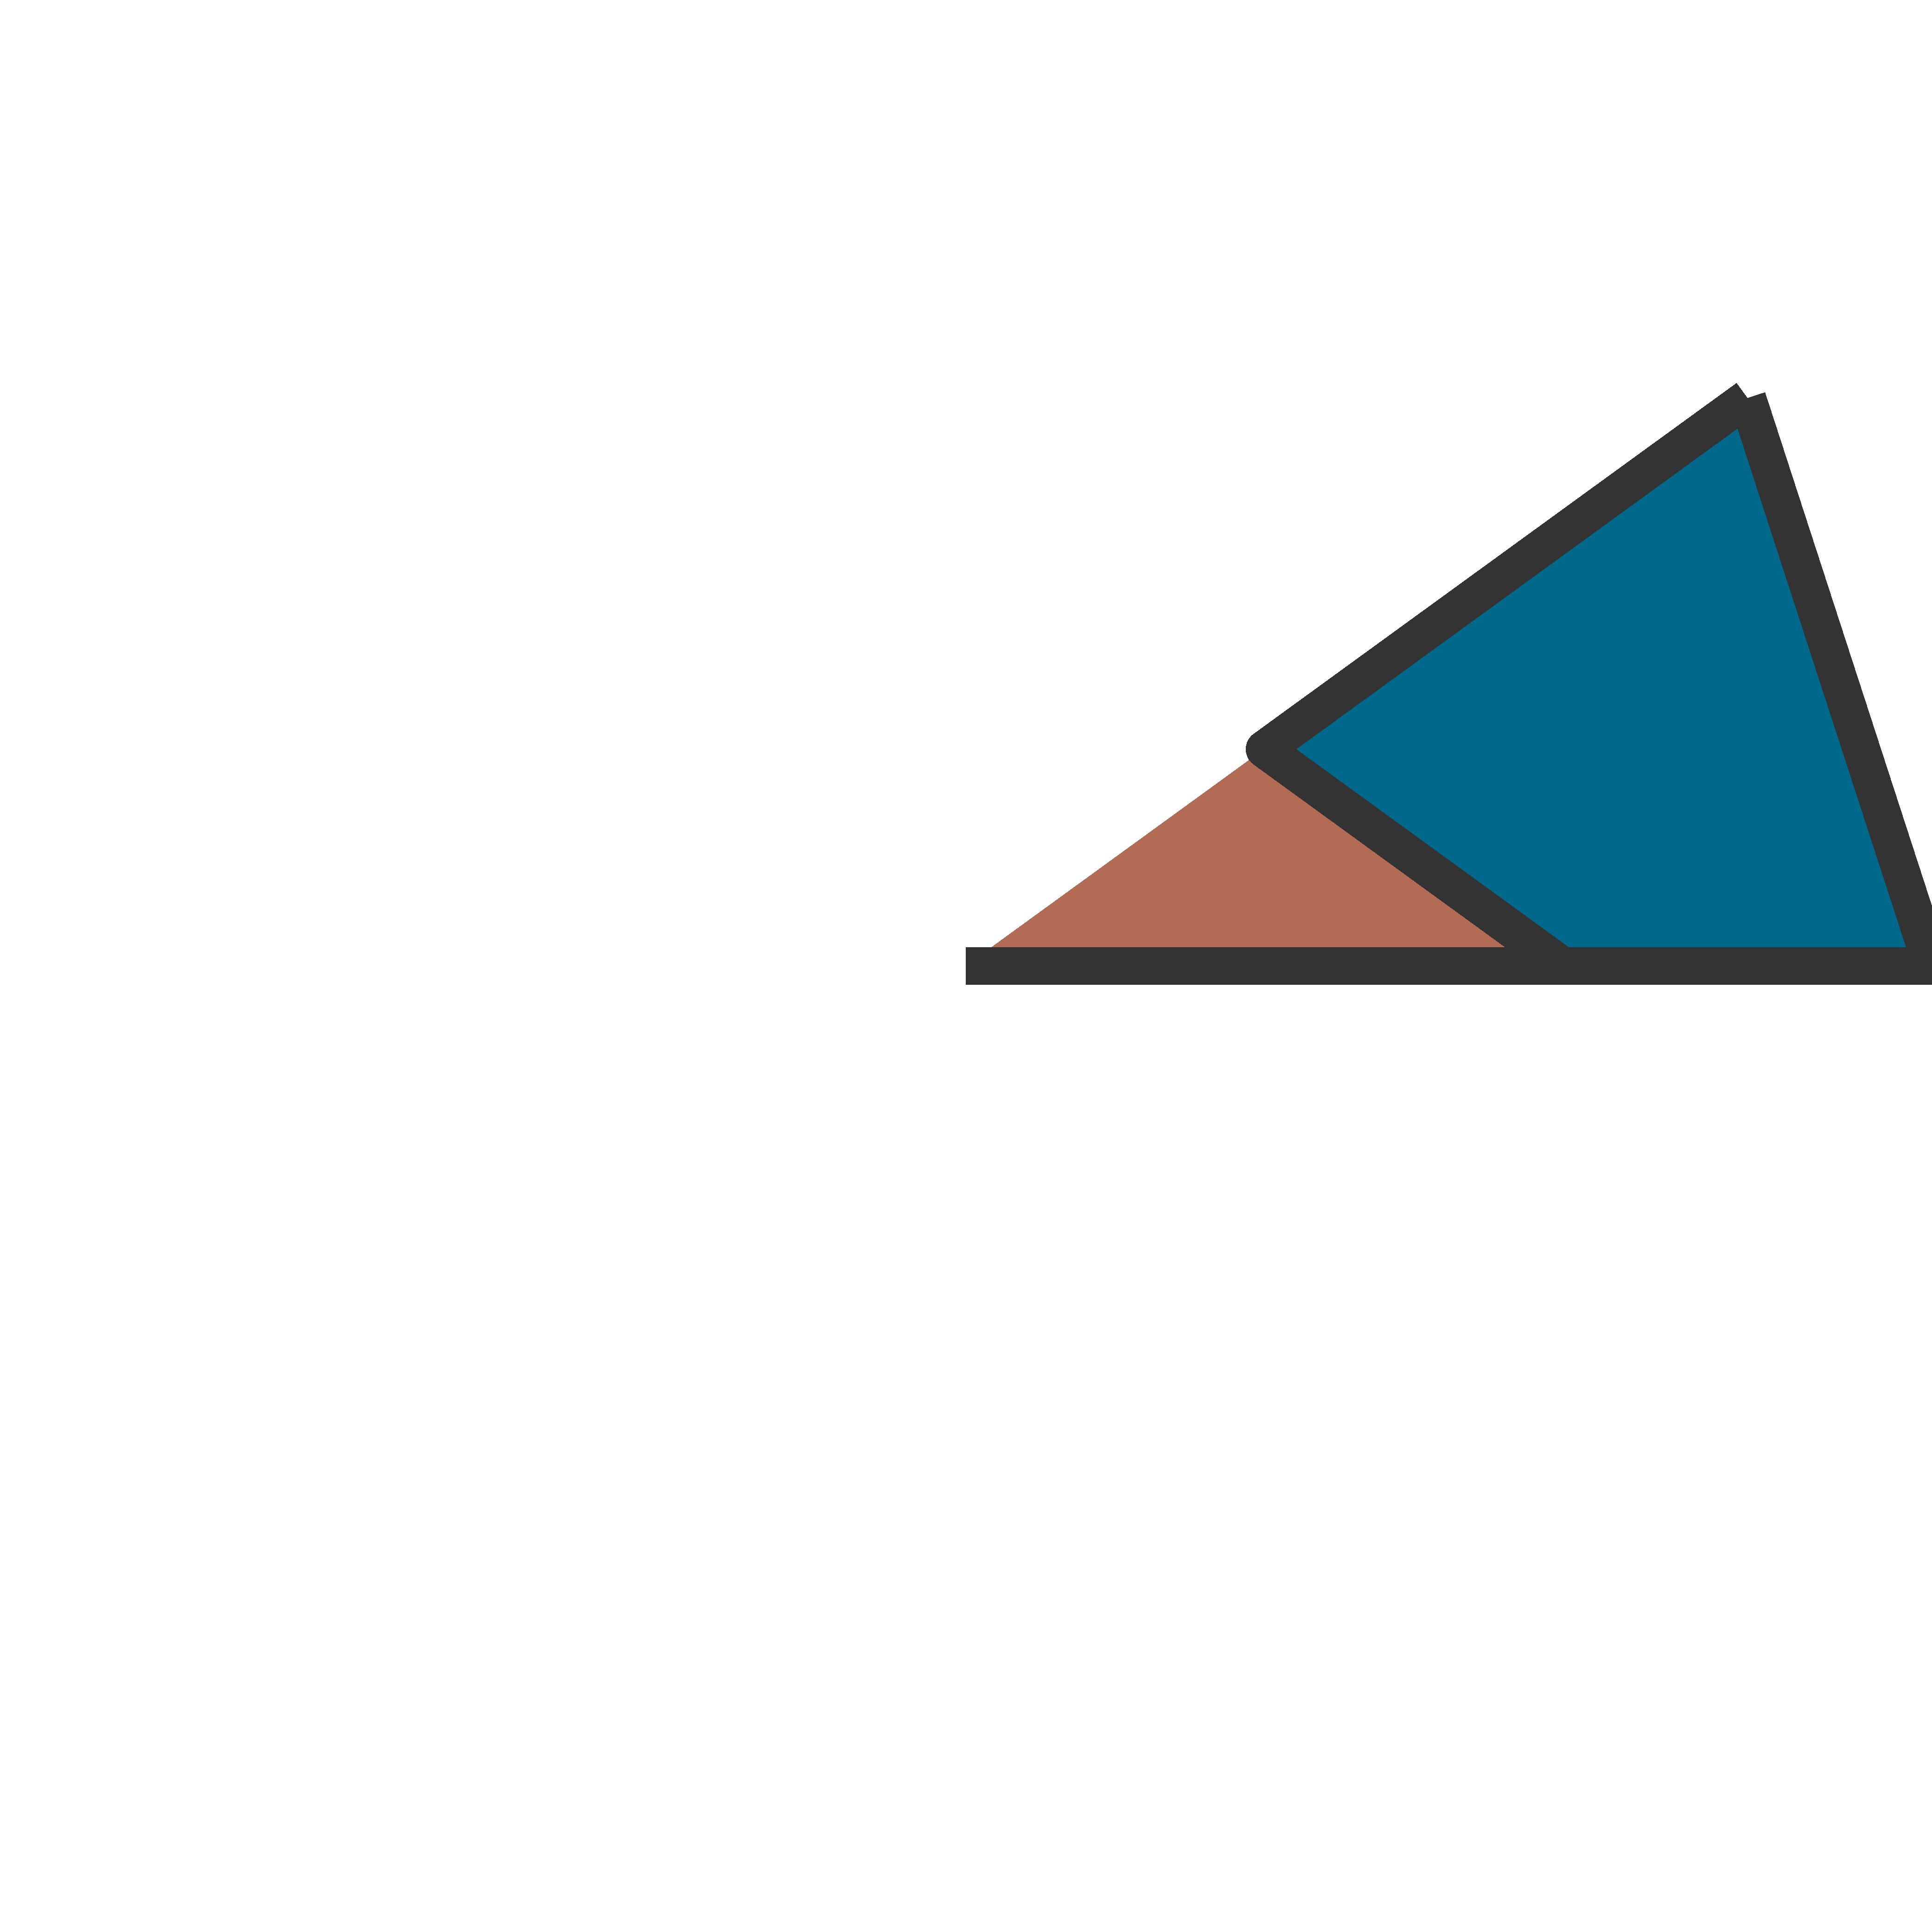
\includegraphics[width=0.8\textwidth]{img/kite_inflated.pdf}
\>
\)
\end{frame}

\end{document}